% FILE: main.tex  Version 2.1
% AUTHOR:
% Universität Duisburg-Essen, Standort Duisburg
% AG Prof. Dr. Günter Törner
% Verena Gondek, Andy Braune, Henning Kerstan
% Fachbereich Mathematik
% Lotharstr. 65., 47057 Duisburg
% entstanden im Rahmen des DFG-Projektes DissOnlineTutor
% in Zusammenarbeit mit der
% Humboldt-Universitaet zu Berlin
% AG Elektronisches Publizieren
% Joanna Rycko
% und der
% DNB - Deutsche Nationalbibliothek

% Dies ist die Hauptdatei Ihrer Dissertation. Mit * gekennzeichnete
% Elemente sind optional und können durch Entfernen/Hinzufügen des
% %-Zeichens gewählt/abgewählt werden. Weitere Informationen
% entnehmen Sie bitte der beiliegenden Broschüre!

% Dokumentenklasse
\RequirePackage[patch]{kvoptions} 
\documentclass{DissOnlineLatex}
% in DissOnlineLatex geometry
% Einstellungen geändert, da
% Optionsübergabe nicht klappt

\usepackage{setspace}
\usepackage[babel,german=guillemets]{csquotes}
\usepackage[citestyle=authoryear,bibstyle=nejm,sorting=nyt,mincitenames=1,maxcitenames=2,maxbibnames=99]{biblatex}
\DefineBibliographyStrings{ngerman}{
  andothers = {{et\,al\adddot}},
}
\usepackage{varioref}
\usepackage{hyperref}
\usepackage{cleveref}
\usepackage{booktabs}
\usepackage{mathtools}
\usepackage{graphicx}
\usepackage{epigraph}
\setlength\epigraphwidth{8cm}
\setlength\epigraphrule{0pt}
\usepackage{etoolbox}
\usepackage{acronym}
%\usepackage[toc]{glossaries}
%\makeglossary
\makeatletter
\patchcmd{\epigraph}{\@epitext{#1}}{\itshape\@epitext{#1}}{}{}
\makeatother
%wegen Sweave
%\usepackage{color}
%\usepackage{framed}
%\usepackage{alltt}
%\IfFileExists{upquote.sty}{\usepackage{upquote}}{}

\bibliography{bibliography}

% Eigene Trennungsregeln* 
% FILE: hyphenations.tex  Version 2.1
% AUTHOR:
% Universit�t Duisburg-Essen, Standort Duisburg
% AG Prof. Dr. G�nter T�rner
% Verena Gondek, Andy Braune, Henning Kerstan
% Fachbereich Mathematik
% Lotharstr. 65., 47057 Duisburg
% entstanden im Rahmen des DFG-Projektes DissOnlineTutor
% in Zusammenarbeit mit der
% Humboldt-Universitaet zu Berlin
% AG Elektronisches Publizieren
% Joanna Rycko
% und der
% DNB - Deutsche Nationalbibliothek

\hyphenation{Bei-spiel} 
                          
%-zusaetzliche Kommandos*
%% FILE: appendixA.tex  Version 2.1
% AUTHOR:
% Universit�t Duisburg-Essen, Standort Duisburg
% AG Prof. Dr. G�nter T�rner
% Verena Gondek, Andy Braune, Henning Kerstan
% Fachbereich Mathematik
% Lotharstr. 65., 47057 Duisburg
% entstanden im Rahmen des DFG-Projektes DissOnlineTutor
% in Zusammenarbeit mit der
% Humboldt-Universitaet zu Berlin
% AG Elektronisches Publizieren
% Joanna Rycko
% und der
% DNB - Deutsche Nationalbibliothek

% Eigene Befehle k�nnen hier definiert werden

% Dokumentenanfang
\begin{document}

%selbst eingefügt zur Vermeidung von Schusterjungen und Hurenkindern
\clubpenalty=1000
\widowpenalty=1000
\displaywidowpenalty=1000

% Seitennummerierung für Titel, Widmung, Danksagung, Zusammenfassung,
% Inhaltsverzeichnis werden in römischen Zahlen gesetzt
\pagenumbering{roman}
\pagestyle{empty} 

% Titelblatt
% FILE: titlepage.tex  Version 3.0
% AUTHOR:
% Universit�t Duisburg-Essen, Standort Duisburg
% AG Prof. Dr. G�nter T�rner
% Verena Gondek, Andy Braune, Henning Kerstan
% Fachbereich Mathematik
% Lotharstr. 65., 47057 Duisburg
% entstanden im Rahmen des DfG-Projektes DissOnlineTutor
% in Zusammenarbeit mit der
% Humboldt-Universitaet zu Berlin
% AG Elektronisches Publizieren
% Joanna Rycko
% und der
% DNB - Deutsche Nationalbibliothek

%----------Generierung der Titelseite------------------------------------------

\makeatletter % Diese Zeile darf nicht gesl�scht werden!

\title{
\large
\vspace{-3.5cm}
\vspace*{2cm}
Medizinische Fakult�t \\ 
der \\
\@Universitaet \\
\vspace{2cm}
Aus der Klinik f�r internistische Onkologie und H�matologie \\
mit integrierter Palliativmedizin \\
der Kliniken Essen-Mitte \\
\vspace{2cm}
\@Titel \\
\@Untertitel \\
\vspace{2cm}}

\author{
\Large
I n a u g u r a l - D i s s e r t a t i o n \\
zur \\
Erlangung des Doktorgrades der Medizin \\
durch die Medizinische Fakult�t \\
der \@Universitaet \\
\vspace{2cm}
}

\date{
\large
Vorgelegt von \\  \@Anrede\ \@Vorname\ \@Nachname\ \\
aus \@Geburtsort \\2016}

\makeatother % Diese Zeile darf nicht gel�scht werden!

\maketitle

% Widmung*
%% FILE: dedication.tex  Version 2.1
% AUTHOR:
% Universit�t Duisburg-Essen, Standort Duisburg
% AG Prof. Dr. G�nter T�rner
% Verena Gondek, Andy Braune, Henning Kerstan
% Fachbereich Mathematik
% Lotharstr. 65., 47057 Duisburg
% entstanden im Rahmen des DFG-Projektes DissOnlineTutor
% in Zusammenarbeit mit der
% Humboldt-Universitaet zu Berlin
% AG Elektronisches Publizieren
% Joanna Rycko
% und der
% DNB - Deutsche Nationalbibliothek

\thispagestyle{empty}
\vspace*{\fill}
\begin{center}
F�r unsere Patienten.
\end{center}
\vspace*{\fill}


% Danksagung*
%% FILE: acknowledgement.tex  Version 2.1
% AUTHOR:
% Universit�t Duisburg-Essen, Standort Duisburg
% AG Prof. Dr. G�nter T�rner
% Verena Gondek, Andy Braune, Henning Kerstan
% Fachbereich Mathematik
% Lotharstr. 65., 47057 Duisburg
% entstanden im Rahmen des DFG-Projektes DissOnlineTutor
% in Zusammenarbeit mit der
% Humboldt-Universitaet zu Berlin
% AG Elektronisches Publizieren
% Joanna Rycko
% und der
% DNB - Deutsche Nationalbibliothek

%Danksagungen

% Zusammenfassung/Abstract
% FILE: abstract.tex  Version 2.1
% AUTHOR:
% Universit�t Duisburg-Essen, Standort Duisburg
% AG Prof. Dr. G�nter T�rner
% Verena Gondek, Andy Braune, Henning Kerstan
% Fachbereich Mathematik
% Lotharstr. 65., 47057 Duisburg
% entstanden im Rahmen des DFG-Projektes DissOnlineTutor
% in Zusammenarbeit mit der
% Humboldt-Universitaet zu Berlin
% AG Elektronisches Publizieren
% Joanna Rycko
% und der
% DNB - Deutsche Nationalbibliothek

%-englische-Zusammenfassung---------------------------------------
\selectlanguage{english}
\begin{abstract}

\subsection*{The Geriatric-Oncologic Conference, a new approach in
de\-cision-making}

\textbf{Background}\\
A comprehensive geriatric assessment (CGA) is recommended before
treating elderly cancer patients. However, it is not proven that
additional information from the CGA will change our treatment
decision.

\textbf{Methods}\\
421 cancer patients, 65 years or older, were judged by their treating
oncologist regarding fitness for chemotherapy. Accompanying a CGA was
performed and each patient was discussed in a multidisciplinary board
(MB) including a geriatrician. The differences between the judgements
of the treating oncologist, the MB, and a classification based solely
on the CGA were examined. Additionally a statistical model of the
decision making process within the MB, based on the findings of the
CGA was established and evaluated.

\textbf{Results}\\
Treating oncologist and MB judged 12\% and 15\% of the patients as
frail, 41\% and 38\% as vulnerable, 46\% and 47\% as fit. 83\% of
congruence was observed. Based on the proposal of Balducci, 55\% of
the patients were classified as frail, 30\% as vulnerable and 15\% as
fit. 34\% of congruence with treating oncologist judgement was
observed. In the 2-stage logistic model the activities of daily living
and the mini mental state examination (MMSE) discriminated between
frail and vulnerable or fit. Tinetti test, age, Charlson comorbidity
index, living alone, MMSE and mini nutritional assessment
discriminated between vulnerable and fit. The statistical models were
able to differentiate with an accuracy of 95\% between frail and
vulnerable or fit and 83\% between vulnerable and fit.

\textbf{Conclusions}\\
To our experience, the judgement of an experienced oncologist is well
comparable with the judgement of a MB. Nevertheless, for some patients
discussion of CGA data in the MB may essentially change treatment
decisions. A logistic regression model of the decision making process
within the MB may replace the elaborate team discussion, if a
conference is not feasible.

\end{abstract}

%-deutsche Zusammenfassung----------------------------------------
\selectlanguage{ngerman}

\section*{Abstract}

\textbf{Hintergrund}\\
Vor der Behandlung geriatrisch-onkologischer Patienten sollte ein
umfassendes geriatrisches Assessment (CGA) durchgef�hrt werden. Es ist
jedoch unklar, inwieweit die erhobenen Zusatzinformationen die
Behandlungsentscheidung beeinflussen.

\textbf{Methoden}\\
421 onkologische Patienten, ab 65 Jahren, wurden durch ihren
behandelnden Onkologen bez�glich der Durchf�hrbarkeit einer
Chemotherapie eingesch�tzt. Begleitend wurde ein Assessment
durchgef�hrt und die Ergebnisse in einer interdisziplin�ren Konferenz
an der auch ein Geriater beteiligt war, besprochen. Die Unterschiede
beider Einsch�tzungsm�glichkeiten und einer Klassifikation, die allein
auf die Ergebnisse des Assessments beruht, wurden
untersucht. Zus�tzlich wurde ein statistisches Modell des
Entscheidungsprozesses der interdisziplin�ren Konferenz erstellt und
analysiert.

\textbf{Ergebnisse}\\
Die behandelnden Onkologen und die interdisziplin�re Konferenz
beurteilten 12\% und 15\% der Patienten als nicht therapief�hig, 41\%
und 38\% als eingeschr�nkt therapief�hig und 46\% und 47\% als
uneingeschr�nkt therapief�hig. In 83\% der F�lle wurde gleich
entschieden. Nach dem Vorschlag von Balducci wurden 55\% der
Patienten als nicht therapief�hig, 30\% als eingeschr�nkt
therapief�hig und 15\% als uneingeschr�nkt therapief�hig
klassifiziert. In 34\% der F�lle herrschte �bereinstimmung mit
der Beurteilung des behandelnden Onkologen. In einer zweistufigen
logistischen Regression unterschieden der Barthel-Index und der
Mini-Mental-Test zwischen nicht therapief�hig und
therapief�hig. Tinetti-Test, Alter, Charlson-Komorbidit�tsindex,
Mini-Mental-Test und Ern�hrungsassessment unterschieden zwischen
eingeschr�nkt und uneingeschr�nkt therapief�hig. Die Modelle
prognostizierten die Konferenzentscheidung in
95\% der F�lle bez�glich nicht therapief�hig und therapief�hig und
83\% der F�llt bez�glich eingeschr�nkt oder uneingeschr�nkt
therapief�hig korrekt.

\textbf{Schlussfolgerung}\\
Nach unserer Erfahrung ist die Beurteilung eines erfahrenen Onkologen
durchaus vergleichbar mit der Beurteilung einer interdisziplin�ren
Konferenz. Allerdings k�nnen f�r einzelne Patienten die in einem
Assessment erhobenen Zusatzinformationen durchaus
entscheidungsrelevant sein. Ein statistisches Modell k�nnte
gegebenenfalls die aufw�ndige Entscheidungsfindung in einer
interdisziplin�re Konferenz ersetzen, wenn diese nicht m�glich ist.

  
% Inhalts-, Abbildungs*-, Tabellen*-Verzeichnis
\tableofcontents

% Kapitel
\onehalfspacing % eigener Befehl aus dem empfohlenen Paket setspace,
                % Deckblätter auch mit anderthalbfachem Zeilenabstand?
                % Dann Befehl an den Anfang stellen

% Definition der Ergebnisse, nur hier berechnete Daten eingeben,
% später im Text dann nur per Variablennamen ansprechen.

% Beschreibung der analysierten Patienten
\newcommand{\ersterPatient}{Januar 2014}
\newcommand{\letzterPatient}{Oktober 2015}
\newcommand{\nPatients}{384} % Gesamtzahl der Patienten
\newcommand{\nMale}{211}
\newcommand{\nFemale}{173}
\newcommand{\percentMale}{55}
\newcommand{\percentFemale}{45}
\newcommand{\alterMedian}{76}
\newcommand{\alterMin}{60}
\newcommand{\alterMax}{94}
\newcommand{\nWeightHeight}{378}
\newcommand{\percentWeightHeight}{98}
\newcommand{\meanHeight}{169}
\newcommand{\sdHeight}{8}
\newcommand{\meanWeight}{74}
\newcommand{\sdWeight}{16}
\newcommand{\meanBmi}{25,8}
\newcommand{\sdBmi}{5,0}
\newcommand{\nUnterAltersDef}{10}
\newcommand{\percentGeriatrischOnkologie}{54}
% zwei Abbildungen: altersverteilung.pdf und altersverteilungAllgemein.pdf

% Barthel-Index
\newcommand{\nBarthel}{378}
\newcommand{\percentBarthel}{98}
\newcommand{\barthelMax}{100}
\newcommand{\percentBarthelMax}{52}
\newcommand{\medianBarthel}{100}

% IADL
\newcommand{\nIadl}{361}
\newcommand{\percentIadl}{94}
\newcommand{\iadlMax}{8}
\newcommand{\percentIadlMax}{37}
\newcommand{\medianIadl}{6}

% Tinetti
\newcommand{\nTinetti}{366}
\newcommand{\percentTinetti}{95}
\newcommand{\tinettiMax}{28}
\newcommand{\tinettiMin}{0}
\newcommand{\percentTinettiMax}{23}
\newcommand{\percentTinettiMin}{1}
\newcommand{\medianTinetti}{24}
\newcommand{\percentTinettiModerateRisk}{19}
\newcommand{\percentTinettiHighRisk}{32}

%TUG
\newcommand{\nTug}{335}
\newcommand{\percentTug}{87}
\newcommand{\tugNotPossible}{39}
\newcommand{\tugMin}{5}
\newcommand{\tugMax}{120}
\newcommand{\medianTug}{10}

% MMST
\newcommand{\nMmst}{347}
\newcommand{\percentMmst}{90}
\newcommand{\mmstMax}{30}
\newcommand{\percentMmstNormal}{78}
\newcommand{\percentMmstLight}{19}
\newcommand{\percentMmstModerate}{2}
\newcommand{\percentMmstSevere}{0}

% DEMTECT
\newcommand{\nDemtect}{130}
\newcommand{\percentDemtect}{80}
\newcommand{\DemtectMax}{18}
\newcommand{\percentDemtectMax}{18}
\newcommand{\percentDemtectNormal}{61}
\newcommand{\percentDemtectLight}{25}
\newcommand{\percentDemtectDemenz}{15}

%GDS
\newcommand{\nGds}{115}
\newcommand{\percentGds}{91}
\newcommand{\gdsMax}{14}
\newcommand{\gdsMin}{0}
\newcommand{\percentGdsNormal}{77}
\newcommand{\percentGdsSuspect}{20}
\newcommand{\percentGdsDepression}{3}

%DIA-S
\newcommand{\nDia}{235}
\newcommand{\percentDia}{91}
\newcommand{\diaMax}{10}
\newcommand{\percentDiaNormal}{52}
\newcommand{\percentDiaSuspect}{11}
\newcommand{\percentDiaDepression}{36}

%Charlson
\newcommand{\nCharlson}{366}
\newcommand{\percentCharlson}{95}
\newcommand{\percentCharlsonZero}{34}
\newcommand{\percentCharlsonThreeOrMore}{23}

%MNA
\newcommand{\nMna}{322}
\newcommand{\percentMna}{84}
\newcommand{\mnaNormal}{34}
\newcommand{\mnaRisk}{50}
\newcommand{\mnaMalnourished}{16}

%Soziale Situation
\newcommand{\nSocialStatus}{347}
\newcommand{\percentSocialStatus}{90}
\newcommand{\percentSocialAlone}{30}

%Persönliche Einschätzung
\newcommand{\nPersonal}{320}
\newcommand{\percentPersonal}{96}
\newcommand{\percentPersonalGogo}{47}
\newcommand{\percentPersonalSlowgo}{41}
\newcommand{\percentPersonalNogo}{12}

%Konferenzeinschätzung
\newcommand{\nKonferenz}{359}
\newcommand{\nKonferenzNa}{25}
\newcommand{\percentKonferenz}{93}
\newcommand{\percentKonferenzGogo}{47}
\newcommand{\percentKonferenzSlowgo}{39}
\newcommand{\percentKonferenzNogo}{14}

%Vergleich Persönlich Konferenz
\newcommand{\nKonferenzPersonal}{305}
\newcommand{\percentAgreementKP}{84}

%Balducci
\newcommand{\nBalducci}{342}
\newcommand{\percentBalducci}{89}
\newcommand{\percentBaludcciGogo}{15}
\newcommand{\percentBalducciSlowgo}{30}
\newcommand{\percentBalducciNogo}{55}

%Vergleich Persönlich Balducci
\newcommand{\nBalducciPersonal}{293}
\newcommand{\percentAgreementBP}{34}

%Vergleich Balducci Konferenz
\newcommand{\nBalducciKonferenz}{331}
\newcommand{\percentAgreementBK}{21}

% Ende Ergebnisdefinition % eigene ergebnisse.tex Datei mit den
                     % numerischen Ergebnissen, benötigt für
                     % chapter03.tex

% Seitennummerierung im Hauptteil

\setcounter{page}{1}
\pagenumbering{arabic}
\pagestyle{myheadings} 

% FILE: main.tex  Version 2.1
% AUTHOR:
% Universit�t Duisburg-Essen, Standort Duisburg
% AG Prof. Dr. G�nter T�rner
% Verena Gondek, Andy Braune, Henning Kerstan
% Fachbereich Mathematik
% Lotharstr. 65., 47057 Duisburg
% entstanden im Rahmen des DFG-Projektes DissOnlineTutor
% in Zusammenarbeit mit der
% Humboldt-Universitaet zu Berlin
% AG Elektronisches Publizieren
% Joanna Rycko
% und der
% DNB - Deutsche Nationalbibliothek

\chapter{Einleitung}

\epigraph{``Begin at the beginning,'' the King said gravely, ``and go
  on till you come to the end: then stop.''}{--- \textup{Lewis
    Carroll, Alice in Wonderland}}

\section{Das t�gliche Dilemma}
\label{sec:geriatrische_onkologie}

An manche meiner Patienten kann ich mich besonders lebhaft
erinnern. Vor drei Jahren lernte ich Frau K. kennen, die gerade
aufgrund ihrer chronisch lymphatischen Leuk�mie von einem Kollegen
eine Immun-Chemotherapie bekam. Zu dieser Zeit war sie bereits 91
Jahre alt. Wegen ihres Umzugs in die N�he ihrer Familie, stellte sie
sich bei mir zur Fortf�hrung der Behandlung vor. Bisher hatte sie die
Therapie sehr schlecht vertragen.

Ist in diesem Alter eine Chemotherapie sinnvoll? Kann eine
Chemotherapie in diesem Alter �berhaupt noch vertragen werden?
Verl�ngert eine Chemotherapie in diesem Alter das �berleben?
Welchen Patienten kann in diesem Alter eine Chemotherapie
zugemutet werden? Ab welchem Alter wird eine Chemotherapie schlechter
vertragen? Ab welchem Alter sind t�dliche Komplikationen der
Chemotherapie zu h�ufig, um hingenommen zu werden? Welche zus�tzlichen
Parameter neben dem Alter helfen bei der Einsch�tzung unserer
Patienten?

In der Onkologie ist die Abw�gung allt�glich, ob ein Patient in
der Lage ist, die empfohlene Chemotherapie zu vertragen. Manchmal ist
diese Einsch�tzung auch abh�ngig von Faktoren wie der Art und
Aggressivit�t der Tumorerkrankung, in manchen Extremsituationen auch
zum Beispiel vom Ern�hrungszustand oder der geistigen
Verfassung. Immer spielt das Alter der Patienten eine
wichtige Rolle.

Eine 91 j�hrige Frau hat heute eine mittlere Lebenserwartung von etwa
4 Jahren \autocite{Walter2014}. Mit einer angepassten
Chemotherapie konnte die CLL bei der beschriebenen Patientin zweimalig
zur�ckgedr�ngt werden und ihr damit noch drei weitere Jahre mit guter
Lebensqualit�t erm�glicht werden, bevor sie mit 94 Jahren an ihrer
Erkrankung verstarb. Mit der ebenfalls denkbaren anf�nglichen
Entscheidung, keine Therapie zu beginnen oder diese zumindest
bei dem ersten Auftreten von auch nur geringen Nebenwirkungen
abzubrechen, w�re dies nicht m�glich gewesen.

Die Geriatrische Onkologie ist ein Teilgebiet der
H�matologie/Onkologie und besch�ftigt sich mit den Besonderheiten
�lterer Menschen mit Krebserkrankungen.

Kein Onkologe w�rde einen einj�hrigen S�ugling chemotherapeutisch
wegen einer malignen Erkrankung behandeln. In dieser speziellen
Lebensphase des Menschen, charakterisiert durch eine besondere
Verletzlichkeit der sozialen, psychischen und physischen Situation der
kleinen Patienten, bedarf es neben onkologischer auch spezieller
p�diatrischer Expertise. In Deutschland ist daf�r ein eigener
Facharzt zust�ndig.

Aufgrund der demografischen Entwicklung unserer Gesellschaft befinden
sich viele Patienten eines klinisch t�tigen Onkologen ebenfalls in
einer speziellen Lebensphase. Auch die sp�te Lebensphase ist
gekennzeichnet durch eine besondere Verletzlichkeit bezogen auf die
soziale, psychische und physische Situation \autocite{Hubbard2010} der
�lteren Patienten. Um dieser speziellen Situation gerecht zu werden,
bedarf es neben h�matologisch/onkologischer Expertise auch spezieller
geriatrischer Erfahrung. Daher wird von allen beteiligten
Fachgesellschaften die Zusammenarbeit von H�matologen/Onkologen und
Geriatern empfohlen \autocite{Wildiers2014, Hurria2015}. Die Umsetzung
dieser Empfehlung stellt jedoch weiterhin die Ausnahme dar.

Klinisches Ziel der Geriatrischen Onkologie ist eine bestm�gliche,
individuell auf die physische und psychische
Belastbarkeit und die aktuelle Lebenssituation der Patienten angepasste
Behandlung. Dies beinhaltet die Auswahl und Steuerung der spezifischen
antitumor�sen Therapie aber auch die interdisziplin�re Betreuung
der Patienten und ihrer Angeh�rigen unter Einbeziehung
verschiedener Berufsgruppen.

Wissenschaftliches Ziel der Geriatrischen Onkologie ist die
Erforschung der biologischen Besonderheiten von Krebserkrankungen
�lterer Menschen und der physiologischen Besonderheiten des �lteren
Organismus in Bezug auf Krebsentstehung, Krebsentwicklung und Reaktion
auf eine antitumor�se Therapie.

In den meisten Studien zu onkologischen Therapien sind im Vergleich
zum klinischen Alltag �ltere Patienten deutlich unterrepr�sentiert
\autocite{Scher2012}. An diesem Zustand hat sich auch im letzten
Jahrzehnt nichts ge�ndert \autocite{Hurria2014_2}. Daher sind weitere
Ziele der Geriatrischen Onkologie, den Anteil �lterer Patienten in
onkologischen Studien deutlich zu erh�hen und damit der klinischen
Realit�t anzun�hern und auch zus�tzliche Studien durchzuf�hren, die
sich mit den Besonderheiten der Behandlung �lterer Patienten
besch�ftigen. Entscheidend ist, zwischen dem chronologischen Alter und dem
physiologischen Alter zu unterscheiden und begleitende geriatrische Syndrome und
anderen Komorbidit�ten zus�tzlich zu ber�cksichtigen. Geriatrische Syndrome
bezeichnen dabei Geriatrie-typische Problemkonstellationen wie zum
Beispiel das Sturzsyndrom, Immobilit�t, chronische Schmerzsyndrome,
Ess- und Trinkst�rungen, Schluckst�rungen, Demenz, Depression. Diese
Probleme sind einer Diagnose mit speziell entwickelten
Assessmentinstrumenten besonders gut zug�nglich.

Ein Assessment ist dabei ein f�r einen bestimmten Bereich entwickeltes
diagnostischen Hilfsmittel, welches standardisiert bestimmte Befunde
erhebt, quantifiziert und aufgrund des Ergebnisses eine Bewertung und
Beruteilung vornimmt, die wie bei jedem anderen diagnostischen Test
ebenfalls einer wissenschaftlichen Evaluation zug�nglich sind.

\section{Kurze Geschichte von Assessments}

In der Geriatrie werden seit langer Zeit spezielle
Assessmentinstrumente genutzt \autocite{Leischker2007}. Bereits 1946,
interessanterweise in der gleichen Zeit, in der erstmals systematisch
toxische und zum damaligen Zeitpunkt oft auch t�dliche Chemotherapien
in der Behandlung von Krebserkrankungen eingesetzt wurden, entwickelte
Marjory Warren in England die moderne Form eines Assessments in der
Medizin \autocite{Matthews1984}. Ziel von Warren war es, mit Hilfe
eines Assessments Patienten aus einem heterogenen Patientengut zu
selektionieren, die von medizinischen Interventionen profitieren
k�nnten. Bis heute ist das der prinzipielle Nutzen der verschiedenen
Assessments: aus einer heterogenen Gruppe von Patienten bez�glich
bestimmter Merkmale homogenere Untergruppen zu definieren und zu
selektionieren, die dann Ausgangspunkt bestimmter Interventionen oder
weiterer Untersuchungen sind.

Die erste mir bekannte Ver�ffentlichung zum Stellenwert eines
Assessments erschien 1973, in der Williams und Kollegen den Nutzen
eines ambulanten geriatrischen Assessments zur Vermeidung einer
Pflegeheimeinweisung zeigten \autocite{Williams1973}. Der Nutzen eines
station�ren geriatrischen Assessments wurde erstmals 1984 nachgewiesen
\autocite{Rubenstein1984}. Dabei wurden Patienten, die systematisch
mit Hilfe eines geriatrischen Assessments in einer spezialisierten
geriatrischen Abteilung behandelt wurden, mit Patienten aus der
Normalversorgung verglichen. Zum Entlassungszeitpunkt waren
Patienten, die im Rahmen der Normalversorgung behandelt wurden, in
h�herem Ausma� auf fremde Hilfe angewiesen und wurden h�ufiger in ein
Pflegeheim eingewiesen.

\section{Begriffserkl�rungen}
\label{sec:begriffe}
Der geriatrische Patient ist durch die Deutsche Gesellschaft f�r
Geriatrie definiert als Patient mit Geriatrie-typischer Multimorbidit�t
und h�herem Lebensalter \autocite{Bruder2009}, wobei explizit eine
kalendarische Altersangabe vermieden wird.

Der �ltere Mensch wird in vielen geria\-trisch"=onkolo\-gischen
Arbeiten ab 65 oder 70 Jahren definiert. Diese feste kalendarische
Definition wurde hier mit der Festlegung auf Patienten ab 65 Jahre
�bernommen.

Umfassendes geriatrisches Assessment, geriatrisches Assessment und
Assessment werden synonym verwendet und beschreiben ein in der Geriatrie
gebr�uchliches Erhebungsverfahren mit einer Kombination verschiedener
Tests. Abgek�rzt wird dies in der Literatur mit dem englischen Akronym
CGA, comprehensive geriatric assessment.

Im folgenden Text wird das Wort signifikant auschlie�lich im
statistischen Sinn gebraucht, mit einem wie in der Medizin �blichen
Signifikanzniveau von 0,05.

\section{Epidemiologie}

Die durchschnittliche Lebenserwartung der Menschen hat im vergangenen
Jahrhundert stetig zugenommen. Da die Inzidenz der meisten b�sartigen
Erkrankungen mit steigendem Alter zunimmt, stieg damit auch die
Inzidenz von Krebserkrankungen an. Hinzu kommt bei �lteren Patienten
au�erdem eine erh�hte Inzidienz an Komorbidit�ten und funktionellen
Defiziten. Im Gegensatz zu j�ngeren Tumorpatienten sind �ltere
Tumorpatienten sowohl tumorbiologisch \autocite{Kumar2011} als auch
bez�glich Komorbidit�ten und funktioneller Probleme eine erheblich
heterogenere Patientengruppe.

Bezogen auf den einzelnen Menschen steigt die Krebsinzidenz in den
letzten Lebensdekaden exponentiell. Mehr als 60\% aller neu
diagnostizierter Krebserkrankungen und sogar mehr als 70\% der
Krebstodesf�lle betreffen Patienten, die 65 Jahre oder �lter sind. Die
altersangeglichene Krebsinzidenz ist bei den gr��er gleich 65 j�hrigen
10 fach h�her, die altersangeglichene Krebsterblichkeit sogar 16 fach
h�her, verglichen mit den unter 65 j�hrigen \autocite{Berger2006,
  Owusu2014, Krebsregister2013}.

Die moderne evidenzbasierte Medizin beruht auf der Durchf�hrung von
randomisierten, kontrollierten Studien. In diesen Studien waren bis
vor kurzem �ltere Patienten von vornherein ausgeschlossen. Dies �ndert
sich zwar in letzter Zeit, so darf allein das Alter in aktuellen
Studien kein Ausschlusskriterium mehr sein, jedoch sind auch heute
noch die �lteren Patienten in gro�en klinischen Studien, inklusive der
Zulassungsstudien der meisten etablierten Chemotherapien und auch
neuer zielgerichteter Substanzen unterrepr�sentiert
\autocite{Scher2012}. Die Ergebnisse dieser Studien sind daher 
nicht auf �ltere Patienten, die nicht Teil des Studienkollektivs
waren, �bertragbar. Im klinischen Alltag muss dies jedoch mangels
Alternativen versucht werden.

\section{Assessments in der Geriatrie}

Das umfassende geriatrische Assessment erfasst multidiziplin�r
verschiedene alters\-assozi\-ierte physiologsiche und psychologische
Faktoren, die Gesundheit und Krankheit �lterer Patienten st�rker
beinflussen k�nnen, als allein das chronologische Alter.

Zus�tzlich ist ein geriatrisches Assessment in der Lage
Funktionseinschr�nkungen zu erkennen, die der routinem��igen �rztlichen
Anamnese und k�rperlichen Untersuchung entgehen \autocite{Alessi1997}.

Daher sind in der Geriatrie verschiedene Assessmentsysteme Teil der
Regelversorgung. Nicht nur zur initialen Erfassung von Problemen,
sondern auch in der Verlaufsbeurteilung der Behandlung, ist diese Art
der multiprofessionellen Erfassung verschiedener Parameter neben der
klassischen �rztlichen Anamnese und k�rperlichen Untersuchung im
Routinebetrieb geriatrischer Abteilungen etabliert.

\section{Assessments in der Onkologie}

\subsection{Notwendigkeit}

Der Beginn der modernen Onkologie liegt in der ersten H�lfte des
zwanzigsten Jahrhunderts mit dem Beginn der systematischen
Verabreichung von zytotoxischen Chemotherapien.  Durch die
Verabreichung von Zellgiften konnten erstmals in der Behandlung von
akuten Leuk�mien und aggressiven Lymphomen, sp�ter dann auch einzelner
solider Tumore wie dem Hodenkarzinom, Patienten mit weit
fortgeschrittener Erkrankung geheilt werden. Wegen der zum Teil
dramatischen Nebenwirkungen dieser Therapien, die oft sogar t�dlich
endeten, besch�ftigten sich die in diesem Bereich t�tigen �rzte von
Beginn an auch mit der Frage, welchen Patienten eine solche Therapie
zugemutet werden kann.

F�r welche Patienten besteht also die M�glichkeit, eine
Besserung der Erkrankung zu erreichen, ohne ihr Leben durch die Therapie
zu stark zu gef�hrden? Die Entscheidung, welche Patienten f�r eine
zytostatische Therapie in Frage kamen, traf der Behandler, im besten
Fall das Behandlungsteam. Oftmals war allein das Alter der Patienten
ein Grund, eine Therapie nicht durchzuf�hren.
Diese Situation hat sich bis heute nicht ge�ndert. Durch moderne
supportive Therapien und Erfahrungen aus kontrollierten Studien sind
die modernen Therapien zwar besser vertr�glich und auch sicherer
geworden, als in den Anf�ngen der Onkologie. Trotzdem handelt es sich
weiterhin um die kontrollierte Verabreichung von Zellgiften, die
potenziell t�dlich verlaufen kann. Jeder Onkologe macht im Verlauf
seines Berufslebens die belastende Erfahrung, Patienten nicht an der
Krebserkrankung sterben zu sehen, sondern an den Folgen der durch ihn
eingeleiteten Therapie.

Zus�tzlich hat sich die wahrgenommene Altersgrenze durch die moderne
Supportivtherapie (Wachstumfaktoren, Antiemetika, Antibiotika, etc.)
und der damit verbundenen Verbesserung der Vertr�glichkeit der
onkologischen Therapien, immer weiter hin zum h�herem Lebensalter
verschoben. Hochdosischemotherapien mit autologen und allogenen
Stammzelltransplantationskonzepten wurden anfangs nur Patienten
verabreicht, die j�nger als 50 Jahre waren. Mit zunehmender Erfahrung
mit diesen Behandlungsformen, wurde das Alter zum Beispiel bei der
autologen Stammzelltransplantation in den letzten Jahren bis auf 75
Jahre nach hinten verschoben.

Durch die Weiterentwicklung der onkologischen Therapie zu einer immer
zielgerichteteren Therapie, die gegen bestimmte Merkmale des Tumors
oder auch gegen das den Tumor umgebene Gewebe gerichtet ist, sind
andere Nebenwirkungen als die der klassischen Zellgifte zu
beobachten. Neue Medikamente, die direkt und zum Teil hoch spezifisch
in den Tumorzellstoffwechsel eingreifen, haben ebenfalls ein v�llig
neues Nebenwirkungsprofil. Auch die aktuell erstmals breit
angewendete, erfolgreiche Beeinflussung des Immunsystems durch
sogenannte Immun-Checkpoint-Inhibitoren bringt durch bisher weitgehend
unbekannte, immunologisch vermittelte Toxizit�ten neue Herausforderungen
mit sich. Mit der besseren Vertr�glichkeit einiger Substanzklassen ist
au�erdem, wie zum Beispiel mit Imatinib oder Ibrutinib, eine
lebenslange, kontinuierliche Verabreichung m�glich. Weitgehend
ungekl�rt sind in diesem Zusammenhang m�gliche Interaktionen bez�glich
Pharmakologie und Pharmakokinetik dieser Substanzen mit den bei �lteren
Patienten in gro�er Zahl eingesetzten Medikamenten, die zur Behandlung
der Begleiterkrankungen n�tig sind.

\subsection{Aktuelle Situation}

Der erste mir bekannte Versuch einer systematischen Erfassung des
Allgemeinzustandes und der Leistungsf�higkeit von Patienten, erfolgte
durch Karnofsky w�hrend der Behandlung von Lungenkarzinompatienten mit
Senfgas, einem chemischem Kampfstoff aus dem ersten Weltkrieg. Initial
nutzte Karnofsky den schon damals so genannten Performance Status
nicht zur Auswahl der Patienten, die eine Therapie erhalten konnten,
sondern mangels moderner Bildgebung zur Messung der Wirksamkkeit der
Chemotherapie �ber eine Besserung des Allgemeinzustandes
\autocite{Karnofsky1948}. Benutzt wird der Karnofsky-Index weiterhin,
um eine �nderung des Allgemeinzustands der Patienten w�hrend einer
Chemotherapie zu dokumentieren, aber auch um Patienten zu
identifizieren, die sich m�glicherweise nicht f�r eine spezifische
Therapie eignen.

Zwei weitere, weitghend deckungsgleiche Skalen sind der ECOG (Eastern
Cooperative Oncology Group) oder WHO (World Health Organisation)
Performance Status, kurz ECOG oder (WHO-)PS. Der Vorteil dieser Skalen liegt
in der Einfachheit und damit m�glichen Einsch�tzung durch den
Behandler nach dem ersten Patientenkontakt. Auch in Therapiestudien
hat die Einsch�tzung des Allgemeinzustandes eines Patienten �ber den
Performance Status gro�e Bedeutung. So ist praktisch in allen
onkologischen Studien ein PS von gr��er 2, bei vielen Studien auch
gr��er 1, Ausschlusskriterium. In der t�glichen Arbeit eines Onkologen
ist diese Art der Einsch�tzung allgegenw�rtig. Patienten mit einem PS
von 4 werden sicherlich nur in sehr besonderen F�llen chemotherapeutisch
behandelt. Vorstellbar w�re zum Beispiel ein junger Patient, der durch
eine akute Leuk�mie in diesem schlechten Allgemeinzustand ist, und bei
dem man damit rechnet, dass eine Reduktion der Tumorlast dies rasch
bessert. Aber auch bei Patienten mit einem PS von drei m�ssen gute
Gr�nde f�r eine spezifische Behandlung vorliegen. Eine intensive
Kombinationstherapie w�rde diesen Patienten wohl auch kein Onkologe
verabreichen.

Dass diese alleinige Einsch�tzung aufgrund des Allgemeinzustands, sei
es durch den Karnofsky-Index oder ECOG/WHO-PS nicht optimal ist, ist
jedem klinisch t�tigen Arzt bewu�t. Aufgrund fehlender Alternativen
ist diese Vorgehen jedoch weiterhin ein breit eingesetzter Standard,
entweder explizit bei der Auswahl von Studienpatienten oder auch
implizit in der pers�nlichen Einsch�tzung des Behandlers vor
Einleitung einer Therapie.

\subsection{Anforderungen an ein geriatrisches Assessment bei
  onkologischen Patienten}
\label{sec:assessment}

Zahlreiche zus�tzliche Umst�nde sind denkbar, die nicht unmittelbar
den Performance Score beeinflussen, jedoch trotzdem Einfluss auf die
Vertr�glichkeit und Toleranz einer spezifischen Therapie haben. So ist
zum Beispiel belegt, dass bei �lteren Krebspatienten der Performance
Score unabh�ngig von den Komorbidit�ten ist \autocite{Extermann1998}.
Zus�tzlich w�rde sich ein fr�he Demenz ebenfalls nicht im Performance
Score wiederfinden, h�tte jedoch gerade bei allein lebenden Patienten
eine erhebliche Bedeutung bei der Planung und Durchf�hrung der
Chemotherapie.

Um zu entscheiden, ob ein individueller �lterer Patient spezifisch
behandelt werden, oder eine rein symptomatische Therapie
stattfinden sollte, stellen sich zwei wesentliche Fragen \autocite{Blanco2015}:

\begin{itemize}
\item Wird der Patient voraussichtlich an der Krebserkrankung sterben,
  oder eher wegen anderer Ursachen oder Komorbidit�ten?
\item Was sind die W�nsche und Erwartungen des Patienten und welche
  Therapie assoziierte Toxizit�t wird toleriert?
\end{itemize}

Ohne ein strukturiertes Assessment laufen die genannten Absch�tzungen
intuitiv im Behandler ab, lediglich auf der Grundlage der beiden
Parameter des biologischen Alters und der klinischen
Einsch�tzung. Dabei besteht Unsicherheit, ob der �ltere Patient die
Therapie tolerieren und davon profitieren kann. Im Endeffekt werden
�ltere Patienten weniger h�ufig chemotherapeutisch behandelt, als es
klinische Leitlinien empfehlen. M�glicherweise tr�gt das zum
schlechteren Behandlungserfolg dieser �lteren Patienten bei
\autocite{Berry2013, Mandelblatt2010, Schrag2001}.

Ziele eines geria\-trisch"=onkolo\-gisches Assessments (Auflistung
nach zunehmender Bedeutung)
\begin{itemize}
\item Absch�tzung der Lebenserwartung
\item Bestimmung der Einschr�nkung der Lebensqualit�t durch die
  Krebserkrankung
\item Absch�tzung der Wahrscheinlichkeit des Auftretens von tumorbedingten
Symptomen
\item Absch�tzung der Vertr�glichkeit/Toxizit�t der m�glichen
  Therapie
\item Absch�tzung der Einschr�nkung der Lebensqualit�t durch die
  m�gliche Therapie
\item Besteht die M�glichkeit, die Therapie zeitgerecht und vollst�ndig durchzuf�hren
\end{itemize}

\section{Geriatrische Onkologie}

Altern ist ein hoch komplexer biologischer Vorgang. Angeborene und
erworbene genetische Ver�nderungen aber auch andere Faktoren wie
Stoffwechselbesonderheiten, immunologische Faktoren oder epigenetische
Ver�nderungen und genetische Polymorphismen spielen eine bedeutende
Rolle. Es resultiert  eine enorme interindividuelle Heterogenit�t der
Krebserkrankung sowie auch der betroffenen Patienten. Damit ist die
ohnehin schon hohe Komplexit�t einer Krebserkrankung noch erheblich
gesteigert.

\subsection{Beurteilung der Behandlungsf�higkeit von Patienten}

Es ist bekannt, dass durch eine Anamnese und k�rperlichen Untersuchung
des Patienten durch den Behandler, wesentliche Einschr�nkungen bei
geriatrischen Patienten verborgen bleiben k�nnen. Daher ist auch die
allein auf die Anamnese und k�rperliche Untersuchung
folgende Einsch�tzung der Therapief�higkeit des Patienten durch den
Behandler wegen m�glicher fehlender wesentlicher Informationen sehr
fehleranf�llig. Ein umfassendes geriatrisches Assessment kann diese
wesentlichen Einschr�nkungen bei geriatrischen Patienten besser
identifizieren \autocite{Alessi1997}.

Ein umfassendes geriatrisches Assessment ist der Versuch, durch
wenige, einfach durchzuf�hrende Tests, eine Datengrundlage f�r
eine Unterteilung des heterogenen Patientenkollektivs zu schaffen.
Balducci und Extermann haben im Jahr 2000 eine Klassifizierung von
Patienten in drei Kategorien vorgeschlagen
\autocite{Balducci2000}.

\begin{enumerate}
\item Patienten, die funktionell unabh�ngig sind und keine
  Komorbidit�t aufweisen und damit Kandidaten f�r jeder Form der
  Standardtherapie sind.
\item Patienten die weder der einen noch der anderen Gruppen
  zuzuordnen sind und damit von einer prim�r reduzierten spezifischen
  Therapie profitieren k�nnten.
\item Patienten, die gebrechlich sind (Abh�ngigkeit in einer oder
  mehreren Aktivit�ten des t�glichen Lebens, drei oder mehr
  Komorbidit�ten, ein oder mehr geriatrisches Syndrom) und damit
  Kandidaten f�r eine rein symptomatische, palliative Therapie sind.
\end{enumerate}

Ber�cksichtigung finden bei diesem Vorschlag drei Werte aus dem
Assessment, der Barthel-Index, der IADL-Score und der
Charlson-Komorbidit�tsindex. �bersetzt in objektivierbare Parameter
aus dem geriatrischen Assessment zeigt dies
Tabelle~\ref{tab:balducci}.

\begin{table}[htbp]
\caption{Vorschlag von Balducci \autocite{Balducci2000}}
\label{tab:balducci}
\centering
\begin{tabular}{llll}
\toprule
Bezeichnung nach Balducci & Barthel & IADL & Charlson \\
\midrule
fit/fit & 100 & 8 & 0 \\
vulnerable/gef�hrdet & 100 & >5 & <3 \\
frail/gebrechlich & <100 oder & <6 oder & >2 \\
\bottomrule
\end{tabular}
\end{table}

Sowohl die Dreiteilung als auch die Bezeichnung der Kategorien ist
willk�rlich, jedoch weit verbreitet. Im angels�chsischen Sprachraum
werden die Kategorien meistens fit oder go go, vulnerable, unfit oder
slow go und frail oder no go genannnt. Ausgehend von dieser
Kategorisierung ist zu bestimmen, inwiefern sie klinisch relevant
ist, also inwiefern sie prognostischen Wert bezogen auf den Verlauf der
Erkrankung und auf die Toxizit�t der Therapie besitzt. Einzelne
Studien zeigen bisher lediglich Zusammenh�nge zwischen wechselnden
einzelnen Parametern des Assessments und der Prognose oder der
Toxizit�t von Chemotherapien.

Die Einteilung durch den Vorschlag von Balducci auf der
Grundlage eines geriatrischen Assessments hat den Vorteil,
dass durch das Assessment zus�tzliche Informationen
gewonnen werden, die dem Behandler bei seiner Einsch�tzung nicht zur
Verf�gung stehen. Der Nachteil jeder Einsch�tzung aufgrund eines
Assessments ist, dass sowohl Art und Stadium der Erkrankung
unber�cksichtigt bleiben, als auch Vertr�glichkeit und Toxizit�t der
m�glichen Therapie. Nachteil speziell der Einteilung nach Balducci
ist, dass nur drei Elemente des multidimensionalen Assessments die
Einteilung beeinflussen. Lediglich die Aktivit�ten des t�glichen
Lebens, also die Pflegebed�rftigkeit gemessen durch den Barthel-Index, die
instrumentellen Aktivit�ten des t�glichen Lebens, also die
Unabh�ngigkeit im Leben gemessen durch den IADL-Score und die Komorbidit�t
gemessen durch den Charlson-Score beeinflussen die Einteilung nach
Balducci. Damit bleiben wesentliche Informationen des Assessments, wie
die geistige Leistungsf�higkeit (MMST) oder die Mobilit�t (TUG und
Tinetti) oder die soziale Situation unber�cksichtigt.

Die Einteilung nach Balducci klassifiziert au�erdem sehr schnell
Patienten als gef�hrdet. Zum Beispiel reicht die Tatsache aus, dass
sie nicht einkaufen oder nicht die W�sche
waschen aus, um Patienten nicht mehr der besten Kategorie zuzuteilen
und somit als gef�hrdet einzustufen.
In einer Ehegemeinschaft mit lange bestehender Aufteilung der
Haushaltspflichten ist dies sicherlich kein gutes Ma�, um eine solche
Unterteilung vorzunehmen. Auch die Einteilung aufgrund der
Komorbidit�t erscheint zumindest fragw�rdig. So sind im
Charlson-Komorbidit�tsscore zwar nur Erkrankungen aufgenommen,
die die Mortalit�t wesentlich beeinflussen \autocite{Charlson1987}.
Jedoch ist anzumerken, dass Erkrankungen
aufgenommen sind, die vor 1987 die Mortalit�t wesentlich beeinflussten.
Dabei ist sicherlich unstrittig, dass mit den heutigen
Behandlungsm�glichkeiten zum Beispiel ein
Diabetes mellitus, der gut medikament�s behandelt ist, kein Grund ist,
einem Patienten die Standardtherapie vorzuenthalten. In der Einteilung
nach Balducci w�re allein dies jedoch der Grund einen Patienten als
gef�hrdet einzustufen. In der Zeit der Evaluation des
Charlson-Komorbidid�tsindexes war sogar ein Magenulcus prognostisch so
bedeutsam, dass es Eingang in den Index gefunden hat. Seit der
Einf�hrung der Protonenpumpeninhibitoren sicherlich kein Grund mehr,
einen Patienten allein aufgrund eines in der Anamnese dokumentierten
Ulcus als gef�hrdet einzustufen.

Es wurde in den letzten Jahren mehrfach festgestellt, dass eine
Klassifikation durch den Behandler mit der Klassifikation
nach dem Vorschlag von Balducci auf der Basis eines geriatrischen
Assessments nur wenig korreliert \autocite{Wedding2007, Tucci2009,
  Tucci2015}.

Die Einteilung durch den Behandler hat jedoch weiterhin den Vorteil,
dass sie die klinische Erfahrung des Behandlers beinhaltet und damit
auch zahlreiche Faktoren, die nur schlecht gemessen werden k�nnen.
Beispiele sind die Art der Tumorerkrankung, eine Einsch�tzung der
aktuellen Situation mit Abw�gung der Probleme, die durch die
Erkrankung hervorgerufen werden, die Einsch�tzung, wie diese mit einer
spezifischen Therapie gebessert werden k�nnen, welche spezifische
Therapie in Frage kommt und wie das Nebenwirkungsprofil dieser
speziellen Therapie ausf�llt.
Der Nachteil ist, dass wesentliche Informationen fehlen k�nnen, weil
der Patient diese nicht mitteilt und Einschr�nkungen vorliegen, die
wie schon ausgef�hrt, der Anamnese und k�rperlichen Untersuchung
entgehen. Diese Tatsache wird durch die pers�nliche Erfahrung vieler
onkologisch t�tiger �rzte best�tigt.
Viele Kollegen sind sich zum Beispiel der Schwierigkeit bewusst, durch
einige wenige Kontakte mit dem Patienten, eine beginnende oder milde
Demenz zu erkennen. Dies kann jedoch w�hrend der Behandlung mit einer
Chemotherapie wesentliche und potentiell t�dliche Probleme
verursachen.

\subsection{Vorhersage von Prognose und Toxizit�t durch geriatrische
  Assessments}
\label{sec:sicherheit}

Die Prognose untersuchte zum Beispiel ein Bericht �ber 348 Patienten,
die 70 Jahre oder �lter waren und aufgrund verschiedener Malignome
eine Chemotherapie bekamen. Das Risiko, innerhalb von sechs Monaten zu
versterben, war mit fortgeschrittener Erkrankung, aber auch mit im
Assessment enthaltenen Tests der Ern�hrungssituation und der
Mobilit�t assoziiert. Nicht assoziiert war das Risko hingegen mit dem in
onkologischen Studien weit verbreiteten ECOG-PS oder anderen im
Assessment enthaltenen Tests zu Selbst�ndigkeit, Kognition 
oder Depression. Interessant ist au�erdem, dass eine durch den
Behandler, der gegen�ber dem Assessment verblindet war, ausgel�ste
prim�re Dosisreduktion der Chemotherapie, also subjektiv empfundene,
eingeschr�nkte Behandlungsf�higkeit, nicht mit dem fr�hen Tod
korrelierte \autocite{Soubeyran2012}. 

In einer Studie an Patienten, 70 Jahre oder �lter, mit aggressiven
Lymphomen, die eine dosismodifizierte CHOP-Therapie erhielten, konnte
das Geriatrische Assessment, speziell ADL und IADL einen fr�hen Tod
vorhersagen \autocite{Soubeyran2014}. Speziell in der Situation der aggressiven
Lymphome ist das f�hrende Dilemma der geriatrischen Onkologie
besonders deutlich sichtbar. Durch aggressivere Therapien auch der
�lteren Patienten konnte die Prognose dieser Patienten in den letzten
Jahren deutlich gesteigert werden \autocite{Kouroukis2002}. Mit der
Aggressivit�t der Therapie steigt jedoch auch die Toxizit�t vor allem
auch bei �lteren Patienten bis hin zu geh�uften therapieassoziierten
Todesf�llen. In einer Serie von Patienten mit
einem aggressivem Lymphom, 65 Jahre oder �lter, konnte gezeigt werden,
dass ein geriatrischen Assessment effektiver in der Vorhersage von
Ansprechen, progressionsfreiem �berleben und Gesamt�berleben war, als die
klinische Einsch�tzung der Behandler \autocite{Feugier2005}.

Ebenfalls bez�glich der Prognose berichteten Maione et al. �ber 566
Patienten, 75 Jahre oder �lter, mit nicht-kleinzelligen
Lungenkarzinom. Das mittlere �berleben war 30 Wochen. Eine
multivariate Analyse f�r prognostische Faktoren ergab einen Einfluss
des IADL-Scores und der Lebenqualit�t, sowie der Anzahl und der Orte
der Metastasierung. Ein allgemeinerer Score als der IADL, der
ADL-Score und auch die Komorbidit�t, gemessen durch den
Charlson-Score, ergab keine zus�tzlichen Informationen bez�glich der
Prognose der Patienten \autocite{Maione2005}.

Eine Assoziation zwischen Parametern des Assessments und der Toxizit�t
einer Chemotherapie zeigte zum Beispiel ein Bericht von 500 Patienten,
die 65 Jahre oder �lter waren und ebenfalls aufgrund verschiedener
Malignome eine Chemotherapie bekamen. Dabei waren Alter, Mobilit�t,
Body Mass Index und Selbst�ndigkeit signifikant mit einer erh�hten
Zahl an schwerer bis t�dlicher Toxizit�t verbunden
\autocite{Hurria2011}.

Eine weitere Studie ebenfalls mit Patienten mit einem
nicht-kleinzelligen Lungenkarzinom, 70 Jahr oder �lter, zeigte eine
Korrelation von Ergebnissen eines geriatrischen Assessments mit
neuropsychiatrischer Toxizit�t und der F�higkeit eine voll dosierte
Chemotherapie zu tolerieren, nicht jedoch mit der Lebensqualit�t
\autocite{Biesma2011}.

Bei Brustkrebspatientinnen, 65 Jahre oder �lter, die eine palliative
Erstlinienchemotherapie erhielten, konnte ein pr�therapeutisch
durchgef�hrtes geriatrisches Assessment Grad 3/4 Toxizit�t der
Chemotherapie voraussagen. Polypharmazie war ebenfalls ein
unabh�ngiger Pr�diktor von Grad 3/4 Toxizit�t durch die
Chemotherapie. Dabei ist unklar, ob dies auch unabh�ngig von der im
Assessment erfassten Komorbidit�t, zum Beispiel durch direkte
Arzneimittelinterationen verursacht wird, oder lediglich, weil
Patientinnen mit h�herer Komorbidit�t auch mehr Medikamente einnahmen
\autocite{Hamaker2014}.

Durch dieses Vorhersagepotential eines Assessments ist aufgrund einer
geriatrisch-onkologsichen Konsultation durchaus eine Beeinflussung des
Therapiekonzeptes denkbar. Eine erste diesbez�gliche Untersuchung
zeigte bei knapp einhundert Patienten bei gut einem Drittel eine
Modifikation des Behandlungsplans \autocite{Girre2008}.

\subsection{Therapeutische Konsequenzen aus Assessments}

Neben der Einsch�tzung der Prognose und der zu erwartenden Toxizit�t
einer onkologischen Therapie k�nnen noch andere Informationen aus dem
Assessment gewonnen werden. Ein geriatrisches Assessment ist
zus�tzlich zur �rztlichen Anamnese und k�rperlichen Untersuchung in
der Lage, Funktionseinschr�nkungen bei �lteren Patienten zu erkennen
\autocite{Alessi1997}. Das Erkennen von Problemen ist jedoch nur der
erste Schritt. Die erkannten Funktionseinschr�nkungen sind h�ufig
medizinisch, physiotherapeutisch oder ergotherapeutisch behandelbar
und damit beinflussbar. Aber auch Probleme die nicht therapeutisch
angehbar sind, wie zum Beispiel die soziale Situation des Patienten,
sind oftmals in Zusammenarbeit mit einem multidisziplin�ren Team
verbesserungsf�hig.

\subsection{Nutzen bei klinischen Studien}

Ein weiteres Ziel der Geriatrischen Onkologie ist, wie in
Abschnitt~\ref{sec:geriatrische_onkologie} bereits erw�hnt, mehr �ltere
Patienten in onkologische Studien einzuschlie�en, um die
�bertragbarkeit der Studienergebnisse in den klinischen Alltag mit
�berwiegend �lteren Patienten zu erm�glichen. Ein Hilfsmittel, um
geeignete �ltere Patienten f�r klinische Studien zu identifizieren,
k�nnte dabei auch ein geriatrischen Assessment sein. Auch innerhalb
einer klinische Studie w�re dies ein wertvolles Instrument, um die
�lteren Patienten genauer zu charackterisieren und ausgehend davon
Toxizit�ten und das �berleben zu untersuchen.

Zus�tzliche Studien sollten au�erdem die Besonderheiten der
Krebserkrankungen �lterer Patienten und die besonderen Reaktionen
�lterer Patienten auf die spezifische Therapie
untersuchen. Dies verspricht nicht nur Erkenntnisse f�r die
t�gliche Arbeit, sondern dar�ber hinaus auch ein zus�tzliches
Verst�ndnis des komplexen Ph�nomens einer Tumorerkrankung.

\subsection{Vorteile f�r den Behandler}

In der H�matologie und Onkologie sind die diagnostizierten
Krankheiten oft lebensbedrohlich. Immer wird eine Krebserkrankung
von Patienten und deren Angeh�rigen als sehr bedrohlich erlebt. In dieser
Situation werden sowohl von Behandlern als auch den Patienten
Ma�nahmen toleriert, die zum Teil mit erheblicher Morbidit�t und
Mortalit�t verbunden sind. Dies gilt ganz allgemein in der Therapie
von Krebskerkrankungen, sei es chirurgisch \autocite{Tegels2014},
strahlentherapeutisch, oder onkologisch durch Chemotherapien.

Jede Sekunde sterben Menschen aus verschiedensten beeinflussbaren
und auch unbeeinflussbaren Ursachen. In der Onkologie ist das Sterben
aufgrund der palliativen Situation der meisten station�ren
Patienten ein gro�er Teil der t�glichen Realit�t. Selbst in dieser
schwierigen Situation kann die moderne Onkologie zusammen mit der
Palliativmedizin viel f�r die Patienten leisten. F�r mich
pers�nlich ist das Sterben meiner Patienten aufgrund ihrer Erkrankung
ein normaler Teil meiner Arbeit, bei dem ich sowohl den Patienten als
auch ihren Angeh�rigen zum Teil trotz des sicheren Ausgangs noch
erheblich helfen kann.

Stirbt ein Patient jedoch nicht an seiner Erkrankung, sondern an der
Therapie, ist die Belastung des gesamten Behandlungsteams deutlich
erkennbar. Auch ist das Leid der Patienten in dieser Situation meiner
Einsch�tzung nach h�her, da palliative, lindernde Therapien wie eine
therapeutische Sedierung m�glicherweise seltener, und Patient und
Angeh�rige belastende intensivmedizinische Therapien m�glicherweise
h�ufiger zum Einsatz kommen.

Wie k�nnen also die Risiken unserer potentiell t�dlichen Therapien
bezogen auf den individuellen Patienten besser eingsch�tzt werden?
In experimentellen, kontrollierten Studien sehen wir die Wirkung, aber
auch die Frequenz und die Schwere der Nebenwirkungen der getesteten
Therapien auf die Studienpopulation. Patient und Behandler m�chten
nicht nur wissen, wie das Medikament in der Studienpopulation gewirkt
hat, sondern auch welche Nebenwirkungen aufgetreten sind. Der Patient,
die Angeh�rigen und der Behandler m�ssen den potentielle Nutzen und
das potentielle Risiko der Therapie, bezogen auf den individuellen
Patienten kennen. Das ist kein spezielles Anliegen der Geriatrischen
Onkologie, sondern der gesamten Medizin.

Die Prognose eines Patienten mit einer Krebserkrankung wird bestimmt
von Stadium und der Art der Krebserkrankung und den Organfunktionen des
Patienten. Dabei spielt weniger das chronologische Alter als das
biologische Alter eine Rolle, also die k�rperliche und psychische
Leistungsf�higkeit sowie eventuell vorhandene Komorbidit�ten.
Routinem��ig teilen �rzte Patienten in jedem Bereich der Medizin in
biologisch �lter und biologisch j�nger ein. Diese pers�nliche und subjektive
Einteilung hat jedoch keine prognostische Relevanz
\autocite{Chow2001}. Manche therapierelevante Defizite im
funktionellen Leistungsverm�gen k�nnen nicht allein durch die Anamnese und
k�rperliche Untersuchung eines einzelnen Arztes entdeckt
werden. Ein interdisziplin�r durchgef�hrtes geriatrisches Assessment
kann unter Zuhilfenahme von standardisierten Testverfahren
im Alter auftretende Funktionsst�rungen h�ufiger erkennen
\autocite{Caillet2014}.

\section{Konzept einer Geriatrischen Onkologie in der Regelversorgung}

Der neue Ansatz, der in dieser Arbeit erstmals verfolgt und
dargestellt wird, besteht darin, beide Verfahren zu kombinieren. Damit
bleiben die Vorteile beider Ans�tze bestehen und die Nachteile
werden behoben. Die Kombination besteht darin, an Hand der Daten, die
in einem Assessment erhoben werden in einer interdisziplin�ren
Konferenz eine Klassifikation vorzunehmen. Damit sind die durch das
Assessment aufgedeckten Probleme zum Zeitpunkt der Beurteilung bekannt.
Aber auch die gerade geschilderten besonderen klinische Situationen
wie zum Beispiel ein sehr gut oder nur sehr schlecht eingestellter
Diabetes k�nnen Ber�cksichtigung finden. Zus�tzlich findet auch die
unsch�tzbare klinische Erfahrung der beteiligten Berufsgruppen
einschlie�lich eines erfahrenen Geriaters und eines speziell
im Bereich der geriatrischen Onkologie t�tigen Onkologen Beachtung.

Die vorliegenden Arbeit beschreibt die Klassifikation von
Patienten ab 65 Jahre durch die geria\-trisch"=onkolo\-gische
Konferenz. Der Beschluss und damit die entsprechende Klassifikation
spiegelt die Beurteilung des Patienten auf der Grundlage der klinisch
zur Verf�gung stehenden und zus�tzlich durch das Assessment erhobenden
Daten wieder.

Denkansto�end f�r diese Arbeit war f�r mich die in meiner Zeit in der
H�matologie h�ufig benutzte Risiko-Einsch�tzung von neu
diagnostizierten AML-Patienten \autocite{Krug2010}. Aufgrund standarm��ig erhobener
Parameter kann dort anhand statistischer Daten einer gro�en Datenbank
von AML-Patienten die Wahrscheinlichkeit einer Remission auf der einen
Seite und das Risiko von Fr�hsterblichkeit auf der anderen Seite,
ermittelt werden. Trotz fehlender prospektiver Validierung ist dies
meiner Meinung nach ein sinnvolles Hilfsmittel f�r die in
Grenzsituationen oft schwierige Entscheidung zwischen einer
potentiell kurativen aber auch potentiell t�dlichen
Induktionschemotherapie oder doch hin zu einer besser vertr�glichen aber
palliativen Chemotherapie.

Genau diese Hilfe k�nnte auch das ebenfalls noch
nicht prospektiv validierte Hilfsmittel eines geriatrischen
Assessments mit anschlie�ender geria\-trisch"=onkolo\-gischer Konferenz
bieten. Neben der Analyse der Unterschiede und Gemeinsamkeiten aller
drei Klassifikationssysteme ist ein praktisches Ziel dieser Arbeit ein
pr�diktives statistisches Modell, welches aus den Assessmentdaten eine
Konferenzentscheidung vorhersagt. Dieses statistische Modell kann
anhand der vorhandenen Daten in seiner Vorhersagegenauigkeit
beschrieben werden und als m�gliches Hilfsmittel bei der Entscheidung
im Internet zur Verf�gung gestellt werden. Bei akzeptabler Fehlerrate
k�nnte ein solches Modell m�glicherweise die Personal- und
Zeit-aufw�ndige geriatrische-onkologische Konferenz ersetzen.

\subsection{Die geriatrisch-onkologische Konferenz}
\label{sec:konferenz}

Die geriatrisch-onkologische Konferenz an den Kliniken Essen-Mitte
setzt sich aus einem Facharzt
f�r Geriatrie, einem Facharzt f�r H�matologie/Onkologie, dem
behandelnden Arzt, und weitere das Assessment durchf�hrende Berufsgruppen
zusammen. Gemeinsam wird auf Grundlage der Informationen die im Rahmen
des Assessments erhoben wurden, eine Einsch�tzung zur
Therapief�higkeit getroffen. Dabei spielen bei der individuellen
Einsch�tzungen auch zus�tzlichen Informationen eine Rolle. Inwieweit
werden die Probleme durch die Tumorerkrankung verursacht? Wie gut
k�nnen diese durch eine spezifische Therapie beeinflusst werden?
Aus diesen �berlegungen und den sich anschlie�enden Diskussionen folgt
der Konferenzbeschluss: Nicht therapief�hig, eingeschr�nkt
therapief�hig oder uneingeschr�nkt therapief�hig.

Die Aussage des Beschlusses muss jedoch relativiert werden. Ehrlicher,
jedoch wenig praktikabel w�re, den Beschluss anders zu formulieren:
"`Wir glauben, der Patient ist uneingeschr�nkt therapief�hig."' Ob die
Einsch�tzung der versammelten Personen in der Konferenz
zutrifft, ist unklar. Es fehlen prospektive, randomisierte
Untersuchungen um eine solche Konferenzentscheidung aber auch die
einzelnen Aussagen der im Assessment enthaltenen Test �ber die Zeit zu
verfolgen und zu �berpr�fen, ob sie richtig war.
Wie beschrieben zeigen Studien, dass ein geriatrisches Assessment die
Toxizit�t einer Therapie voraussagen kann (siehe
Abschnitt~\ref{sec:sicherheit}. Jedoch bleibt bei diesem Ansatz
unklar, ob Patienten, die als nicht therapief�hig eingestuft werden,
wirklich keine denkbare Therapie nutzbringend vertragen h�tten. Ebenso
ist unklar, ob ein Patient, der als eingeschr�nkt
therapief�hig eingesch�tzt wird, nicht doch die maximal denkbare Therapie
vertragen h�tte. All dies bleibt zum jetzigen Zeitpunkt offen und
muss in prospektiven Studien untersucht werden.

Eine pers�nliche Einsch�tzung der Therapief�higkeit durch den
Behandler oder bestenfalls durch das Behandlungsteam findet statt,
seit potentiell toxische Therapien eingesetzt
werden. Da diese Einsch�tzung sehr subjektiv ist und von der pers�nlichen Einstellung
und Erfahrung des Behandlers oder des Teams abh�ngt, wird heute allgemein gefordert,
diese Entscheidung auf der Basis eines umfassenden geriatrischen
Assessments zu treffen. Welche Parameter dabei wie ber�cksichtigt
werden sollten ist offen. Nach einem Vorschlag von Balducci aus dem
Jahr 2000 werden Patienten
anhand des Barthel-Index, der IADL und des Charlson-Komorbidit�tsindex
in eine der drei Kategorien fit, gef�hrdet (vulnerable) und
gebrechlich (frail) eingeteilt \autocite{Balducci2000}. Bei dieser
Einteilung bleibt die Diagnose, die Mobilit�t, die soziale Situation,
die geistige Leistungsf�higkeit und Verfassung sowie die Erfahrung des
Behandlungsteams unber�cksichtigt.

Es bleiben prospektive Daten abzuwarten, ob ein geriatrisches
Assessment allein, zum Beispiel ausgehend vom Vorschlag von Balducci,
oder mit anschlie�ender interdisziplin�rer
geria\-trisch"=onkolo\-gischer Konferenz, diese Absch�tzung besser
vornehmen kann, als der Behandler. Sicher ist jedoch, dass f�r eine
systematische Untersuchung in Studien ein fest definiertes Assessment
besser geeignet ist als die subjektive Einsch�tzung verschiedener
Behandler.

Die vorliegende Arbeit ist der erste mir bekannte Bericht, die
Einsch�tzung der Therapief�higkeit eines Patienten in einer
interdisziplin�ren Konferenz vorzunehmen. In dieser Konferenz sind
die Ergebnisse des Assessments bekannt; zus�tzlich findet jedoch auch
die Erfahrung des Behandlungsteams und der Berufsgruppen, die das
Assessment durchf�hren sowie eines erfahrenen Onkologen und Geriaters
Eingang in die Konferenzentscheidung. Dies hat den offensichtlichen
Vorteil, dass die Entscheidung auf der Grundlage von erhobenen Daten
unter Ber�cksichtigung des klinischen Eindrucks, der Diagnose und der
onkologischen und geriatrischen Expertise getroffen wird. Ob dieser
offensichtliche Vorteil sich auch in einen klinisch messbaren Vorteil
im Sinne besserer Therapievertr�glichkeit oder l�ngeren �berlebens
�bersetzt, sollte in weiteren prospektiven Studien untersucht werden.

Alle bisherigen Untersuchungen zu diesem Thema
vergleichen das Ergebnis des Assessments mit der Entscheidung des
Behandlers und setzten dies in Korrelation mit nachfolgend erhobenen
Daten wie Prognose oder Toxizit�t der Therapie. Dabei wird also allein
anhand der Daten des Assessments, beziehungsweise der Anzahl der
auff�lligen Testergebnisse eine Klassifikation in die drei
Behandlungsgruppen vorgenommen. Das Vorgehen an den Kliniken
Essen-Mitte ist davon
entscheidend abweichend. In der vorliegenden Arbeit wird das
geriatrische Assessment als Zusatzinformation benutzt. Dazu kommen jedoch
innerhalb der geria\-trisch"=onkolo\-gischen Konferenz die so schlecht abbildbare
pers�nliche Einsch�tzung der behandelnden �rzte, der das
Assessment durchf�hrenden Berufsgruppen und des beteiligten Onkologen
und Geriaters hinzu. Im gemeinsamen Gespr�ch wird dann die
Konferenzentscheidung gef�llt, die viele Dinge mit ber�cksichtigen
kann, die allein die Daten des Assessments nicht erfassen. Darunter
f�llt zum Beispiel die Einsch�tzung, wie viele der gemessenen
Einschr�nkungen bereits von der Tumorerkrankung verursacht sind und
auch mit welcher Wahrscheinlichkeit dies durch eine spezifische
Therapie verbesserbar w�re. Aber auch die wahrgenommene pers�nliche
und soziale Situation des Patienten findet Eingang.

In der vorliegenden Arbeit m�chte ich zeigen, dass diese beschriebene
Konferenzentscheidung trotz der vielen dargelegten nicht messbaren
Faktoren in sich konsistent ist und durch ein statistisches Modell
vorhergesagt werden kann. Die Genauigkeit einer solchen Vorhersage
wird analysiert. Zus�tzlich soll gezeigt werden inwieweit die immer
noch am weitesten verbreitete klinische Praxis der pers�nlichen
Einsch�tzung des Behandlers von dieser Konferenzentscheidung abweicht
oder �bereinstimmt. Beides wird dann verglichen mit der in der
Forschung zum geriatrischen Assessment durchgef�hrten Methodik der
Klassifizierung allein aufgrund der Assessmentdaten beziehungsweise
der darin enthaltenden Anzahl der auff�lligen Tests.

\section{Zusammenfassung und Ziele der Arbeit}

Ein umfassendes geriatrisches Assessment ist in der Lage, sowohl
Fr�hsterblichkeit von Tumorpatienten als auch Toxizit�ten von
Behandlungen vorherzusagen und spezifische Behandlungen von erkannten
Defiziten einzuleiten. Inwiefern Prognose und Toxizit�t allerdings von
Entscheidungen, die anhand eines Assessments getroffen werden,
beeinflusst werden k�nnen, also die Behandlung von �lteren 
Tumorpatienten dadurch besser und sicherer gemacht werden kann, ist
unklar. Mindestens drei verschiedenen Ans�tze der Einsch�tzung der
Behandlungsf�higkeit von �lteren Tumorpatienten sind denkbar.

\begin{enumerate}
\item Der Behandler trifft die Therapieentscheidung mit Hilfe der
  zus�tzlichen Informationen aus dem umfassenden geriatrischen
  Assessment.
\item Anhand des umfassenden geriatrischen Assessments werden
  Grenzwerte definiert, ausgehend zum Beispiel von
  \autocite{Balducci2000}, die Patienten in verschiedenen 
  Behandlungsgruppen einteilen, die dann die Therapieentscheidung nach
  sich ziehen.
\item Eine geria\-trisch"=onkolo\-gischen Konferenz bestehend aus dem
  Behandler, einem auch geriatrisch arbeitendem Onkologen, einem Geriater
  und zus�tzlich den Berufsgruppen, die die Tests des Assessments
  durchf�hren, nimmt die Einteilung in die verschiedenen
  Behandlungsgruppen vor, die dann die Therapieentscheidung nach sich
  zieht.
\end{enumerate}

Bis zum Abschluss von prospektiven Studien, die uns den Vergleich der
m�glichen Strategien erlauben, sollte meiner Meinung nach der dritte
Ansatz der derzeitige Goldstandard sein, da dabei die klinischen
Informationen des Behandlers und die zus�tzlichen Informationen, die
ein Assessment bietet, vereint werden und um zus�tzliche geriatrische und onkologische
Expertise erg�nzt werden.

Die vorliegende Arbeit beschreibt die erhobenen Daten und erworbenen
Erfahrungen, die von Januar 2014 bis Dezember 2015 aus der
Zusammenarbeit der Klinik f�r Geriatrie und der Klinik f�r
internistische Onkologie der Kliniken Essen-Mitte gesammelt wurden.
Schwerpunkt ist die Beschreibung eines Kollektivs von �ber 400
Patienten, die 65 Jahre oder �lter waren und bei denen in diesem
Zeitraum ein umfassendes geriatrisches Assessment durchgef�hrt
wurde. Anschlie�end wurde in einer interdisziplin�ren,
geria\-trisch"=onkolo\-gischen Konferenz eine Einsch�tzung bez�glich
der Therapief�higkeit der Patienten abgegeben.

Damit ist dies die erste mir bekannte Beschreibung einer
geria\-trisch"=onkolo\-gischen Zusammenarbeit, die nicht nur ein
Assessment beinhaltet, sondern die interdisziplin�re Konferenz und
damit die individuelle Besprechung der Patienten, unter Einbeziehung
der Assessmentdaten, in den Mittelpunkt der Zusammenarbeit stellt.

Im einzelnen werden in der Arbeit

\begin{enumerate}
\item die Daten eines umfassenden geriatrischen Assessments von �ber
  400 Patienten vorgestellt, die an dieser Klinik 2014 und 2015
  routinem��ig bei allen station�ren Patienten, die 65 Jahre oder
  �lter waren, vor Einleitung einer spezifischen Therapie erhoben
  wurden.
\item wird analysiert, wie die Entscheidung, die anhand der erhobenen
  Daten in einer geria\-trisch"=onkolo\-gischen Konferenz getroffen
  wurde, mit der pers�nlichen Einsch�tzung des behandelnden Arztes und
  der Klassifizierung durch das Assessment korreliert.
\item wird gepr�ft, inwiefern ein statistisches Modell in der Lage ist,
  anhand der Assessmentdaten die Klassifizierung, die innerhalb einer
  aufw�ndigen geria\-trisch"=onkolo\-gischen Konferenz getroffen wird,
  zu modellieren.
\end{enumerate}

% FILE: main.tex  Version 2.1
% AUTHOR:
% Universit�t Duisburg-Essen, Standort Duisburg
% AG Prof. Dr. G�nter T�rner
% Verena Gondek, Andy Braune, Henning Kerstan
% Fachbereich Mathematik
% Lotharstr. 65., 47057 Duisburg
% entstanden im Rahmen des DFG-Projektes DissOnlineTutor
% in Zusammenarbeit mit der
% Humboldt-Universitaet zu Berlin
% AG Elektronisches Publizieren
% Joanna Rycko
% und der
% DNB - Deutsche Nationalbibliothek

\chapter{Methoden}

\section{Die geriatrisch-onkologische Konferenz}

Die geriatrisch-onkologische Konferenz setzt sich aus einem Facharzt
f�r Geriatrie, einem Facharzt f�r H�matologie/Onkologie, dem
behandelnden Arzt, und weitere das Assessment durchf�hrende Berufsgruppen
zusammen. Gemeinsam wird auf Grundlage der Informationen die im Rahmen
des Assessments erhoben wurden aber auch der individuellen
Einsch�tzungen und zus�tzlichen Informationen, wie zum Beispiel
inwieweit ein Teil der Probleme durch die Tumorerkrankung verursacht
ist, oder diese durch eine spezifische Therapie wie gut zu
beeinflussen sind, eine Einsch�tzung zur Therapief�higkeit getroffen. Daraus folgt der
Konferenzbeschluss: Nicht therapief�hig, eingeschr�nkt therapief�hig
oder uneingeschr�nkt therapief�hig steht letztendlich als
Konferenzentscheidung unter dem Protokoll.

Ehrlicher w�re, dort st�nde
z.B.: Wir glauben der Patient ist uneingeschr�nkt therapief�hig. Denn
ob die Einsch�tzung der versammelten Personen in der Konferenz
zutrifft, ist unklar. Es fehlen prospektive, randomisierte
Untersuchungen um eine solche Konferenzentscheidung �ber die Zeit zu
verfolgen und zu �berpr�fen, ob sie richtig war.
Erste Studien zeigen, dass ein geriatrisches Assessment die Toxizit�t
einer Therapie voraussagen kann. Jedoch bleibt bei diesem Ansatz
unklar, ob Patienten, die als nicht therapief�hig eingestuft werden,
wirklich keine denkbare Therapie nutzbringend vertragen h�tten. Ebenso
ist unklar, ob ein Patient, der als eingeschr�nkt
therapief�hig eingesch�tzt wird, nicht doch die maximal denkbare Therapie
vertragen h�tte. All dies bleibt zum jetzigen Zeitpunkt offen und
sollte Gegenstand von prospektiven Studien sein.

Eine pers�nliche Einsch�tzung der Therapief�higkeit durch den
Behandler oder bestenfalls durch das Behandlungsteam findet statt,
seit potentiell toxische Therapien eingesetzt
werden. Da diese Einsch�tzung sehr subjektiv ist und von der pers�nlichen Einstellung
und Erfahrung des Behandlers oder des Teams abh�ngt, wird heute allgemein gefordert,
diese Entscheidung auf der Basis eines umfassenden geriatrischen
Assessments zu treffen. Welche Parameter dabei wie ber�cksichtigt
werden sollten ist offen. Nach einem Vorschlag von Balducci aus dem
Jahr 2000 werden Patienten
anhand des Barthel-Index, der IADL und des Charlson-Komorbidit�tsindex
in eine der drei Kategorien fit, gef�hrdet (vulnerable) und
gebrechlich (frail) eingeteilt \autocite{Balducci2000}. Bei dieser Einteilung bleibt die
Diagnose, die Mobilit�t, die soziale Situation, die geistige
Leistungsf�higkeit und Verfassung sowie die Erfahrung des
Behandlungsteams unber�cksichtigt.

Die vorliegende Arbeit ist der erste mir bekannte Bericht, die
Einsch�tzung der Therapief�higkeit eines Patienten unter Hinzunahme
eines umfassenden geriatrischen Assessments, jedoch unter Einbeziehung
des Behandlungsteams und zus�tzlich weiterer, das Assessment
durchf�hrender Berufsgruppen, eines Onkologen und Geriaters
durchzuf�hren. Dies hat den offensichtlichen Vorteil, dass die
Entscheidung auf der Grundlage von erhobenen Daten unter
Ber�cksichtigung des klinischen Eindrucks, der Diagnose und der
onkologischn und geriatrischen Expertise getroffen wird. Ob dieser
offensichtliche Vorteil sich auch in einen klinisch messbaren Vorteil
im Sinne besserer Therapievertr�glichkeit oder l�ngeren �berlebens
�bersetzt, sollten in weiteren prospektiven Studien untersucht werden.

Alle bisherigen Untersuchungen zu diesem Thema
vergleichen das Ergebnis des Assessments mit der Entscheidung des
Behandlers und setzten dies in Korrelation mit nachfolgend erhobenen
Daten wie Prognose oder Toxizit�t der Therapie. Dabei wird also allein
anhand der Daten des Assessments, beziehungsweise der Anzahl der
auff�lligen Testergebnisse eine Klassifikation in die drei
Behandlungsgruppen vorgenommen. Das Vorgehen an den Kliniken
Essen-Mitte ist davon
entscheidend abweichend. In der vorliegenden Arbeit wird das
geriatrische Assessment als Zusatzinformation benutzt. Dazu kommen jedoch
innerhalb der geria\-trisch"=onkolo\-gischen Konferenz die so schlecht abbildbare
pers�nliche Einsch�tzung der behandelnden �rzte, der das
Assessment durchf�hrenden Berufsgruppen und des beteiligten Onkologen
und Geriaters hinzu. Im gemeinsamen Gespr�ch wird dann die
Konferenzentscheidung gef�llt, die viele Dinge mit ber�cksichtigen
kann, die allein die Daten des Assessments nicht erfassen. Darunter
f�llt zum Beispiel die Einsch�tzung, wie viele der gemessenen
Einschr�nkungen bereits von der Tumorerkrankung verursacht sind und
auch mit welcher Wahrscheinlichkeit dies durch eine spezifische
Therapie verbesserbar w�re. Aber auch die wahrgenommene pers�nliche
und soziale Situation des Patienten findet Eingang.

In der vorliegenden Arbeit m�chte ich zeigen, dass diese beschriebene
Konferenzentscheidung trotz der vielen dargelegten nicht messbaren
Faktoren in sich konsistent ist und durch ein statistisches Modell mit
Hilfe von maschinellem Lernen (logistische Regression, KNN, neuronale
Netze) vorhergesagt werden kann, bzw. mit welcher Genauigkeit eine
solchen Vorhersage getroffen werden kann. Zus�tzlich soll gezeigt
werden inwieweit die immer noch am weitesten verbreitete klinische
Praxis der pers�nlichen Einsch�tzung des Behandlers von dieser
Konferenzentscheidung abweicht oder �bereinstimmt. Beides wird dann
verglichen mit der in der Forschung zum geriatrischen Assessment
durchgef�hrten Methodik der Klassifizierung allein aufgrund der
Assessmentdaten beziehungsweise der darin enthaltenden Anzahl der
auff�lligen Tests.

\section{Elemente des umfassenden geriatrischen Assessments}

Um die oben aufgef�hrten Anforderungen, die an ein geriatrisches
Assessment beim Krebspatienten gestellt werden, zu erreichen wurden
verschiedene einzelne Tests vorgeschlagen. Insgesamt ist mit
zunehmender Erfahrung und prospektiver Evaluation der Tests an
Tumorpatienten die genaue Zusammensetzung der Tests in kontinuierlicher
Entwicklung. In den Kliniken Essen-Mitte hat sich ausgehend von den
aktuellen internationalen
Empfehlungen ein Standard etabliert \autocite{Hurria2014}.

\begin{itemize}
\item Funktioneller Status
  \begin{itemize}
  \item Aktivit�ten des t�glichen Lebens, Barthel Index, ADL
  \item Instrumentelle Aktivit�ten des t�glichen Lebens, IADL
  \item Mobilit�t, Timed up an go Test, TUG
  \item Sturzrisiko, Tinetti-Test
  \end{itemize}
\item Kognitive Funktion
  \begin{itemize}
  \item Mini Mental Status Test, MMST
  \item Demenz-Detektion, DemTect
  \end{itemize}
\item Komorbidit�t
  \begin{itemize}
  \item Charslon-Score
  \item Evaluation geriatrischer Syndrome (z.B. Demenz, Depression,
    Osteoporose, Sturzneigung, Fatique, Urininkontinenz)
  \end{itemize}
\item Polypharmazie
  \begin{itemize}
  \item Anzahl der Medikamente (Definition Polyphamarzie > 4 Medikamente)
  \item Potentiell unangemessene Medikatmente (potentially
    inappropriate medications, PIM)
  \end{itemize}
\item Psychologischer Status
  \begin{itemize}
  \item Geriatrische Depressions Skala, GDS
  \item Depression im Alter-Skala, DIA
  \end{itemize}
\item Soziale Unterst�tzung
  \begin{itemize}
  \item Fragebogen
  \end{itemize}
\item Ern�hrungsstatus
  \begin{itemize}
  \item Mini Nutritional Assessment, MNA, inklusive Gr��e, Gewicht, BMI
  \end{itemize}
\end{itemize}

Das geriatrisches Assessment, das in dieser Arbeit benutzt wurde,
entwickelte sich in unserer Klinik kontinuierlich gem�� den in der
t�glichen Anwendung gewonnenen
Erfahrungen. Begonnen wurde mit den in Tabelle ? gezeigten
Tests.
 
Aufgrund h�ufigen klinischen Verdachts einer Demenz und grenzwertiger
MMST Ergebnisse f�hrten wir auf Veranlassung in der Konferenz noch
zus�tzlich den Dem\-Tect wegen
der h�heren Sensitivit�t bez�glich der Detektion einer Demenz
durch. Dies f�hrte h�ufig zu Verz�gerungen, oder fehlender Werte, da
der Patient bereits entlassen war. Dadurch entschlossen wir uns zu
einer gleichzeitigen Durchf�hrung von MMST und Dem\-Tect.

Tabelle zeitlicher Verlauf der Tests 

\subsection{Komorbidit�t}

Komorbidit�ten erfasst durch den Charlson-Score korellieren nur gering
mit dem funktionellen Status \autocite{Balducci2000}. Daher liefert der
Charlson-Score eine vom funktionellen Status unabh�nige, zus�tzliche
haupts�chlich prognostische Information. Die Lebenserwartung von
�lteren onkologischen Patienten wird wesentlich von den Komorbidit�ten
mitbestimmt \autocite{Extermann2000}. Die Komorbidit�t hat auf die Vertr�glichkeit
einer Chemotherapie einen �hnlich starken Einfluss wie der
funktionelle Status \autocite{Frasci2000}. Der Charlson-Komorbidit�tsindex ist
f�r die Erfassung der Komorbidit�t bei �lteren Tumorpatienten
validiert \autocite{Charlson1987, Charlson1987_1}.

MEMO: Noch Erkl�rung, wie der
Charlson Score zustande kommt. Erh�hung der Mortalit�t etc.

\subsection{Aktivit�ten des t�glichen Lebens, ADL, Barthel-Index}

1965 wurde von der Physiotherapeutin Barthel und der �rztin Mahoney
ein Instrument zur  Verlaufsbeurteilung des funktionellen Status von
Patienten mit neuromuskul�ren und muskulosskelettalen Erkrankungen
entwickelt, welches bis heute als Barthel-Index verwendet wird. Der
Barthel-Index ist einfach zu erheben und gibt die F�higkeit zur
Selbstversorgung wieder. F�r die Aktivit�ten Essen, Aufsetzen und
Umsetzen, sich waschen, Toilletenbenutzung, Baden und Duschen,
Aufstehen und Gehen, Treppensteigen, An- und Auskleiden,
Stuhlkontinenz, Harnkontinenz wird erfasst, ob sie selbst�ndig, mit
Hilfe oder nicht ausgef�hrt werden k�nnen. Die einzelnen drei- oder
viergeteilten Beurteilungn addieren sich zu einer diskreten Verh�ltniskala von
0 bis 100 Punkten. 0 Punkte zeigt dabei v�llige Pflegebed�rftigkeit,
100 Punkte v�llige Selbst�ndikeit an. Ab etwa 80 Punkten ist eine
weitergehende Erfassung mit den Instrumentellen Aktivit�ten des
t�glichen Lebens sinnvoll.

-> Abbildung

\subsection{Instrumentelle Aktivit�ten des t�glichen Lebens, IADL}

Dieser Score gibt die F�higkeit zur selbst�ndigen
Lebensf�hrung wieder. Beurteilt werden die F�higkeit zu telefonieren,
einzukaufen, zu kochen, den Haushalt zu f�hren, die W�sche zu waschen,
zur Benutzung von Transportmitteln, zur Medikamenteneinnahme, sowie zum
Umgang mit Geld. Maximal k�nnen 8 Punkte erreicht werden. Wegen der
fr�her �blichen Aufteilung der Haushaltsf�hrung erreichen M�nner auch
ohne Einschr�nkungen h�ufig nicht die volle Punktzahl. Im hohen
Punktzahlbereich des Barthel-Index und im niedrigen Bereich der IADL
beobachtet man eine �berlappung beider Skalen.

-> Abbildung

\subsection{Kognition}
\label{sec:kognition}

Ein kognitives Assessment bei onkologischen Patienten ist wichtig, um
subklinische kognitive Defizite fr�hzeitig zu erfassen. Damit kann
entscheidend die m�gliche Compliance aber auch Entscheidungsf�higkeit
zumeist komplexischer onkologischer Fragestellungen beurteilt
werden. Jeder klinisch t�tige Kollege kennt aus eigener Erfahrung die
Situation, dass im routinem��igen Umgang mit Patienten eine leichte
Demenz nicht erkannt wird, oder auf Grund verschiedener Umst�nde
�berbewertet wird.

Das international am h�ufigsten verwendete Screeninginstrument f�r
kognitive Defizite ist der Mini-Mental-Status-Test nach Folstein
\autocite{Folstein1975}. Mit maximal 30 zu vergebenen Punkten werden
zeitliche und �rtlicher Orientierung, das Kurzzeitged�chtnis, Lesen,
Schreiben und konstruktive F�higkeiten (Zeichnen) abgefragt. Unter 26
Punkte besteht Demenzverdacht. Allerdings ist der MMST zur Erkennung
leichter Demenzen nicht gut geeignet. 

Besonders gut zur Erkennung leichter kognitiver Einbu�en eignet sich
der Dem\-Tect-Test \autocite{Kalbe2004}. Ausgewertet wird f�r unter 60
j�hrige und �ber 60 j�hrige getrennt. Maximal sind 18 Punkte
erreichbar, bei weniger als 8
Punkten besteht der Verdacht auf das Vorliegen einer Demenz.

Der Dem\-Tect-Test, Demenz-Detektions-Test, wird an den Kliniken
Essen-Mitte seit Februar 2015 zus�tzlich regelhaft durchgef�hrt, um die
zus�tzliche Sensitivit�t in der Erkennung einer klinisch sehr
relevanten, fr�hen Demenz hat, zu nutzen.

\subsection{Depression}
\label{sec:depression}

Jeder Mensch geht anders mit einer belastenden Lebenssituation um. Die
Grenze zwischen normaler Traurigkeit aufgrund schlechter Nachrichten
und einer interventionsbed�rftigen Depression ist flie�end. Oft werden
jedoch auch vorbestehende Depressionen, eine h�ufige Diagnose bei
geriatrischen und onkologischen Patienten vom Behandler nicht
erkannt. Ein Screening auf das Vorliegen einer Depression kann anhand
der Geriatric Depression Scale erfolgen \autocite{Yesavage1982}. Gestellt werden 15
Fragen, die mit Ja oder Nein beantwortet werden. Ein Punktwert von
mehr als 5 spricht f�r das Vorliegen einer Depression.

Die Erfahrung bei der Anwendung des GDS der Ergotherapeutin zeigte, das die in
diesem Test gestellten Fragen, von Patienten mit neu diagnostizierter
Krebserkrankung zum gro�en Teil mit gro�em Befremden aufgenommen
werden. Problematisch waren zum Beispiel Fragen wie: 'Finden Sie es
sch�n, jetzt zu leben?' oder 'Kommen Sie sich in Ihrem jetzigen
Zustand ziemlich wertlos vor?' Nach Absprache mit dem kooperierenden
Geriater wurde ab September 2014 der GDS gegen den DIA-S getauscht.
Verweis ANHANG Die Aussagen dieses Tests wurden durch die Patienten
deutlich positiver aufgenommen.

\subsection{Mobilit�t}

Eine eingeschr�nkte Mobilit�t beeintr�chtigt die Lebensqualit�t
erheblich. Ein erh�htes Sturzrisiko korelliert au�erdem mit erh�hter
Mortalit�t, weiterem Verlust von Mobilit�t und funktioneller
Selbst�ndigkeit und h�ufigen Krankenhausaufenthalten. Ein Drittel
aller Menschen im Alter �ber 65 Jahre und die H�lfte aller �ber
90-J�hrigen st�rzt pro Jahr mindestens einmal \autocite{Trilling1995}.
Der Timed up and go-Test \autocite{Podsiadlo1991} ist schnell und einfach
durchzuf�hren. Aus dem Sitzen auf einem Stuhl wird der Patient
angewiesen aufzustehen, drei Meter zu gehen und sich wieder
hinzusetzen. Hilfsmittel d�rfen dabei verwendet werden. Die ben�tigte
Zeit wird gemessen. Unter zehn Sekunden ist von einer
uneingeschr�nkten Mobilit�t im Alltag ausgegangen werden. Eine Zeit
von 10 bis 19 Sekunden zeigt eine eingeschr�nkte Mobilit�t an, die
jedoch noch zu keiner Einschr�nkung im Alltag f�hrt. Ab einer Zeit von
20 Sekunden muss von einer Beeintr�chtigung in den Aktivit�ten des
t�glichen Lebens ausgegangen werden.
Ein fehlender Wert im Timed-up-and-go-Test (TUG) kann in den
vorliegenden Daten zwei verschiedene Dinge bedeuten. Entweder wurde
der Test nicht durchgef�hrt, oder aber er war nicht m�glich, zum
Beispiel aufgrund Bettl�gerigkeit. Um diese wichtige Information nicht
zu verlieren wurde eine zus�tzliche Variable eingef�hrt, die anzeigt,
ob die Durchf�hrung des Tests m�glich war.

Beim zweiteiligen Tinetti-Test
\autocite{Tinetti1986} werden im ersten Teil Standsicherheit und Balance �berpr�ft
und im zweiten Teil das Gangbild analysiert. Maximal sind 28 Punkte
erreichbar, bei weniger als 20 Punkten ist das Sturzrisiko erh�ht.

\subsection{Ern�hrung}

Der Ern�hrungszustand eines Patienten bestimmt ma�geblich den
Allgemeinzustand mit. Mangelern�hrung vermindert die allgemeine
Leistungsf�higkeit und speziell auch die Vertr�glichkeit einer
Chemotherapie. Zus�tzlich k�nnen Probleme wie �belkeit oder Schw�che,
die durch die Tumorerkrankung oder die Chemotherapie ausgel�st werden,
den Ern�hrungszustand weiter verschlechtern. Der h�ufigste Grund einer
Mangelern�hrung bei geriatrischen Patienten ist eine Depression. Aber
auch Ursachen wie ein schlechter Zahnstatus oder ungen�gende
Kaufunktion sind h�ufig. In 43 \% wird jedoch keine spezifische
Ursache gefunden \autocite{Wilson1998}. Der Body Mass Index (BMI) ist ein besseres
Ma�, der das Gewicht im Verh�ltnis zur K�rpergr��e ber�cksichtigt.

\begin{equation}
\label{eq:bmi}
\text{BMI} = \frac{\text{Gewicht in kg}}{(\text{Gr��e in m})�}
\end{equation}

Ein BMI kleiner 18,5 gilt als untergewichtig. Durch
altersbedingte Umverteilungen von Muskelmasse und Fettanteil ist
jedoch bei geriatrischen Patienten bei einem BMI kleiner als 23
bereits die Wahrscheinlichkeit einer Mangelern�hrung hoch.
Das aktuelle Gewicht und damit auch der BMI ist eine Momentaufnahme
un spiegelt das Ern�hrungsverhalten der zur�ckliegenden Jahre
wieder. Um eine Prognose der weiteren
Entwicklung des Ern�hrungszustands zu erg�nzen, hat sich das
Mini-Nutritional Assessment \autocite{Guigoz1997} f�r geriatrische
Patienten bew�hrt.

\subsection{Assessment der sozialen Situation}
Der Mensch ist ein soziales Wesen. Das soziale Netzwerk eines Menschen
ist in jeder Lebenssituation von entscheidender Bedeutung. Das soziale
Netzwerk eines geratrischen Patienten spielt daher bei der Planung und
Durchf�hrung einer jeden onkologischen Therapie, insbesondere einer
zeitintensiven Chemotherapie eine entscheidende
Rolle. Interessanterweise beeinflusst das soziale Netzwerk nicht nur
die Compliance des Patienten, sondern hat sogar einen signifikanten
Einfluss auf die Morbidit�t \autocite{Blazer1982}.
MEMO Erkl�rung!!!

\section{Hilfsmittel bei der Datenverarbeitung}

\subsection{R}

R ist eine Programmiersprache, die besonders gut f�r den Einsatz in
der Statistik geeignet ist. Es ist eine open source Entwicklung, die
sich aus der kommerziellen Sprache S ableitet. R besitzt eine hoch
aktive Entwicklergemeinde, die f�r alle denkbaren Anwendungsgebiete
entsprechende Erweiterung in Form von Bibliotheken erstellt. In der
vorliegenden Arbeit wurden alle statistischen Berechnungen in R
durchgef�hrt. 
multiplot code \autocite{Chang2013}

\subsection{knitr}

knitr ist ein Tool, welches R code sowie deren erzeugten Output und
die Dokumentation dazu verbindet. Es ist ein wichtiges Hilfsmittel um
nachvollziehbar Datenmanipulationen zu dokumentieren. Zus�tzlich ist
es ein unsch�tzbares Hilfsmittel in der Erstellung von statistischen
Arbeiten. Bei der vorliegenden Arbeit kamen mit der Arbeit an den
Daten jeden Monat zus�tzliche Daten aus den laufenden Assessments
hinzu. Um nicht immer wieder neu die beschriebenen Kennzahlen zu
berechnen, aber auch nicht diese Daten zu verlieren, k�nnen mit knitr
jederzeit neu die interessierenden Ergebnisse erzeugt werden. Es wird
hierbei der entpsrechenden Code in R geschrieben, der dann jedoch
dynamisch aus den vorliegenden und aktualisierten Daten jederzeit neu
und aktuell die entsprechenden Kennzahlen neu berechnet.
Schnittstelle zu LATEX?

\subsection{Latex}

\LaTeX{} ist eine Erweiterung des von Donald Knuth entwickelten
Satz-Systems \TeX{}. Mit Hilfe von \LaTeX{} ist es m�glich alle nur
denkbaren Arten von Dokumenten plattform�bergreifend zu erstellen.

\subsection{Reproducible Code (Peng R et al.)}

\subsection{Data tidying (Leek J)}

\section{Statistische Methoden}

\subsection{Fehlende Variablen}

In praktisch allen statistischen Erhebungen kommen einzelne
Antwortausf�lle vor. Das hei�t, das einzelne Daten des Datensatzes
fehlen.

Alle statistischen Verfahren, und deren Ergebnisse und Interpretation
h�ngen direkt auch von fehlenden Werten ab. Zum Beispiel ist streng
genommen eine Regressionsanalyse oder aber auch nur die Berechnung
eines einfachen Mittelwertes formal nicht m�glich, wenn der Datensatz
fehlende Werte aufweist. Bei der Berechnung des Mittelwertes werden
bei fehlenden Werten diese einfach ignoriert. Nun ist jedoch
vorstellbar, je nach Mechanismus des Fehlens der Werte, dass dies das
Ergebnis erheblich verf�lscht. Wenn zum Beispiel aus
unbekannten Gr�nden nur hohe Werte fehlen, wird der Mittelwert zu
niedrig gesch�tzt. Auch die Fehlergrenzen k�nnen diese Fehlerursache
nicht ber�cksichtigen und werden daher zu schmal berechnet.

Auch bei einer Regressionsanalyse k�nnen Datens�tze mit fehlenden
Werten von der Analyse ausgeschlossen werden.
Dieser einfachste Fall der Behandlung fehlender
Werte, die so genannte complete case analysis, also die Analyse nur
vollst�ndiger F�lle hat jedoch wie schon bei der Mittelwertberechnung
beschrieben eine Reihe schwerwiegende Probleme. So f�llt die zu
analysierende Fallzahl meist erheblich geringer aus, und auch alle zu ermittelnden
Parameter ver�ndern ihre Eigenschaften zum Teil deutlich. Den
entstehenden Fehler nennt man Verzerrung oder Bias.
Daher ist es unumg�nglich, sich bei einer statistischen Analyse auch
mit fehlenden Werten und den m�glichen Ursachen zu besch�ftigen.

In der mathematischen Statistik gibt es ausgefeilte Mechanismen mit
diesen fehlenden Daten umzugehen. Unter dem Begriff der Imputation
werden dabei mathematische Verfahren zusammengefasst, fehlende Daten
nachtr�glich zu generieren. Zwei m�gliche einfache Verfahren sind zum
Beispiel das Ersetzen der fehlenden Variable durch den Mittelwert aus
den vorhandenen Variablen oder das Ersetzen durch einen aus einer
Regressionsanalyse ermittelten Wert.

Das hat nat�rlich Auswirkungen auf die nachfolgenden statistischen
Verfahren und der gefolgerten Aussagen. Es werden drei grunds�tzliche
Mechanismen unterschieden, warum einzelne Daten fehlen k�nnen.

\begin{enumerate}
\item Missingness completely at random (MCAR)
\item Missingness at random (MAR)
  \begin{itemize}
  \item depends on observed predictors
  \item depends on unobserved predictors
  \end{itemize}
\item Missingness that depends on the missing value itself (NMAR)
\end{enumerate}

Bezogen auf den hier analysierten Datensatz kommen verschieden
grunds�tzliche M�glichkeiten fehlender Daten vor. Systematisch fehlen
Daten in Bereichen, die nicht erfasst wurden. So wurde bis ... der GDS
zum Depressionsscreening benutzt, aufgrund einer besseren
Durchf�hrbarkeit jedoch seit dem ... der DIA-S durchgef�hrt. Au�erdem
wurde anfangs zur Einsch�tzung der kognitiven F�higkeiten lediglich
der MMST durchgef�hrt, seit dem ... zus�tzlich der DEMTECT um
Fr�hformen der Demenz besser zu erfassen. In den Zeitr�umen in denen
die entsprechenden Tests nicht durchgef�hrt wurden, gibt es dazu
nat�rlich auch keine Daten.

Mediane, lineare Modelle innerhalb eines Assessments

\subsection{Signifikanztests}

\subsection{Logistische Regression}

Lineare Regression nutzt bekannte Variablen, um eine abh�ngige
Variable vorherzusagen. Logistische Regression bildet nicht auf eine
kontinuierliche Variable ab, sondern auf eine qualitative oder genauer
auf die Wahrscheinlichkeit, einer bestimmten Klasse anzugeh�ren. Diese
kann bin�r sein, oder auch mehr als zwei m�gliche
Auspr�gungen annehmen.
Logistische Regression bezeichnet die Erweiterung einer linearen
Regression auf ein Klassifizierungsproblem, in dem die
Wahrscheinlichkeit modelliert wird, in eine der zur Verf�gung
stehenden Klassen eingestuft zu werden. Sehr breite Verwendung findet
das Modell f�r zwei zur Verf�gung stehende Klassen, z.B. tod/lebend,
krank/gesund. Im vorliegenden Fall wird die
Erweiterung auf drei Klassen notwendig. Dabei wird die
Wahrscheinlichkeit modelliert in eine der drei Klassen nicht
therapief�hig/eingeschr�nkt therapief�hig/uneingeschr�nkt
therapief�hig eingeteilt zu werden. In der Vorhersagefunktion dieses
Modells findet die Ermittlung der Wahrscheinlichkeit statt, nach der
dann die Klassifikation erfolgt. Im Falle von nur zwei zur Verf�gung
stehenden Klassen, l�sst sich die logistische Regression in eine
lineare Gleichung �berf�hren. Bei drei Klassen ist ein
Gleichungssystem mit zwei Gleichungen zu l�sen.

\subsection{Diskriminanzanalyse}

\subsection{KNN}

\subsection{Neuronale Netze}

(alle 3: James et al, ISLR)

\section{Code book des Datensatzes}

Die geriatrisch-onkologische Konferenz der Kliniken Essen-Mitte findet
zweimal w�chentlich, Dienstags und Donnerstags statt. Anwesend sind die
verschiedenen Berufsgruppen, die das geriatrische Assessment
durchf�hren, also die
behandelnden �rzte, Physiotherapeuten, Ergotherapeuten,
Pflegemitarbeiter. Die Konferenz wird geleitet von einem Facharzt f�r
Geriatrie und einem Facharzt f�r Onkologie.
Die Ergebnisse des Assessments und der Konferenzbeschluss
werden in eine Excel-Tabelle eingetragen und in einer Ordnerstruktur
im Intranet archiviert (Abb. 15). Jedes Jahr entspricht einem Ordner,
jeder Monat einem Unterordner, in denen sich dann die entsprechenden
Excel-Dateien f�r einzelne Patienten befinden.

Abb. 15 Beispiel einer Assessmentvorlage (Excel-Datei)

Der verwendete Datensatz wird dynamisch aus dieser Ordnerstruktur
heraus erstellt. Aus Sicherheitsgr�nden wird die einzulesenen
Ordnerstruktur aus dem Intranet in ein lokales Verzeichnis
kopiert. Daraus liest dann ein R-Script rekursiv
jede einzelne Excel-Datei aus und legt die Daten \emph{nach Entfernung des
Namens des Patienten} in jeweils einer Zeile eines data frames ab. Ein
zweites R-Script bereitet diese Daten weiter auf. Es werden
den Datenfeldern die entsprechenden Skalenniveaus zugewiesen. Das
Alter wird aus dem Geburtsdatum und dem Datum der Konferenz
berechnet. Nach der Berechnung des Alters in Jahren wird zus�tzlich
noch \emph{das Geburtsdatum aus dem Datensatz entfernt.} Damit sind die Daten
ab diesem Schritt \emph{anonymisiert.}

Das Ergebnis ist ein Datensatz, der lokal gespeichert wird. Im
folgenden wird die interne Struktur dieses Datensatzes weiter beschrieben.
Eine Zeile entspricht einem Patienten. In den einzelnen
Spalten befinden sich die erhobenen Daten, sowie der
Konferenzbeschluss. NA (not available) bedeutet, dass der ensprechende
Wert fehlt. Der Demtect-Test wurde wie in \vref{sec:kognition}
beschrieben, regelhaft erst seit
Februar 2015 im Assessment zus�tzlich zum MMST erhoben. Der GDS wurde
aus dem in \vref{sec:kognition} genannten Gr�nden seit
September 2014 durch den DIA-S ersetzt. Alle anderen punktuellen NA
dokumentieren im Einzelfall nicht erhobene Befunde oder nicht
eingetragenen und damit auch in der Konferenz nicht zur Verf�gung
stehende Parameter.

Die einzelnen Datenfelder werden in Tabelle~\ref{tab:datensatz} beschrieben:

\begin{table}[htbp]
\caption{Beschreibung des Datensatzes}
\label{tab:datensatz}
\centering
\begin{tabular}{p{2.5cm}p{10cm}}
\toprule
Datenfeld & Beschreibung \\
\midrule
barthel & Barthel-Index, diskrete Skala von 0 bis 100\\
iadl & IADL-Skala, diskrete Skala von 0 bis 8\\
mmst & MMS-Test, diskrete Skala von 0 bis 30\\
Dem\-Tect & Dem\-Tect, diskrete Skala von 0 bis 18\\
gds & Geriatric Depression Score, diskrete Skala 0 bis 15\\
dia & Depression im Alter, diskrete Skala 0 bis 10\\
tug & Timed up and go, Zeitskala in Sekunden\\
tinetti & Tinetti-Test, diskrete Skala, hier Summe beider Anteile von 0 bis 28 \\
height & Gr��e in cm, kontinuierliche Skala\\
weight & Gewicht in kg, kontinuierliche Skala\\
mna & Mini Nutritional Assessment, diskrete Skala 0 bis 14\\
charlson & Charlson-Komorbidit�ts-Score, diskrete Skala, 0 bis 37\\
sozial & Sozialanamnese, freier Text \\
konferenz & Datum der Konferenz, Date format (R base package) \\
beschluss & freier Text des Konferenzbeschlusses \\
diagnose & freier Text der Diagnose \\
personal\_\newline assessment & freier Text der pers�nlichen Einsch�tzung der Behandlers \\
sex & kategorielle Variable, ungeordnet, \emph{male} und \emph{female} \\
beschluss\_f & kategorielle Variable, geordnet, \emph{no\_go}, \emph{slow\_go}, \emph{go\_go} \\
personal\_\newline assessment\_f & kategorielle Variable, geordnet, \emph{no\_go}, \emph{slow\_go}, \emph{go\_go} \\
alter & diskrete Skala des Alters in Jahren von 60 bis 93 \\
tug\_possible & kategorielle Variable, \emph{TRUE}, \emph{FALSE}, beschreibt, ob TUG Test m�glich war oder nicht \\
tinetti1 & Tinetti-Test, diskrete Skala von 0 bis 16, erster Teil\\
tinetti2 & Tinetti-Test, diskrete Skala von 0 bis 12 zweiter Teil\\
bmi & Body Mass Index, kontinuierliche Skala aus height und weight berechnet\\
living\_ alone & kategorielle Variable, \emph{TRUE}, \emph{FALSE}, aus Variable sozial gebildet, beschreibt alleinlebend oder nicht \\
alter\_days & diskrete Skala, Alter in Tagen berechnet \\
\bottomrule
\end{tabular}
\end{table}

Geburtsdatum und Aufnahmedatum oder Konferenzdatum oder Monat der
Besprechung, Geburtsdatum im Rahmen der Anonymisierung nach
Datensammlung aus Exceltabelle entfernt.

% FILE: chapter03.tex  Version 2.1
% AUTHOR:
% Universit�t Duisburg-Essen, Standort Duisburg
% AG Prof. Dr. G�nter T�rner
% Verena Gondek, Andy Braune, Henning Kerstan
% Fachbereich Mathematik
% Lotharstr. 65., 47057 Duisburg
% entstanden im Rahmen des DFG-Projektes DissOnlineTutor
% in Zusammenarbeit mit der
% Humboldt-Universitaet zu Berlin
% AG Elektronisches Publizieren
% Joanna Rycko
% und der
% DNB - Deutsche Nationalbibliothek

\chapter{Ergebnisse}

\epigraph{If it were not for the great variability among individuals
  medicine might as well be a science and not an art.}{---
  \textup{William Osler}}

\section{Beschreibung des Patientenkollektivs}

Von \ersterPatient{} bis \letzterPatient{} wurden \nPatients{} Patienten in der
geria\-trisch"=onkolo\-gischen Konferenz besprochen, \nMale{} M�nner (\percentMale{}\%)
und \nFemale{} Frauen (\percentFemale{}\%). Gr��e und Gewicht waren bei
\percentWeightHeight{}\% der Patienten verf�gbar. Wie erwartet folgen
beide Variablen einer Normalverteilung. 
Tabelle~\ref{tab:patienten} fasst Alter, Gr��e, Gewicht und den
berechneten BMI der untersuchten Patienten zusammen.

\begin{table}[htbp]
\caption{Beschreibung des Patientenkollektivs; minimales, medianes und
  maximales Alter, Durchschnitt und Standardabweichung von Gr��e, Gewicht und
  BMI}
\label{tab:patienten}
\centering
\begin{tabular}{lcccc}
\toprule
Geschlecht & Alter in $Jahren$ & Gr��e in $cm$ & Gewicht in $kg$ & BMI in $kg/m^2$\\ 
\midrule
alle & $60 \dots 76 \dots 94$  & \meanHeight{} $\pm$ \sdHeight & \meanWeight{} $\pm$ \sdWeight{} & \meanBmi{} $\pm$ \sdBmi{} \\
weiblich & $63 \dots 76 \dots 94$  & $164 \pm 6$  & $68 \pm 16$ & $25,3 \pm 5,5$ \\
m�nnlich & $60 \dots 75 \dots 94$  & $174 \pm 7$  & $78 \pm 15$ & $25,9 \pm 4,6$ \\
\bottomrule
\end{tabular}
\end{table}

Abbildung~\ref{fig:altersverteilung} zeigt ein Histogramm der 
Altersverteilung der Patienten.
Insgesamt wurde bei \nUnterAltersDef{} Patienten, die j�nger waren als
65 Jahre, ein Assessment durchgef�hrt. In
Abschnitt~\ref{sec:patientenkollektiv} werden die Gr�nde f�r das
formal f�lschlich durchgef�hrte Assessment diskutiert.

\begin{figure}[htbp]
  \centering
  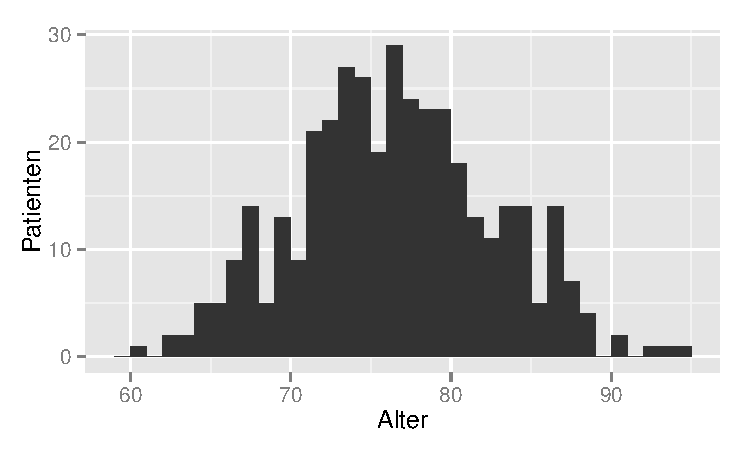
\includegraphics[width=\textwidth]{Grafiken/altersverteilung.pdf}
  \caption{Alter der untersuchten Patienten, Markierung bei 65 Jahren
    (interne Definition eines geriatrisch-onkologischen Patienten)}
  \label{fig:altersverteilung}
\end{figure}

Als Vergleich zeigt
Abbildung~\ref{fig:altersverteilungAllgemein} die
Altersverteilung aller in der onkologischen Klinik behandelten
Patienten aus den Jahren 2014 und 2015. \percentGeriatrischOnkologie{}\%
der Patienten waren 65 Jahre oder �lter.

\begin{figure}[htbp]
  \centering
  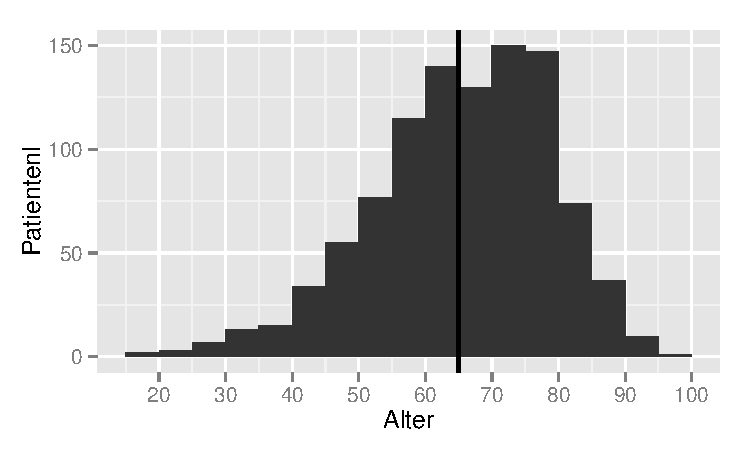
\includegraphics[width=\textwidth]{Grafiken/altersverteilungAllgemein.pdf}
  \caption{Alter aller Patienten der Klinik f�r internistische
    Onkologie der Jahre 2014 und 2015, Markierung bei 65 Jahren
    (interne Definition eines geriatrisch-onkologischen Patienten)}
  \label{fig:altersverteilungAllgemein}
\end{figure}

Die unterschiedlichen Diagnosen der untersuchten Patienten sind in
Abbildung~\ref{fig:diagnosen} gezeigt.

\begin{figure}[htbp]
  \centering
  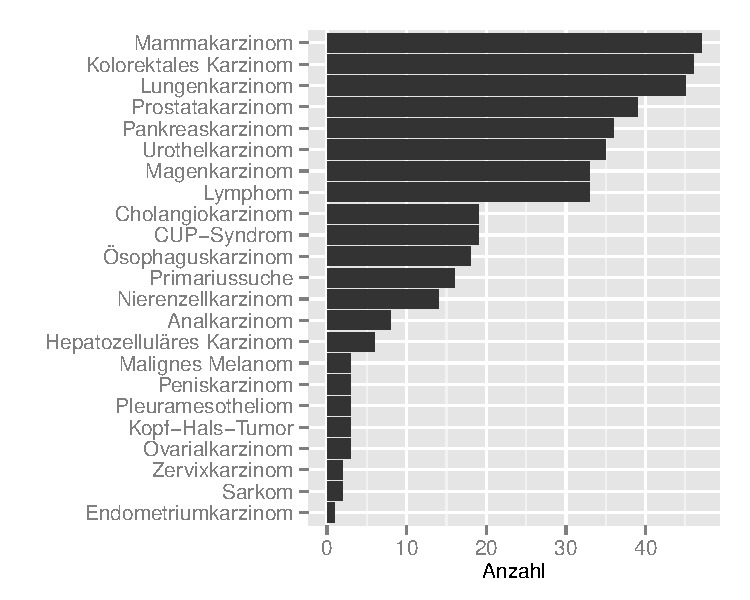
\includegraphics[width=\textwidth]{Grafiken/diagnosen.pdf}
  \caption{Diagnosen und H�ufigkeit der untersuchten Patienten}
  \label{fig:diagnosen}
\end{figure}

\section{Umfassendes Geriatrisches Assessment}

Eine Zusammenfassung der nachfolgend beschriebenen Ergebnisse ist in
Tabelle~\ref{tab:cga_summary} und in
Abbildung~\ref{fig:cga_summary_boxplot} dargestellt.

\begin{table}[htbp]
\caption{Zusammenfassung der erhobenen Daten innerhalb des
  Assessments}
\label{tab:cga_summary}
\centering
\begin{tabular}{lcccccc}
\toprule
& n & in \%*  &
  Minimum & Maximum & Median & IQR** \\ 
\midrule
Barthel-Index & 412 & 98 & 0 & 100 & 100 & 20 \\ 
IADL-Skala & 395 & 94 & 0 & 8 & 6 & 3 \\ 
Tinetti-Test & 400 & 95 & 0 & 28 & 24 & 11 \\ 
TUG-Test & 365 & 87 & 5 & 120 & 10 & 7,0 \\ 
MMS-Test & 374 & 89 & 11 & 30 & 29 & 3 \\ 
DemTect & 157 & 79*** & 0 & 18 & 13 & 7 \\ 
GDS & 115 & 91*** & 0 & 14 & 3 & 4 \\ 
DIA-Skala & 265 & 90*** & 0 & 10 & 2 & 3 \\ 
Charlson-Index & 399 & 95 & 0 & 9 & 1 & 2 \\ 
MNA & 358 & 85 & 8 & 28,5 & 22,0 & 6 \\ 
Sozial & 379 & 90 &  &  &  \\ 
\bottomrule
\multicolumn{7}{l}{*bezogen auf \nPatients{} Patienten,
  **IQR:~Interquartilsabstand,}\\
\multicolumn{7}{l}{***bezogen auf Zahl der Patienten bei denen dieser
  Test grunds�tzlich durch-}\\
\multicolumn{7}{l}{gef�hrt wurde (DemTect 200, GDS 126, DIA 295)}\\
\end{tabular}
\end{table}

\begin{figure}[htbp]
  \centering
  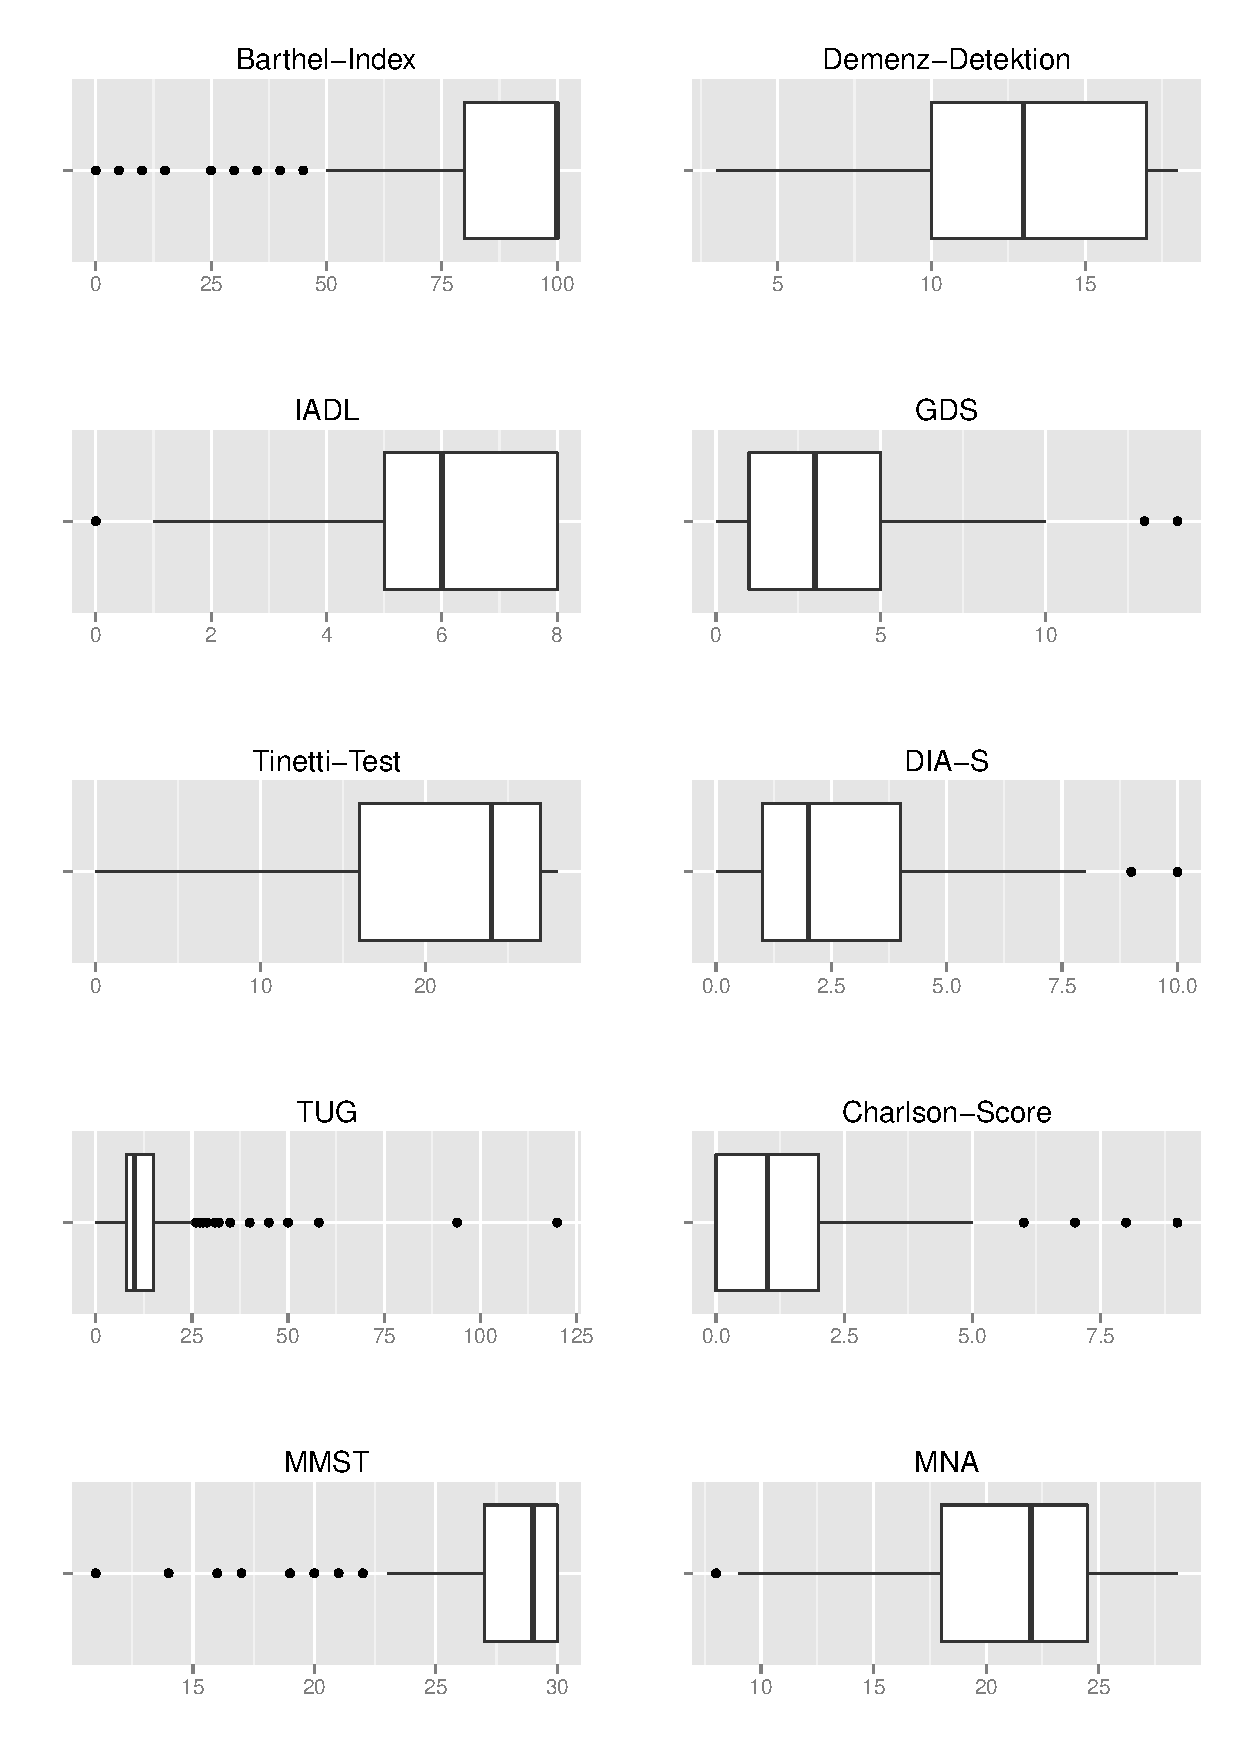
\includegraphics[width=\textwidth]{Grafiken/cga_summary_boxplot.pdf}
  \caption{Box-Whisker-Plot der einzelnen Tests des CGA, die Boxen
    bezeichnen den Abstand zwischen unterem und oberen Quartil mit dem
  innerhalb gelegenen Median, die durchgezogenen Linien umfassen
  jeweils noch den Datenpunkt, der innerhalb des anderthalbfachen IQR
  liegt, Ausrei�er sind als Punkte dargestellt}
  \label{fig:cga_summary_boxplot}
\end{figure}

\subsection{Barthel-Index}
Der Barthel-Index war bei \nBarthel{} Patienten
(\percentBarthel{}\%) verf�gbar. Den Maximalwert von
\barthelMax{}~Punkten erreichten \percentBarthelMax{}\% der
Patienten. Der Median lag bei \medianBarthel{}~Punkten.

\subsection{IADL-Skala}
Die IADL-Skala wurde bei \nIadl{} Patienten (\percentIadl{}\%)
angewandt. Den h�chsten Wert von \iadlMax{}~Punkten erreichten
\percentIadlMax{}\%. Der Median lag bei \medianIadl{}~Punkten.

\subsection{Tinetti-Test}
Der Tinetti-Test wurde bei \nTinetti{} Patienten (\percentTinetti{}\%)
durchgef�hrt. Den maximalen Wert von \tinettiMax{}~Punkten erreichten
\percentTinettiMax{}\% der Patienten. Der Median lag bei
\medianTinetti{}~Punkten. Nach der Einsch�tzung des Tinetti-Tests
besteht bei \percentTinettiModerateRisk{}\% der untersuchten Patienten
ein moderates Sturzrisiko ($19 \leq Tinetti \leq 24$), bei
\percentTinettiHighRisk{}\% ein hohes Sturzrisiko ($Tinetti \leq 18$).

\subsection{Timed Up And Go}
Der Timed-Up-And-Go-Test wurde bei \nTug{} Patienten
(\percentTug{}\%) durgef�hrt. Minimal wurden \tugMin{}~Sekunden
erreicht, maximal \tugMax{}~ Sekunden, bei \tugNotPossible{} Patienten
war die Durchf�hrung des Tests nicht m�glich. Die mediane Zeit zur
Bew�ltigung des Tests bei den Patienten, die teilnehmen konnten, lag
bei \medianTug{}~Sekunden. Nach Beurteilung des TUG besteht bei ...
Patienten eine eingeschr�nkte Mobilit�t, die jedoch noch zu keiner
Einschr�nkung im Alter f�hrt ($10 \leq TUG \leq 19$). Bei ... Patienten muss
von einer Beeintr�chtigung in den Aktivit�ten des t�glichen Lebens
ausgegangen werden ($ TUG \geq 20$).

\subsection{Mini-Mental-Status-Test}
Der MMST wurde bei \nMmst{} Patienten (\percentMmst{}\%)
durchgef�hrt. Nach der Unterteilung der aktuellen
deutschen S3-Leitlinie Demenz wird je nach Punktwert die in
Tabelle~\ref{tab:mmst} gezeigte Unterteilung vorgenommen. Daneben
zeigt die Tabelle den Anteil der untersuchten Patienten in der
jeweiligen Kategorie.

\begin{table}[htbp]
\caption{Einteilung einer Demenz nach MMST\autocite{LeitlinieDemenz2009}}
\label{tab:mmst}
\centering
\begin{tabular}{cccc}
\toprule
Schweregrad & MMST-Punktzahl & Patienten & Anteil in \%*\\
\midrule
keine Demenz& 27-30 & \nMmstNormal{} & \percentMmstNormal{}\\
Leicht & 20-26 & \nMmstLight{} & \percentMmstLight{}\\
Mittel & 10-19 & \nMmstModerate & \percentMmstModerate{}\\
Schwer & 0-9 & \nMmstSevere & \percentMmstSevere{}\\
\bottomrule
\multicolumn{4}{l}{*bezogen auf \nMmst{} Patienten}\\
\end{tabular}
\end{table}

\subsection{Demenz-Detektions-Test}
Seit Februar 2015 wurde zus�tzlich zum MMST der
Demenz-Detektions-Test, DemTect durchgef�hrt. Durchgef�hrt wurde der
DemTect bei \nDemtect{} Patienten (\percentDemtect\%, bezogen auf die
seit Februar 2015 untersuchten Patienten).
Ein normales Testergebnis ($Demtect \geq 13$) erreichten
\percentDemtectNormal{}\% der
Patienten, eine laut DemTect milde kognitive Beeintr�chtigung
($9 \leq Demtect \leq 12$) besteht bei \percentDemtectLight{}\% der Patienten. Bei
\percentDemtectDemenz{}\% der Patienten besteht laut DemTect eine
Demenz. Diese Ergebnisse fasst Tabelle \ref{tab:demtect} noch einmal
zusammen.

\begin{table}[htbp]
\caption{Demenz-Detektions-Test \autocite{Kalbe2004}}
\label{tab:demtect}
\centering
\begin{tabular}{cccc}
\toprule
Ergebnis & Punktzahl & Patienten & Anteil in \%*\\
\midrule
Normale kognitive Funktion & 13-18 & \nDemtectNormal{} & \percentDemtectNormal{}\\
Milde kognitive Beeintr�chtigung & 9-12 & \nDemtectLight{} & \percentDemtectLight{}\\
Demenz & 0-8 & \nDemtectDemenz{} & \percentDemtectDemenz{}\\
\bottomrule
\multicolumn{4}{l}{*bezogen auf insgesamt \nDemtect{} Patienten}\\
\end{tabular}
\end{table}

\subsection{Depressionsassessment}
Bis August 2014 wurde innerhalb des Assessments als
Depressionsscreening der GDS durchgef�hrt. Seit September 2014 dann
der DIA-Score. Diese Entscheidung wurde nicht aufgrund von Daten
gef�llt, sondern wegen der Durchf�hrbarkeit. In der Anwendung hat sich
der f�r geriatrische Patienten ohne Tumorerkrankung entwickelte GDS aufgrund der
verwendeten Fragen bei onkologischen Patienten als problematisch
erwiesen. Manche Fragen sind bei einer Tumorerkrankung so
offensichtlich mit ja zu beantworten, dass erstens die Befragung
schwerf�llt und zweitens auch die Auswertung fraglich erscheint. Daher
wurde ab September 2014 der in der Anwendung und Befragung besser
angenommene DIA-Score verwendet.

\subsubsection{GDS}
Der GDS wurde bei \nGds{} Patienten (\percentGds{}\%, bezogen auf die
bis August 2014 untersuchten Patienten) bestimmt. Der
maximal bestimmt Wert betrug \gdsMax{}, der mininmal bestimmte
\gdsMin{}. Nach Einteilung des GDS ist ein Wert bis 5 normale
einzusch�tzen, zwichen 6 und 9 besteht der Verdacht auf eine
Depression und weitere Diagnostik sollte angestrebt werden, ab einem
Wert von 10 besteht fast immer auch eine Depression. Nach dieser
Einteilung wurden \percentGdsNormal{}\% der Patienten als normal
eingesch�tzt, bei \percentGdsSuspect{}\% bestand der Verdacht auf eine
Depression, und \percentGdsDepression{}\% hatten laut GDS-Einteilung
fast sicher eine Depression.

\subsubsection{DIA-Skala}
Dia DIA-Skala kam bei \nDia{} Patienten (\percentDia{}\%, bezogen auf die
ab September 2014 untersuchten Patienten) zur Anwendung. Maximal wurde
ein Wert von 10 bestimmt. In der Skala des Tests ist ein Wert bis zwei
normal. Bei einem Wert von 3 besteht Depressionsverdacht und ab einem
Wert von 4 ist ein Depression von Krankheitswert wahrscheinlich. Nach
dieser Einteilung hatten \percentDiaNormal{}\% der Patienten einen
unauff�lliges Testergebnis. Bei \percentDiaSuspect{}\% besteht
Depressionsverdacht und bei \percentDiaDepression{}\% der Patienten
ist eine Depression von Krankheitswert laut DIA-S wahrscheinlich. 

\subsection{Komorbidit�t}
Der Charlson-Komorbidit�tsindex stand bei \nCharlson{} Patienten
(\percentCharlson{}\%) zur Verf�gung. \percentCharlsonZero{}\% der
Patienten wiesen keine relevante Komorbidit�t auf, hatten also ein
Charlson-Index von 0. Drei oder mehr relevante Komorbit�ten hatten
\percentCharlsonThreeOrMore{}\% der Patienten.

\subsection{Ern�hrungsstatus}
Der Ernh�hrungsstatus wurde mittels MNA bei \nMna{} Patienten
(\percentMna{}\%) durchgef�hrt. Die einzelnen Grenzwerte und
Kategorien laut MNA sowie der Anteil der Patienten in der jeweiligen
Kategorie sind in Tabelle~\ref{tab:mna} zusammengefasst.

\begin{table}[htbp]
\caption{Mini Nutritional Assessment \autocite{Guigoz1997}}
\label{tab:mna}
\centering
\begin{tabular}{cccc}
\toprule
Ern�hrungsstatus & MNA-Punktzahl & Patienten & Anteil in \%*\\
\midrule
Unauff�llig & $ \geq 24 $ & \nMnaNormal{} & \mnaNormal{}\\
Risiko f�r Unterern�hrung & 17 bis 23,5 & \nMnaRisk{} & \mnaRisk{}\\
Unterern�hrung & > 17 & \nMnaMalnourished{} & \mnaMalnourished{}\\
\bottomrule
\multicolumn{4}{l}{*bezogen auf insgesamt \nMna{} Patienten}\\
\end{tabular}
\end{table}

\subsection{Soziale Situation}
Ein Sozialassessment wurde bei \nSocialStatus{} Patienten
(\percentSocialStatus{}\%) durchgef�hrt. Wie in
Abschnitt~\ref{sec:sozial} beschrieben wurde aus dem rein
beschreibenden Text eine kategorielle Variable Alleinlebend erstellt,
die die Werte wahr oder falsch annehmen kann. Laut Assessment waren
\percentSocialAlone{}\% der untersuchten Patienten alleinlebend.

\subsection{Anzahl der Defizite im Assessment}
\label{sec:defizite}

In Anlehnung an die Definition von Wedding et. al
\autocite{Wedding2007} wurden
die Ergebnisse des Barthel-Index, der IADL-Skala, des MNA, der MMSE
und des DemTect-Tests, des Komorbidit�tsindex und des Tinetti-Tests
benutzt,
um die Anzahl der Defizite zu berechnen. Dabei wurde anders als in der
angegebenen Publikation jedes auf�llige Testergebniss als Defizit
definiert, also Barthel-Index kleiner 100, IADL-Wert kleiner 7, MNA kleiner
24, MMSE kleiner 27 oder DemTect kleiner 13, Charlson-Index gr��er 0
und Tinetti-Test kleiner 25. Zur Diskussion und Erkl�rung der
Abweichung siehe Abschnitt~\ref{sec:defizite_discussion}.
Bei 297 Patienten liegen alle ben�tigten Werte vor (71\%), der Median
liegt bei 2 Defiziten, die
H�ufigkeitsverteilung ist in Tabelle~\ref{tab:defizite} gezeigt.

\begin{table}[htbp]
\caption{Anzahl der Defizite im Assessment}
\label{tab:defizite}
\centering
\begin{tabular}{ccc}
\toprule
Anzahl der Defizite & Patienten & Anteil in \%*\\
\midrule
0 & 35 & 12 \\
1 & 61 & 21 \\
2 & 58 & 20 \\
3 & 45 & 15 \\
4 & 40 & 13 \\
5 & 39 & 13 \\
6 & 19 & 6 \\
\bottomrule
\multicolumn{3}{l}{*bezogen auf insgesamt 297 Patienten}\\
\end{tabular}
\end{table}

\subsection{Korrelation}

In Tabelle~\ref{tab:correlation} sind die Korrelationskoeffizienten
nach Spearman zwischen den einzelnen Assessmenttests mit ihrem
Standardfehler (siehe Gleichung~\ref{eq:spearman})
aufgef�hrt. Ber�cksichtigt wurden Korrelationen gr��er als 0,4;
sortiert wurde nach abnehmender Korrelation.

\begin{table}[htbp]
\caption{Rangkorrelationskoeffizienten}
\label{tab:correlation}
\centering
\begin{tabular}{lclcc}
\toprule
\multicolumn{3}{c}{Kategorien} & Koeffizient $\rho$ & Standardfehler $\sigma$\\
\midrule
Tinetti& -& TUG & -0,86 & 0,03 \\
Tinetti& -& Barthel & 0,73 & 0,03 \\
DemTect& -& MMST & 0,65 & 0,05 \\
TUG& -& Barthel & -0,63  & 0,03 \\
Tinetti& -& IADL & 0,52 & 0,03 \\
GDS& -& IADL & -0,51 & 0,06 \\
BMI& -& MNA & 0,50 & 0,03 \\
IADL& -& Barthel & 0,48 & 0,03 \\
IADL&-& TUG &-0,47 & 0,03 \\
MNA& -& Barthel & 0,47 & 0,03 \\
MNA& - & Tinetti & 0,41 & 0,03\\
\bottomrule
\end{tabular}
\end{table}

\section{Einsch�tzungsm�glichkeiten der Behandlungsf�higkeit}

In der Vergangenheit kamen einige onkologische Behandlungen allein
aufgrund des Alters f�r einige Patienten nicht in Frage. Daher wurde
f�r die folgenden Darstellung der Ergebnisse des Assessments in
Abh�ngigkeit von der Einteilung durch die verschiedenen
Einsch�tzungsm�glichkeiten (Einteilung nach Balducci, Einteilung durch
pers�nliche Einsch�tzung des Behandlers und Einteilung durch
Konferenzbeschluss), auch eine Unterteilung durch verschieden
Altersgruppen mit aufgenommen. Tabelle~\ref{tab:classification} stellt
die relativen H�ufigkeiten der einzelnen Kategorien dar. In den
folgenden Tabellen, die die Ergebnisse des Assessments darstellen
wurden dann auch die absoluten H�ufigkeiten mit angegeben.

\begin{table}[htbp]
\caption{Relative H�ufigkeiten der einzelnen Kategorien verschiedener
  Einsch�tzungsm�glichkeiten}
\label{tab:classification}
\centering
\begin{tabular}{lcccc}
\toprule
&\multicolumn{3}{c}{Anteil der Patienten in \%} & Vollst�ndigkeit in \% \\
Einsch�tzungsm�glichkeit & no go & slow go & go go & von 421 Patienten\\
\midrule
Pers�nliche Einsch�tzung & 12 & 41 & 46 & 85 \\
Einteilung nach Balducci & 55 & 30 & 15 & 88 \\
Konferenzeinsch�tzung    & 15 & 38 & 47 & 93 \\
Alter*                   & 9  & 50 & 41 & 97 \\
\bottomrule
\multicolumn{5}{l}{*no go entspricht den 85 bis 94 j�hrigen, slow go den 75 bis
  84 j�hrigen und}\\
\multicolumn{5}{l}{go go den 65 bis 74 j�hrigen}\\
\end{tabular}
\end{table}

\subsection{Alter}
Tabelle~\ref{tab:cga_alter} zeigt die Mediane der erhobenen Parameter des
Assessments f�r die verschiedenen Altersgruppen. Zur Signifikanztestung der
beobachteten Unterschiede kam der
Kruskal-Wallis-Test zur Anwendung. Eine post-hoc-Analyse mittels
Wilcoxon-Rangsummentest und p-Wert Korrektur mittels
Bonferroni-Methode wurde bei signifikantem Kruskal-Wallis-Test
durchgef�hrt (siehe~\ref{subsec:Signifikanztests}).

\begin{table}[htbp]
\caption{Medianwerte der erhobenen Daten innerhalb des umfassenden
  geriatrischen Assessments nach verschiedenen Altersgruppen}
\label{tab:cga_alter}
\centering
\begin{tabular}{lccccc}
  \toprule
  &\multicolumn{3}{c}{Altersgruppe}\\
  & A & B & C & & Signifikanz** \\
  & 65 bis 74 & 75 bis 84 & 85 bis 94 & p-Wert* & Gruppenvergleich \\
  \midrule
  Patienten & 168 & 205 & 36 &\\ 
  Barthel-Index & 100 & 95 & 85 & <0,001 & AB, AC\\ 
  IADL-Skala & 7 & 6 & 5 & 0,001 & AC, BC\\
  Tinetti-Test & 26 & 23 & 16 & <0,001 & AB, AC, BC\\ 
  TUG-Test & 8 & 10 & 12 & <0,001 & AB, AC\\ 
  MMS-Test & 29 & 28 & 27 & 0,002 & AB, AC\\ 
  DemTect & 14,0 & 13,0 & 8,5 & <0,001 & AC, BC\\ 
  GDS & 2 & 2 & 6 & 0,08 \\ 
  DIA-Skala & 20 & 2 & 2 & 0,6\\ 
  Charlson-Index & 1 & 1 & 1 & 0,1\\ 
  MNA & 22 & 22 & 22 & 0,6\\ 
  Alleinlebend & 24\% & 35\% & 24\% & 0,2***\\
  Defizite & 2 & 3 & 3 & <0,001 & AB, AC\\
  \bottomrule
\multicolumn{6}{l}{*Kruskal-Wallis-Test, **Wilcoxon-Rangsummentest, ***$\chi^2$-Test}\\
\end{tabular}
\end{table}

\begin{table}[htbp]
\caption{Medianwerte der erhobenen Daten innerhalb des umfassenden
  geriatrischen Assessments nach Unterteilung durch Balducci}
\label{tab:cga_balducci}
\centering
\begin{tabular}{lccccc}
  \toprule
  &\multicolumn{3}{c}{Einteilung durch Balducci}\\
  & A & B & C & & Signifikanz** \\
  & no go & slow go & go go & p-Wert* &Gruppenvergleich \\
  \midrule
  Patienten & 205 & 111 & 55 &\\ 
  Barthel-Index & 85 & 100  & 100 & <0,001*** & AB, AC\\ 
  IADL-Skala & 5 & 6 & 8 & <0,001*** & AB, AC, BC\\
  Tinetti-Test & 18& 26 & 28 & <0,001 & AB, AC\\ 
  TUG-Test & 12 & 8  & 7 & <0,001 &AB, AC, BC\\ 
  MMS-Test & 28 & 29 & 30 & <0,001 & AB, AC\\ 
  DemTect & 13 & 14  & 16  & <0,001 &AB, AC\\ 
  GDS & 3,0 & 3,0 & 1,5 & 0,002& AC, BC\\ 
  DIA-Skala & 3 & 2   & 1   & 0,026 & AC\\ 
  Charlson-Index & 2 & 1 & 0 & <0,001*** &AB, AC, BC\\ 
  MNA & 20   & 23   & 24   & <0,001&AB, AC\\ 
  Alleinlebend & 30\% & 23\% & 31\% & 0,3****\\
  Defizite & 4 & 2 & 1 & <0,001 & AB, AC, BC\\
  \bottomrule
\multicolumn{6}{l}{*Kruskal-Wallis-Test, ** Wilcoxon-Rangsummentest
  mit Gruppe A: no go,}\\
\multicolumn{6}{l}{Gruppe B: slow go, Gruppe C: go go, *** nicht
  aussagekr�ftig, da Kriterium}\\
\multicolumn{6}{l}{zur Einteilung, ****$\chi^2$-Test}\\
\end{tabular}
\end{table}

\begin{table}[htbp]
\caption{Medianwerte der erhobenen Daten innerhalb des umfassenden
  geriatrischen Assessments nach Einsch�tzung des Behandlers}
\label{tab:cga_personal}
\centering
\begin{tabular}{lccccc}
  \toprule
  &\multicolumn{3}{c}{Einsch�tzung des Behandlers}\\
  & A & B & C & & Signifikanz** \\
  & no go & slow go & go go & p-Wert* &Gruppenvergleich \\
  \midrule
  Patienten & 44 & 147 & 165&\\ 
  Barthel-Index & 45 & 95 & 100 & <0,001 & AB, AC, BC\\ 
  IADL-Skala & 3 & 6 & 8 & <0,001 & AB, AC, BC\\
  Tinetti-Test & 7 & 21 & 27 & <0,001 & AB, AC, BC\\ 
  TUG-Test & 20 & 12 & 8 & <0,001 & AB, AC, BC\\ 
  MMS-Test & 25 & 28 & 29 & <0,001 &AB, AC, BC\\ 
  DemTect & 8& 13& 15& <0,001 & AB, AC, BC\\ 
  GDS & NA*** & 4 & 2 & 0,02 & zu geringes n\\ 
  DIA-Skala & 4 & 3  & 1  & <0,001 & AC, BC\\ 
  Charlson-Index & 2,5& 2,0 & 0 & <0,001 & AB, AC, BC\\ 
  MNA & 16,0  & 20,5  & 24,0   & <0,001 & AB, AC, BC\\ 
  Alleinlebend & 32\% & 32\% & 24\% & 0,2****\\
  Defizite & 5 & 3 & 1 & <0,001 & AB, AC, BC\\
  \bottomrule
\multicolumn{6}{l}{*Kruskal-Wallis-Test, **Wilcoxon-Rangsummentest mit
  Gruppe A: no go,}\\
\multicolumn{6}{l}{Gruppe B: slow go, Gruppe C: go go, ***nicht
  vorhanden, ****$\chi^2$-Test}\\
\end{tabular}
\end{table}

\begin{table}[htbp]
\caption{Medianwerte der erhobenen Daten innerhalb des umfassenden
  geriatrischen Assessments nach Unterteilung durch die Konferenz}
\label{tab:cga_konferenz}
\centering
\begin{tabular}{lccccc}
  \toprule
  &\multicolumn{3}{c}{Einteilung durch Konferenz}\\
  & A & B & C & & Signifikanz** \\
  & no go & slow go & go go & p-Wert* &Gruppenvergleich \\
  \midrule
  Patienten & 59  & 150 & 183&\\ 
  Barthel-Index & 50 & 90   & 100 & <0,001& AB, AC, BC\\ 
  IADL-Skala & 3 & 6 & 8 & <0,001& AB, AC, BC\\
  Tinetti-Test & 10& 21 & 27 & <0,001& AB, AC, BC\\ 
  TUG-Test & 20 & 12 & 8 & <0,001& AB, AC, BC\\ 
  MMS-Test & 25 & 28 & 29 & <0,001& AB, AC, BC\\ 
  DemTect & 9 & 13  & 16  & <0,001& AB, AC, BC\\ 
  GDS & 8& 4 & 2 & <0,001& BC\\ 
  DIA-Skala & 4 & 2   & 2   & 0,002&AC\\ 
  Charlson-Index & 2 & 2 & 1 & <0,001 & AC, BC\\ 
  MNA & 17   & 21   & 24   & <0,001& AB, AC, BC\\ 
  Alleinlebend & 29\% & 33\% & 22\% & 0,05*** & BC*** \\
  Defizite & 5 & 3 & 1 & <0,001 & AB, AC, BC\\
  \bottomrule
\multicolumn{6}{l}{*Kruskal-Wallis-Test, **Wilcoxon-Rangsummentest mit
  Gruppe A: no go,}\\
\multicolumn{6}{l}{Gruppe B: slow go, Gruppe C: go go, ***$\chi^2$-Test}\\
\end{tabular}
\end{table}

\subsection{Einteilung nach Vorschlag von Balducci}
In der von Balducci vorgeschlagenen Einteilung
\autocite{Balducci2000} werden der Barthel-Index, der IADL-Wert und der
Charlson-Komorbidit�tsindex ber�cksichtigt (Tabelle
\ref{tab:balducci}). Danach k�nnen anhand der vorliegenden Daten
\nBalducci{} Patienten (\percentBalducci{}\%) beurteilt werden.
Von Balducci werden f�r die unterteilten Kategorien die Begriffe
gebrechlich (frail), gef�hrdet (vulnerable) und fit (fit)
verwendet. Die jeweiligen Definitionen decken sich mit
den hier verwendeten Kategorien uneingeschr�nkt behandlungsf�hig, eingeschr�nkt
behandlungsf�hig und nicht behandlungsf�hig.
\percentBalducciNogo{}\% der Patienten sind nach der Einteilung von Balducci 
nicht therapief�hig, \percentBalducciSlowgo{}\% eingeschr�nkt
therapief�hig und \percentBalducciGogo{}\% uneingeschr�nkt
therapief�hig.

Tabelle~\ref{tab:cga_balducci} zeigt die Medianwerte der erhobenen Parameter des
Assessments f�r die verschiedenen Gruppen, nach Einteilung durch den
Vorschlag von Balducci.

\subsection{Einteilung nach Einsch�tzung des Behandlers}
Eine Einsch�tzung des behandelnden Onkologen lag bei \nPersonal{}
Patienten (\percentPersonal{}\% bezogen auf die seit der Einf�hrung
der Befragung im April 2014 besprochenen Patienten) vor. Danach wurden
\percentPersonalGogo{}\% der Patienten als uneingeschr�nkt
behandlungsf�hig eingesch�tzt, \percentPersonalSlowgo{}\% als
eingeschr�nkt behandlungsf�hig und \percentPersonalNogo{}\% als nicht
behandlungsf�hig.

Tabelle~\ref{tab:cga_personal} zeigt die Mediane der erhobenen Parameter des
Assessments f�r die verschiedenen Gruppen, nach Einteilung durch die
Einsch�tzung des Behandlers.

\subsection{Einteilung nach Konferenzbeschluss}
\nPatients{} Patienten wurden
von \ersterPatient{} bis \letzterPatient{} in der
geria\-trisch"=onkolo\-gischen
Konferenz besprochen. Bei \nKonferenz{} Patienten
(\percentKonferenz{}\%) kam ein
Konferenzbeschluss zustande. \percentKonferenzNogo{}\% der beurteilten
Patienten wurden als
nicht therapief�hig eingesch�tzt, \percentKonferenzSlowgo{}\% der
Patienten als eingeschr�nkt therapief�hig und \percentKonferenzGogo{}\%
der Patienten als uneingeschr�nkt therapief�hig. Bei \nKonferenzNa{}
Patienten kam kein Konferenzbeschluss zustande. Daf�r gab es
verschiedene Gr�nde. Zum Beispiel waren einige Patienten zum Zeitpunkt
der Konferenz bereits verstorben. Einzelne Assessments waren so
unvollst�ndig, dass eine Einsch�tzung nicht m�glich war. Einzelne
Patienten wurden aufgrund des
Alters unter 65 Jahre und fehlender spezifischer Probleme als nicht
geriatrisch klassifiziert. Bei drei Patienten aus den Anf�ngen der
Konferenz wurde als Beschluss
eine Therapie empfohlen, jedoch keine Angabe zur eingesch�tzten
Behandlungsf�higkeit gegeben.

\begin{figure}[htbp]
  \centering
  \includegraphics[width=\textwidth]{Grafiken/beschlussverteilung.pdf}
  \caption{Alter der untersuchten Patienten, aufgeteilt nach
    Konferenzbeschluss, no\_go, slow\_go und go\_go entspricht nicht,
    eingeschr�nkt und uneingeschr�nkt therapief�hig, NA bedeutet, dass
    kein Konferenzbeschluss vorliegt}
  \label{fig:beschlussverteilung}
\end{figure}

Tabelle~\ref{tab:cga_konferenz} zeigt die Medianwerte der erhobenen Parameter des
Assessments f�r die verschiedenen Gruppen, nach Einteilung durch die
geria\-trisch"=onkolo\-gische Konferenz.

Abbildung~\ref{fig:beschlussverteilung} zeigt die Altersverteilung der
Patienten jeder einzelnen Kategorie des Konferenzbeschlusses.

Abbildung~\ref{fig:cga_konferenz} stellt die Ergebnisse der einzelnen
Assessmenttests f�r die Aufteilung nach Konferenzbeschluss grafisch dar.

\begin{figure}[htbp]
  \centering
  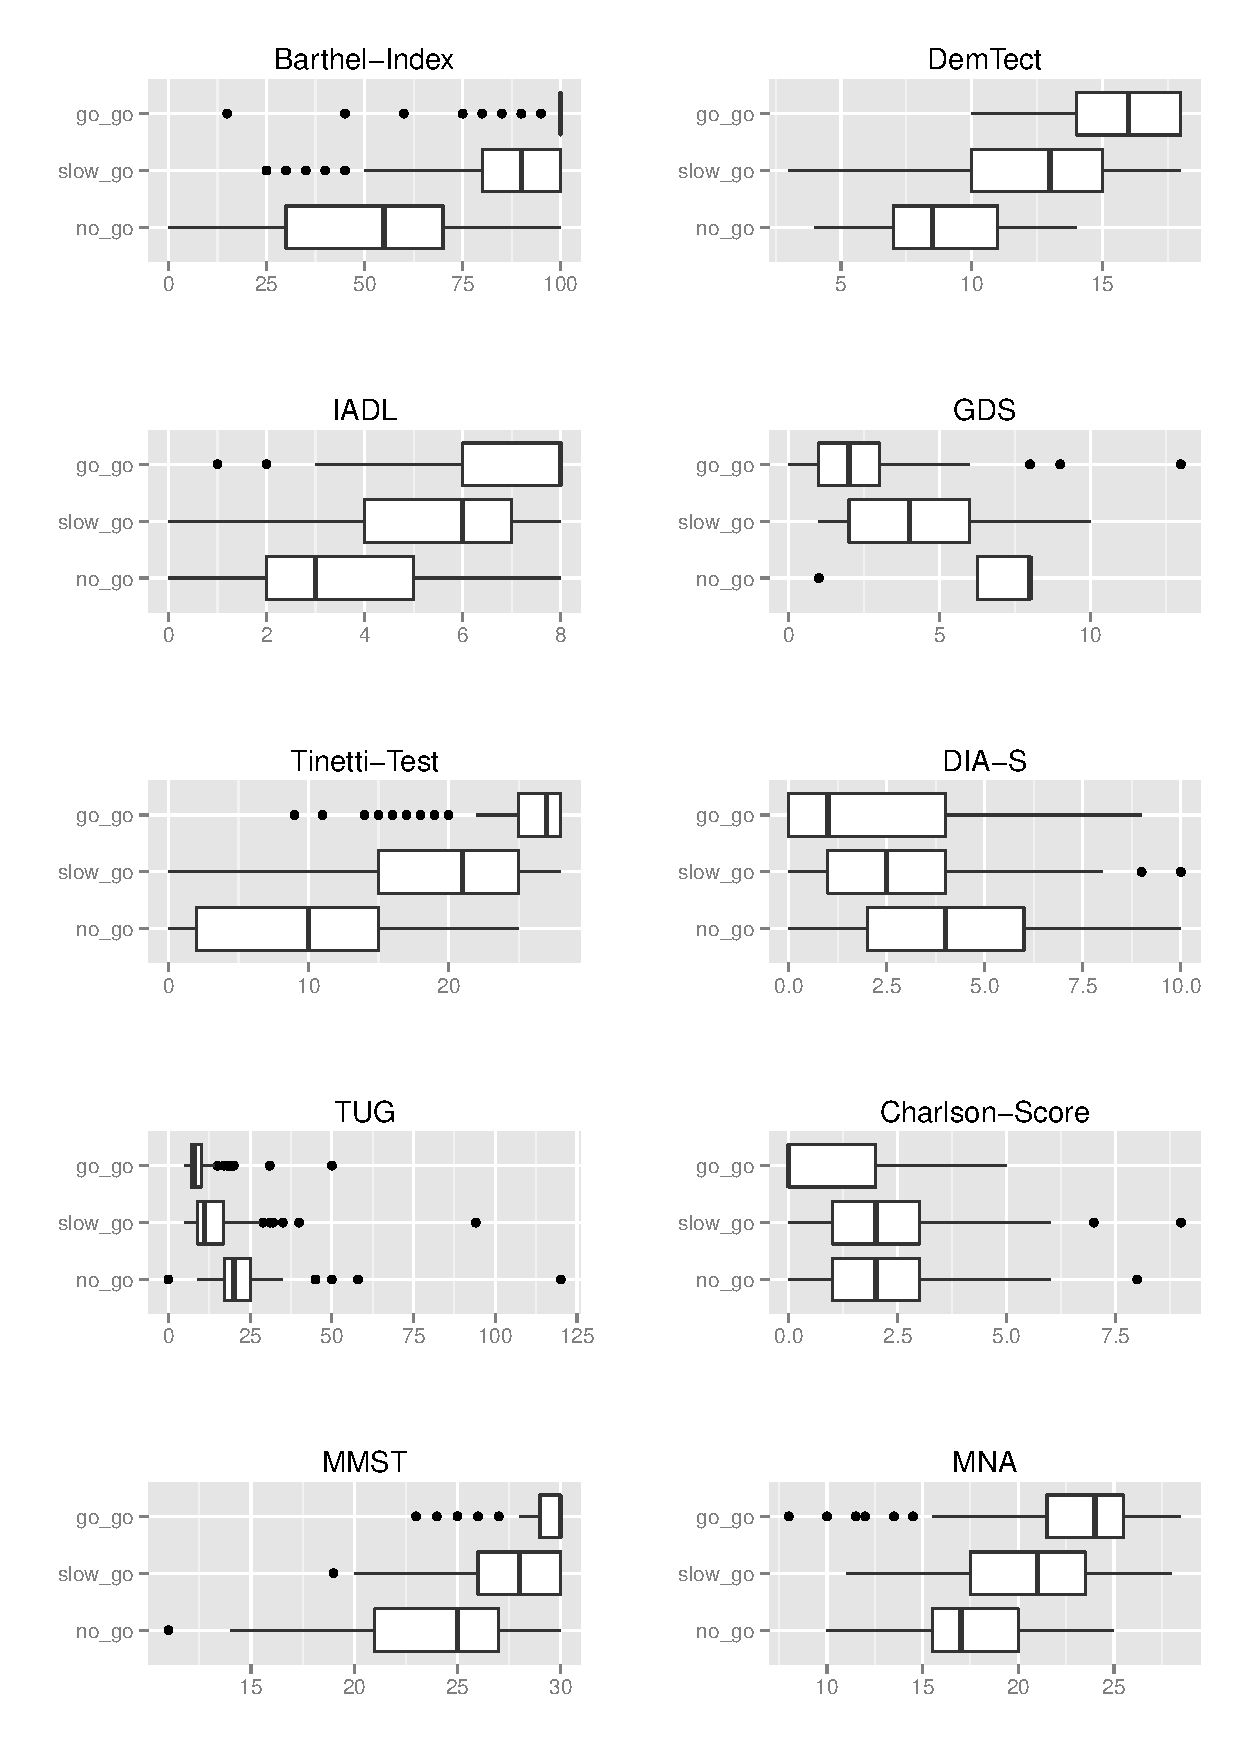
\includegraphics[width=\textwidth]{Grafiken/cga_konferenz.pdf}
  \caption{Box-Whisker-Plot der einzelnen Tests des CGA aufgeteilt nach
    Konferenzbeschluss, die Kasten bezeichnen den Abstand zwischen
    unterem  und oberen Quartil mit dem innerhalb gelegenen Median,
    die durchgezogenen Linien umfassen jeweils noch den Datenpunkt,
    der innerhalb des anderthalbfachen IQR liegt, Ausrei�er sind als
    Punkte dargestellt}
  \label{fig:cga_konferenz}
\end{figure}

\subsection{Vergleich der unterschiedlichen Verfahren zur Einsch�tzung
  der Therapief�higkeit}

\subsubsection{Einsch�tzung des Behandlers und Einteilung nach
  Konferenzbeschluss}

Tabelle~\ref{tab:konferenz_personal} zeigt die Kontingenztafel der
Einsch�tzung des Behandlers und des Konferenzbeschlusses. F�r
\nKonferenzPersonal{} Patienten standen beide Beurteilungen zur
Verf�gung.

Ein Blick auf die Tabelle gen�gt, um eine Unabh�ngigkeit
der Einsch�tzung des Behandlers und des Konferenzbeschlusses
auszuschlie�en. Die formale statistische Behandlung
(Abschnitt~\ref{subsec:Signifikanztests}) erfordert die
Durchf�hrung eines $\chi^2$-Tests. Dieser ergibt ein $\chi^2$ von 400 und
damit ein signifikantes Ergebnis (p<0,001). Zur Beurteilung der G�te
der �bereinstimmung kommt Cohens gewichtetes Kappa ($\kappa = 0,83$) zum
Einsatz. Anschaulicher ist der Anteil an �bereinstimmung mit
\percentAgreementKP{}\% der F�lle.

\begin{table}[htbp]
\caption{Vergleich der prim�ren Einsch�tzung des Behandlers und der Einteilung
  nach Konferenzbeschluss}
\label{tab:konferenz_personal}
\centering
\begin{tabular}{crrr}
  \toprule
  n=337              & \multicolumn{3}{c}{Einsch�tzung des Behandlers}\\
  Konferenzbeschluss & no go & slow go & go go \\ 
  \midrule
  no go              &  42   &  11     &   1   \\ 
  slow go            &   1   &  104    &  20   \\ 
  go go              &   0   &  23     & 135   \\ 
  \bottomrule
\end{tabular}
\end{table}

Abbildung~\ref{fig:konferenz_personal} stellt die einzelnen
Abweichungen grafisch dar, jeder Punkt entspricht einem Patienten.

\begin{figure}[htbp]
  \centering
  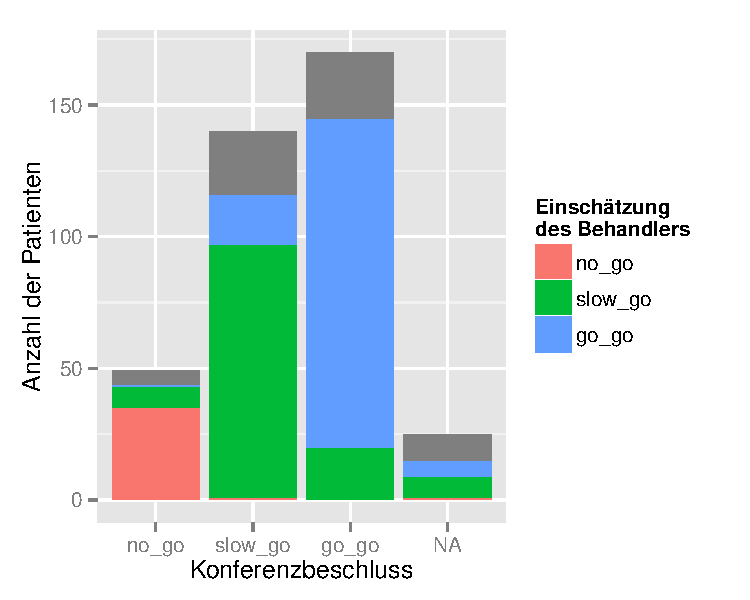
\includegraphics[width=\textwidth]{Grafiken/konferenz_personal.pdf}
  \caption{Grafische Darstellung der pers�nlichen Einsch�tzung des
    Behandlers und des Konferenzbeschlusses}
  \label{fig:konferenz_personal}
\end{figure}

\subsubsection{Einsch�tzung des Behandlers und Einteilung nach Vorschlag
  von Balducci}

Tabelle~\ref{tab:personal_balducci} zeigt mit Hilfe einer
Kontingenztafel Gemeinsamkeiten und Unterschiede der Einsch�tzung des
Behandlers und der Einteilung nach dem Vorschlag von Balducci.
F�r \nBalducciPersonal{} Patienten standen
beide Beurteilungen zur Verf�gung.

\begin{table}[htbp]
\caption{Vergleich der prim�ren Einsch�tzung des Behandlers
  und der Einteilung nach dem Vorschlag von Balducci}
\label{tab:personal_balducci}
\centering
\begin{tabular}{crrr}
  \toprule
  n=322&\multicolumn{3}{c}{Einsch�tzung des Behandlers}\\
  nach Balducci&no go&slow go&go go\\ 
  \midrule
  no go& 36 & 97 & 42 \\ 
  slow go & 0 & 31 & 68\\ 
  go go& 0 & 6 & 42 \\ 
  \bottomrule
\end{tabular}
\end{table}

Auch hier kann eine Unabh�ngigkeit der Einsch�tzung des Behandlers und
der Einteilung nach dem Vorschlag von Balducci ausgeschlossen
werden. Das $\chi^2$ betr�gt 100 und ist somit ebenfalls signifikant
(p<0,001). Cohens gewichtetes Kappa betr�gt $\kappa = 0,33$.
Es bestand �bereinstimmung in \percentAgreementBP{}\% der F�lle.

\subsubsection{Einteilung nach Vorschlag von Balducci und nach
  Konferenzbeschluss}

Tabelle~\ref{tab:konferenz_balducci} zeigt die Kontingenztafel der
Einteilung nach dem Vorschlag von Balducci und dem Konferenzbeschluss.
Beide Klassifikationen lagen in \nBalducciKonferenz{} F�llen vor.

\begin{table}[htbp]
\caption{Vergleich der Einteilung nach dem Vorschlag von
  Balducci und der Einteilung nach Konferenzbeschluss}
\label{tab:konferenz_balducci}
\centering
\begin{tabular}{crrr}
  \toprule
  n=359              & \multicolumn{3}{c}{Konferenzbeschluss}\\
  nach Balducci      & no go & slow go & go go \\ 
  \midrule
  no go              &  48   &  97     &  42   \\ 
  slow go            &   1   &  29     &  71   \\ 
  go go              &   0   &   3     &  47   \\ 
  \bottomrule
\end{tabular}
\end{table} 

Auch hier kann eine Unabh�ngigkeit der Einsch�tzung des Behandlers und
der Einteilung nach dem Vorschlag von Balducci ausgeschlossen
werden. Das $\chi^2$ betr�gt 100 und ist somit ebenfalls signifikant
(p<0,001). Cohens gewichtetes Kappa betr�gt $\kappa = 0,36$.
Es zeigte sich eine �bereinstimmung von \percentAgreementBK{}\% der
F�lle. 

\section{Statistisches Modell der Konferenzentscheidung}

\subsection{Erkl�rendes Modell}

Um den Effekt verschiedener Pr�diktoren vergleichen zu k�nnen, wurden die
Pr�diktoren nach Gleichung~\ref{eq:scale} auf die standardisierte
Zufallsvariable $Z$ normiert. Dabei sei $X$ die
Zufallsvariable eines Pr�diktors mit Erwartungswert $E(X) = \mu$ und
Varianz $Var(X) = \sigma^2$ also dementsprechend Standardabweichung $\sigma$.

\begin{equation}
\label{eq:scale}
Z = \frac{X-\mu}{\sigma}
\end{equation}

Genau genommen muss dabei von einer Studentisierung (nach dem
Pseudonym "`Student"' des Statistikers William Gosset) gesprochen
werden, da die genaue Verteilungsfunktion der Pr�diktoren nicht
bekannt ist. Daher wird statt des Erwartungswertes das arithmetische
Mittel und statt der Varianz die Stichprobenvarianz verwendet.

\subsubsection{Therapief�higkeit}

Als erstes stellt sich die Frage, welche Pr�diktoren die
Einteilung in nicht therapief�hig und therapief�hige Patienten am
besten erkl�rt. Gleichung~\ref{eq:logistic1} zeigt die logistische
Regression der dargestellten Situation. Dabei entspricht $P(Y=1|X_1 \land
X_2)$ der Wahrscheinlichkeit der Kategorie nicht behandlungsf�hig
und $X_1, X_2$ den Koeffizienten der Pr�diktoren Barthel-Index und
Ergebnis des MMST. $\epsilon$ bezeichnet den Fehler.

\begin{equation}
\label{eq:logistic1}
\text{logit}(P(no\_go)) = \beta_0 + \beta_1 X_1 + \beta_2 X_2 + \epsilon
\end{equation}

Die Pr�diktoren wurden von Hand ausgew�hlt. Dabei wurde zuerst eine
univariate logistische Regression f�r jeden erhobenen Parameter
durchgef�hrt und
anhand des p-Wertes der Einfluss des Parameters und anhand des AIC
(Akaike information criterion) die
G�te der Regression beurteilt. Da es sich in diesem Schritt um eine
beschreibendes Modell handelt wurden alle vorhandenen vollst�ndigen
Datens�tze zur Regression benutzt. Auch Polynome der Parameter h�herer
Ordnungen wurden untersucht. In einem zweiten Schritt wurden dann in
einer multivariaten Analyse
Kombinationen von Parametern inklusive deren Polynome und auch
Interaktionen getestet. Dabei schnitten der Barthel-Index, der Wert des
MMST und der IADL-Wert am besten ab. In dieser Dreierkombination ohne
h�hergradige Polynome und Interaktionen resultierte das beste
Modell, gemessen am AIC. Wegen der hohen Kolinearit�t des IADL-Wertes und des
Barthel-Index wurde der IADL-Wert letztendlich im endg�ltigen Modell
weggelassen (siehe Tabelle~\ref{tab:correlation},
Korrelationskoeffizient von 0.48). Eine hohe Kolinearit�t macht die
Interpretation des Modells schwieriger, da die einzelnen Effekte dann nicht
voneinander zu differenzieren sind. Die Regressionskoeffizienten
inklusive Standardfehler und p-Wert sind in
Tabelle~\ref{tab:logistic1} zusammengefasst.

\begin{table}[htbp]
\caption{Logistische Regression der Therapief�higkeit}
\label{tab:logistic1}
\centering
\begin{tabular}{lccr}
\toprule
Koeffizient (Pr�diktor)& Sch�tzwert & Standardfehler & p-Wert\\
\midrule
$\beta_0$ (Achsenabschnitt) & -2,97 & 0,31\\
$\beta_1$ (Barthel) & -1,65 & 0,24 & <0,001\\
$\beta_2$ (MMST) & -0,99 & 0,21 & <0,001\\
\bottomrule
\multicolumn{4}{l}{AIC (Akaikes Informationskriterium) 134, n=358}
\end{tabular}
\end{table}

Da die Parameter normiert sind, spiegelt die H�he des Koeffizienten
den Einfluss des Parameters wieder. Es zeigt sich also, dass der
Barthel-Index den h�chsten Einfluss besitzt und dass beide Parameter
mit abnehmenden Werten die Wahrscheinlichkeit der Kategorie nicht
behandlungsf�hig erh�hen. Dieses Ergebnis ist naheliegend, da
niedrigere Barthel-Indices mit einer h�heren Pflegebed�rftigkeit und
niedrigere Werte des MMST mit einer schlechteren kognitiven Funktion
einhergehen, die beide die Behandlungsf�higkeit eines Patienten
negativ beeinflussen. Eine weitere Diskussion des Modells findet im
Diskussionsteil statt.

\subsubsection{Ausma� der Therapief�higkeit}

Bei therapief�higen Patienten stellt sich dann die Frage der weiteren
Klassifikation im Rahmen des vorgestellten Systems. Die folgende
Regression (Gleichung~\ref{eq:logistic2}) beschreibt also die Einteilung
der Patienten in eingeschr�nkt therapief�hig und uneingeschr�nkt therapief�hig.

\begin{equation}
\label{eq:logistic2}
\text{logit}(P(slow\_go)) = \beta_0 + \beta_1 X_1 + \beta_2 X_2 \dots \beta_6 X_6 + \epsilon
\end{equation}

Tabelle~\ref{tab:logistic2} fasst die dazugeh�rigen
Regressionskoeffizienten zusammen, geordnet nach ihrem Betrag, also dem Ausma�
ihres Einflusses. Auch diese Parameter wurden von
Hand ausgew�hlt, m�gliche Kombinationen inklusiver ihrere Polynome
h�herer Ordnungen und Interaktionen fanden Beachtung. Als endg�ltiges
Modell wurde das verwendet, in dem alle Parameter signifikanten
Einfluss hatten und gleichzeitig die bester Regression gemessen an
Hand des AIC resultierte. 

\begin{table}[htbp]
\caption{Logistische Regression des Ausma�es der Therapief�higkeit}
\label{tab:logistic2}
\centering
\begin{tabular}{lccr}
\toprule
Koeffizient (Pr�diktor)& Sch�tzwert & Standardfehler & p-Wert\\
\midrule
$\beta_0$ (Achsenabschnitt) & 0,53 & 0,25 \\
$\beta_1$ (Tinetti) & -1,70 & 0,32 & <0,001\\
$\beta_2$ (Alter) & 1,19 & 0,24 & <0,001\\
$\beta_3$ (Charlson) & 1,02 & 0,24 & <0,001\\
$\beta_4$ (alleinlebend) & 0,87 & 0,41 & 0,03\\
$\beta_5$ (MMST) & -0,78 & 0,30 & 0,007\\
$\beta_6$ (MNA) & -0,59 & 0,21 & 0,004\\
\bottomrule
\multicolumn{4}{l}{AIC (Akaikes Informationskriterium) 202, n=244}
\end{tabular}
\end{table}

In der Unterscheidung zwischen eingeschr�nkt behandelbar und
uneingeschr�nkt behandelbar haben also der Tinetti-Test, das Alter,
der Umstand, ob ein Patient alleinlebend ist, oder nicht, der
Charlson-Score, der MMST-Wert und der MNA-Wert einen signifikante Einfluss. 

Wie bereits beschrieben wurden die Pr�diktoren mit Hilfe des
arithmetischen Mittels und der Stichprobenvarianz normiert. Eine
zus�tzliche Transformation wird durch die Modellierung des Logits und
nicht direkt der Wahrscheinlichkeit vorgenommen. Dadurch m�ssen die
Koeffizienten bez�glich beider Transformationen umgerechnet werden,
um eine Aussage �ber deren konkrete Bedeutung zu t�tigen. Inklusive
Beispielrechnungen wird dies im folgenden Abschnitt beschrieben.

\subsection{Vorhersagendes Modell}
\label{sec:vorhersagendes_modell}

\subsubsection{Therapief�higkeit}

Will man eine verl�ssliche Aussage �ber die Vorhersagequalit�t
treffen, ist es wichtig, streng zwischen einem Trainings-Datensatz und
einem Test-Datenatz zu unterscheiden. Nur anhand des Trainings-Datensatzes
sind die Pr�diktoren auszuw�hlen und das Modell zu erstellen. Mit
diesem Modell werden dann im Test-Datensatz die Vorhersagen bestimmt
und mit der wahren abh�ngigen Variable, also dem Konferenzergebnis
verglichen.

Wegen der relativ geringen H�ufigkeit einer
nicht-behandlungsf�hig-Klassifikation wurde eine Aufteilung zwischen
Trainings- und Test-Set von zwei Drittel, ein Drittel gew�hlt. An
mehreren zuf�lligen Trainings-Sets wurden die Pr�diktoren
bestimmt. Wie beim erkl�renden Modell hatten der Barthel-Index, der
IADL-Wert und der MMST-Wert den h�chsten Einfluss. Da eine
Interpretation des Modells nun nicht im Mittelpunkt steht, wurde der
IADL-Index bei diesem Modell nicht weggelassen. Das ermittelte Modell
wird durch Gleichung~\ref{eq:logistic3} beschrieben, die
entpsprechenden Koeffizienten des Modells von einem Trainings-Set sind
in Tabelle~\ref{tab:logistic3} aufgef�hrt.

\begin{equation}
\label{eq:logistic3}
\text{logit}(P(no\_go)) = \beta_0 + \beta_1 X_1 + \beta_2 X_2 + \beta_3 X_3
\end{equation}

\begin{table}[htbp]
\caption{Logistische Regression der Therapief�higkeit, vorhersagend}
\label{tab:logistic3}
\centering
\begin{tabular}{lccr}
\toprule
Koeffizient (Pr�diktor)& Sch�tzwert & Standardfehler & p-Wert\\
\midrule
$\beta_0$ (Achsenabschnitt) & -3,31 & 0,46\\
$\beta_1$ (MMST) & -1,17 & 0,29 & <0,001\\
$\beta_2$ (Barthel) & -1,13 & 0,30 & <0,001\\
$\beta_3$ (IADL) & -1,04 & 0,37 & 0,004\\
\bottomrule
\multicolumn{4}{l}{AIC (Akaikes Informationskriterium) 83, n=234}
\end{tabular}
\end{table}

Mit Hilfe dieses Modells wurde anhand des Test-Sets eine
Vorhersageklassifikation getroffen und mit dem Konferenzbeschluss
verglichen. Bei einem Cut-off von 0,5 ergab sich eine �bereinstimmung von
94\%. Tabelle~\ref{tab:prediction_no} zeigt die vollst�ndige
Kontingenztafel. Daraus ergibt sich eine Sensititivit�t des Modells,
nicht therapief�hig vorherzusagen (positives Outcome) von 54\% und
eine Spezifit�t von 99,6\%. Die Festlegung des Cut-off Wertes
ergibt sich aus der klinischen Beurteilung der Relevanz
eines Fehlers 1. Art ($\alpha$-Fehler) oder 2. Art ($\beta$-Fehler).

\begin{table}[htbp]
\caption{Vergleich der Vorhersage der logistischen Regression
  und des Konferenzbeschlusses}
\label{tab:prediction_no}
\centering
\begin{tabular}{crrr}
  \toprule
  n=120&\multicolumn{2}{c}{Modellvorhersage}\\
  Konferenzbeschluss&no go&go\\ 
  \midrule
  no go &  7 &   6 \\ 
  go    &  1 & 106 \\  
  \bottomrule
\end{tabular}
\end{table}

In dem vorliegenden Fall entspricht ein Fehler 1. Art einem Patienten,
der vom Modell als nicht therapief�hig klassifiziert wird, von der
Konferenz jedoch als therapief�hig. Bei dieser Art von Fehler w�rde
dem Patienten eine wirksame und vertr�gliche Therapie vorenthalten
werden. Ein Fehler 2. Art entspr�che dem umgekehrten
Fall, also einen Patienten, den das Modell als therapief�hig
klassifiziert, die Konferenz jedoch als nicht therapief�hig
einsch�tzt. Bei dieser Art von Fehler w�rde
eine Therapie begonnen werden, obwohl die geriatrisch-onkologische
Konferenz die Gefahr von zum Teil lebensgef�hrlichen Toxizit�ten h�her
bewertet als den Nutzen. Beide Arten von Fehlern sind klinisch gleich
zu bewerten, einem Patienten sollte nicht unn�tig Toxizit�ten
zugemutete werden, jedoch auch keine vertr�gliche und wirksame
Therapie vorenthalten bekommen. Aus diesem Grund erfolgt die Auswahl
des Cut-off-Wertes so, dass sich beide Fehler etwa die Waage halten,
sich also Sensitivit�t und Spezifit�t ann�hern. Bei einem Cut-off von
0,22 ergibt sich eine �bereinstimmung von 95\%, eine Sensitivit�t von
85\% und eine Spezifit�t von 96\%.

\subsubsection{Ausma� der Therapief�higkeit}

Bei der Entscheidung des Ausma�es der Therapief�higkeit sind beide
M�glichkeiten �hnlich wahrscheinlich. Wegen der zus�tzlich h�heren
Zahl der Pr�diktoren wurde bei diesem Modell eine Aufteilung zwischen
Trainings- und Test-Set von drei Viertel, ein Viertel gew�hlt. Erneut
wurden an
mehreren zuf�lligen Trainings-Sets die Pr�diktoren
bestimmt. �hnlich Wie beim erkl�renden Modell hatten der MMST-Wert, der
Tinetti-Wert, das Alter, der MNA-Wert und der Charlson-Wert den
h�chsten Einfluss. Das Merkmal Alleinlebend hatte nicht dauerhaft in
den Trainings-Sets Signifikanz und wurde daher weggelassen.
Das ermittelte Modell
wird durch Gleichung~\ref{eq:logistic4} beschrieben, die
entpsprechenden Koeffizienten des Modells von einem Trainings-Set sind
in Tabelle~\ref{tab:logistic4} aufgef�hrt.

\begin{equation}
\label{eq:logistic4}
\text{logit}(P(slow\_go)) = \beta_0 + \beta_1 X_1 + \beta_2 X_2 + \beta_3 X_3 + \beta_4 X_4 + \beta_5 X_5
\end{equation}

\begin{table}[htbp]
\caption{Logistische Regression des Ausma�es der Therapief�higkeit, vorhersagend}
\label{tab:logistic4}
\centering
\begin{tabular}{lccr}
\toprule
Koeffizient (Pr�diktor)& Sch�tzwert & Standardfehler & p-Wert\\
\midrule
$\beta_0$ (Achsenabschnitt) & 0,64 & 0,24\\
$\beta_1$ (Tinetti) & -1,54 & 0,34 & <0,001\\
$\beta_2$ (Alter) & 0,97 & 0,24 & <0,001\\
$\beta_3$ (MNA) & -0,81 & 0,24 & <0,001\\
$\beta_4$ (Charlson) & 0,64 & 0,24 & 0,007\\
$\beta_5$ (MMST) & -0,56 & 0,28 & 0,047\\
\bottomrule
\multicolumn{4}{l}{AIC (Akaikes Informationskriterium) 180, n=198}
\end{tabular}
\end{table}

Mit Hilfe dieses Modells wurde anhand des Test-Sets eine
Vorhersageklassifikation getroffen und mit dem Konferenzbeschluss
verglichen. Bei einem Cut-off von 0,5 ergab sich eine �bereinstimmung von
83\%. Tabelle~\ref{tab:prediction_slow} zeigt die vollst�ndige
Kontingenztafel. Daraus ergibt sich eine Sensititivit�t des Modells,
eingeschr�nkt therapief�hig vorherzusagen (positives Outcome) von 0,82 und
eine Spezifit�t von 0,85. Bei diesem Modell sind Fehler 1. und 2. Art
schon bei einem Cut-off von 0,5 fast perfekt balanciert, sodass der
Cut-off von 0,5 nicht ge�ndert wird.

\begin{table}[htbp]
\caption{Vergleich der Vorhersage der logistischen Regression
  und des Konferenzbeschlusses}
\label{tab:prediction_slow}
\centering
\begin{tabular}{crrr}
  \toprule
  n=65 & \multicolumn{2}{c}{Modellvorhersage}\\
  Konferenzbeschluss&slow go&go go\\ 
  \midrule
  slow go & 27 &  6 \\ 
  go go   &  5 & 28 \\  
  \bottomrule
\end{tabular}
\end{table}

\newpage{}

\subsubsection{ROC-Charackteristik des Modells}

Die AUC der ROC-Kurven eines vorhersagenden Modells sind ein vom
gew�hlten Cut-off-Wert unabh�ngiges Ma� f�r die Vorhersagequalit�t der
erstellten Modelle.

Die linke Seite der Abbildung~\ref{fig:roc_both} zeigt die ROC-Kurve
\autocite{Robin2011} der Vorhersagequalit�t des Modells der
Behandlungsf�higkeit. Der AUC-Wert betr�gt 0,97 (95\%
Konfidenzintervall: 0,94-0,98). Die rechte Seite der
Grafik~\ref{fig:roc_both} zeigt die ROC-Kurve der Vorhersagequalit�t
des Modells des Ausma�es der Behandlungsf�higkeit. Der AUC-Wert
betr�gt 0,88 (95\% Konfidenzintervall: 0,84-0,92).

\begin{figure}[htbp]
  \centering
  \includegraphics[width=\textwidth]{Grafiken/roc_both.pdf}
  \caption{ROC-Kurven des Vorhersagemodells der Behandlungsf�higkeit
    (links, AUC 0,97) und des Ausma�es der Behandlungsf�higkeit
    (rechts, AUC 0,82)}
  \label{fig:roc_both}
\end{figure}
% FILE: main.tex  Version 2.1
% AUTHOR:
% Universit�t Duisburg-Essen, Standort Duisburg
% AG Prof. Dr. G�nter T�rner
% Verena Gondek, Andy Braune, Henning Kerstan
% Fachbereich Mathematik
% Lotharstr. 65., 47057 Duisburg
% entstanden im Rahmen des DFG-Projektes DissOnlineTutor
% in Zusammenarbeit mit der
% Humboldt-Universitaet zu Berlin
% AG Elektronisches Publizieren
% Joanna Rycko
% und der
% DNB - Deutsche Nationalbibliothek

\chapter{Diskussion}

\epigraph{Get your facts first, and then you can distort them as much
  as you please.}{--- \textup{Mark Twain}}

\section{Vorbemerkungen}

Die vorliegende Arbeit beschreibt erstmals die Einbeziehung einer
geria\-trisch"=onkolo\-gischen Konferenz in den Entscheidungsprozess der
Behandlung onkologischer Patienten. In der Konferenz vertreten sind
der Behandler, ein Geriater, ein Onkologe und die Berufsgruppen, die
die Tests des umfassenden geriatrischen Assessments
durchf�hren. Bisher ist klinischer Standard, dass der behandelnde
Onkologe gegebenenfalls unter Einbeziehung einer interdisziplin�ren
Tumorkonferenz, an der jedoch kein Geriater teilnimmt und lediglich
die Krankheitscharackteristika des Patiente bekannt sind, die 
Behandlung geria\-trisch"=onkolo\-gischer Patienten festlegt. Seit
einigen Jahren w�chst im Rahmen der geriatrischen Onkologie das
Bewu�tsein, dass bei �lteren Patienten zus�tzliche Probleme bestehen
k�nnen, die entscheidend sowohl die
Toxizit�t der verabreichten Therapie als auch die Gesamtprognose
beeinflussen. Die seit vielen Jahren in der Geriatrie etablierte
Einbeziehung spezieller Assessmentwerkzeuge in die Behandlungsplanung
geriatrischer Patienten wird im Rahmen eines umfassenden Geriatrischen
Assessments zunehmend auch in der Onkologie eingesetzt. Die
Bedeutung der erhobenen Daten ist derzeit jedoch weitgehend
ungekl�rt. Dabei steht im Zentrum der Forschung, welche Parameter die
Prognose des Patienten und das Ausma� der Toxizit�t einer
onkologischen Therapie am besten voraussagen k�nnen.

In einem ersten Vorschlag von Balducci und Kollegen
\autocite{Balducci2000} wurde dabei anhand der erhobenen Parameter
innerhalb eines Assessments eine Unterscheidung der Patienten in fit,
verletzlich und gebrechlich (fit, vulnerable, frail)
vorgenommen. Basierend auf dieser Klassifizierung kann in der Onkologie
nun eine Differenzierung der Patienten bez�glich der Therapief�higkeit
zwischen uneingeschr�nkt, eingeschr�nkt und nicht behandelbar
vorgenommen werden. Auch wenn Balducci und Kollegen in der erw�hnten
Arbeit ausdr�cklich darauf hinweisen, dass die vorgeschlagenen
Parameter und auch deren Grenzwerte lediglich ein erster Vorschlag
sind, die anhand neuer Erkenntnisse angepasst werden sollten, verfehlt
dieser Ansatz wichtige klinische Aspekte. Es ist w�nschenswert von der
subjektiven, Behandler-abh�ngigen Entscheidung des aktuell gelebten
klinischen Standards, hin zu einer objektivierbaren und
reproduzierbaren Behandlungsrealit�t innerhalb und au�erhalb
klinischer Studien zu gelangen. Jedoch geht mit der v�lligen
Ausklammerung der klinischen Erfahrung der behandelnden �rzte sehr
viel und nur sehr schwehr messbare Information verloren.

Daher ist meiner Ansicht nach bis zum prospektiven Nachweis eines
besseren Vorgehens, das optimale Verfahren, der Goldstandard, die
klinische Erfahrung sowohl der Behandler als auch eines mit den
Assessmentverfahren vertrauten Arztes, vorzugsweise einem Geriater, zu
kombinieren und auf Grundlage der in einem umfassenden geriatrischen
Assessment erhobenen Parameter eine Entscheidung vorzunehmen. Aufgrund
der besseren Evaluierbarkeit k�nnte die Dreiteilung vorerst �bernommen
werden, auch wenn durch immer differenziertere onkologische
Behandlungsverfahren auch eine noch feinere Differenzierung der
Beurteilung n�tig sein k�nnte.

\section{Patientenkollektiv}
\label{sec:patientenkollektiv}

Das hier analysierte Patientenkollektiv entpsricht dem einer breit
onkologisch t�tigen Klinik. Bemerkenswert ist dabei, dass mehr als die
H�lfte (56\%) der insgesamt an der Klinik behandelten Patienten die
hier verwendete Definition eines geria\-trisch"=onkolo\-gischen
Patienten, also 65 Jahre oder �lter, erf�llen. Dies unterstreicht die
klinische Relevanz des Themas.

Abbildung~\ref{fig:altersverteilung} zeigt die Altersverteilung der
dem Assessment zugef�hrten Patienten. Es f�llt auf, dass 65 bis 70
j�hrige Patienten im Assessment unterrepr�sentiert sind, also in
dieser Altersgruppe relativ weniger Patienten dem Assessment zugef�hrt
wurden. Das k�nnte anzeigen, dass auch an einer Klinik
mit seit einigen Jahren etabliertem Bewu�tsein f�r die Belange der
geriatrischer Onkologie mit entsprechendem Assessment und Konferenz,
trotzdem st�ndige Werbung, Information und Verbesserung der Abl�ufe
n�tig sind, damit auch wirklich alle Patienten einem geriatrischen
Assessment und der anschlie�enden Beurteilung zugef�hrt werden k�nnen.
Ein weiterer m�glicher Grund w�re die ambulante Behandlung in der
onkologischen Tagesklinik, in der ein Assessment bisher aus
organisatorischen Gr�nden nicht durchf�hrbar ist. J�ngere Patienten
werden relativ h�ufiger rein ambulant behandelt als �ltere Patienten.
Um auch dort den Bedarf zu erfassen und beide aufgef�hrten m�glichen
Gr�nde unterscheiden zu k�nnen, ist bei ambulanten Patienten, die 65
Jahre oder �lter sind, ein Screening geplant. Damit soll unterschieden
werden, welche Patienten weiter rein ambulant, also ohne die
Durchf�hrung eines umfassenden geriatrischen Assessments,
behandelt werden k�nnen, und welche Patienten station�r einem
Assessment und damit der Beurteilung in der geriatrisch-onkologischen
Konferenz zugef�hrt werden sollten.

Bei den zw�lf Patienten die j�nger als 65 Jahre alt waren, ist die in
dieser Arbeit verwendete formale Definition eines
geria\-trisch"=onkolo\-gischen Patienten nicht erf�llt. Von diesen
zw�lf Patienten wurden jedoch lediglich vier Patienten als
uneingeschr�nkt therapief�hig durch die Konferenz eingesch�tzt. Es
wurden also Patienten dem Assessment zugef�hrt, die zwar formal der
Altersdefinition nicht gen�gten, bei denen jedoch trotz des
Alters bereits relevante Probleme bestanden und damit ein
Assessment durchaus gerechtfertigt war. Auch in der Geriatrie wird aus
diesem Grund eine starre Altersdefinition f�r einen geriatrischen
Patienten vermieden (\ref{sec:begriffe}).

Die Verteilung der Diagnosen bei den untersuchten Patienten entspricht
weitgehend der entsprechenden epidemiologischen H�ufigkeiten der
Tumore und damit dem klinischen Alltag einer onkologischen
Klinik.

\section{Ergebnisse des Umfassenden Geriatrischen Assessments}

Die wichtigsten beschreibenden Merkmale der Verteilungsfunktionen der
Messwerte ist in Tabelle~\ref{tab:cga_summary} zusammengefasst. Bei
allen Variablen handelt es sich um Ordinalskalen, daher wurde zur
Beschreibung der Median dem Durchschnitt als Ma� des Mittelwerts
vorgezogen. Lediglich das Sozialassessment wurde von beschreibendem
Text auf eine Nominalskala reduziert. Die gemessenen Variablen folgen
keiner �blichen Verteilungsfunktion, daher kommen bei den folgenden
statistischen Tests nicht-parametrische Verfahren zur Anwendung. Gr��e
und Gewicht und damit auch der daraus berechnete BMI sind normalverteilt. Alle
erhobenen Parameter haben mehr als 80\% Vollst�ndigkeit. Lediglich der
DemTect wurde nur zu 79\% durchgef�hrt; die h�ufigsten Gr�nde der
Antwortausf�lle in diesem Bereich waren Sprachproblemen oder eine
bereits erkennbare �berforderung w�hren des
MMST. Abbildung~\ref{fig:cga_summary_boxplot} beschreibt die
Verteilung der einzelnden Parameter grafisch.

Bei der Analyse der erhobenen Daten durch den MMST und den DemTect ist
erw�hnenswert, dass auch in der vorgestellten Population die h�here
Sensitivit�t zur Erkennung einer Demenz durch den DemTect gegen�ber
dem MMST erkennbar wird. Beim MMST haben 78\% der untersuchten ein
normales Testergebnis, beim DemTect lediglich 62\%. In der Zeit, in
der zum Assessment nur der MMST zur Anwendung kam, gab es regelm��ig
F�lle, bei denen ein DemTect noch nachtr�glich durchgef�hrt werden
musste, um eine bessere Einsch�tzung der kognitiven Funktion zu
gewinnen. Durch die unterschiedlichen Testverfahren ist sicherlich von
Vorteil beide Werte, gerade in grenzwertigen Situationen vorliegen zu
haben. Ist aus Zeitgr�nden nur die Durchf�hrung eines Tests m�glich,
sollte der DemTect standarm��ig zur Anwendung kommen, da bei
onkologischen Therapien auch milde kognitive Beeintr�chtigungen, die
beim MMST untergehen, relevant sein k�nnen.

Beim Depressionsassessment wurde durch die GDS bei 23\% der
untersuchten Patienten, durch die DIA-S bei 48\% der Patienten ein
auff�lliges Testergebnis gemessen. Da es unpraktikabel ist, seriell
zwei Depressionstests bei einem Patienten durchzuf�hren, wurde nach
der Entscheidung den GDS durch die DIA-S zu ersetzen, lediglich die
DIA-S weiterhin angewendet. Geht man davon aus, dass sich die
Patientenpopulation ab diesem Zeitpunkt nicht relevant ge�ndert hat,
f�llt auf, dass die DIA-S zu einem wesentlich h�heren Prozentsatz
auff�llige Werte misst. Eine Depression bei onkologischen Patienten
ist h�ufig, dabei sind die ausl�senden Mechanismen
sicherlich andere, als bei psychiatrischen Patienten. Oft wird auch
von einer reaktiven Depression gesprochen, also einer schweren
Traurigkeit aufgrund eines ad�quaten ausl�senden Ereignisses. Die
Mitbetreuung dieser Patienten durch speziell geschulte Berufsgruppen
wie zum Beispiel Psychoonkologen ist notwendig und wird von vielen
Patienten und deren Angeh�rigen als hilfreich empfunden.

\subsection{Anzahl der Defizite}
\label{sec:defizite_discussion}

Angelehnt an die Publikation von Wedding \autocite{Wedding2007}
wurde die Anzahl der Defizite definiert (Abschnitt~\ref{sec:defizite})
und bei den hier untersuchten Patienten bestimmt (siehe
Tabelle~\ref{tab:defizite}). Lediglich 12\% der Patienten, bei denen
alle definierten Tests vorlagen hatten �berall normale
Testergebnisse. Dies zeigt, dass der Gro�teil der untersuchten 
Patienten Auff�lligkeiten aufweist, die von etablierten
Assessmentwerkzeugen gemessen werden k�nnen.
Das sind dann Ansatzpunkte, an denen eine
Therapie direkt nach dem Assessment ansetzen kann, um diese Defizite
positiv zu beeinflussen. Die Mobilit�t kann durch Physiotherapie und
die Bereitstellung von Hilfsmitteln optimiert werden, der
Ern�hrungsstatus kann durch entsprechende Beratung durch geschultes
Personal verbessert werden, die Behandlung der relevanten
Komorbidit�ten kann �berpr�ft und gegebenenfalls optimiert werden,
selbst die kognitive Situation kann durch Trainingsma�nahmen positiv
beeinflusst werden.
Es zeigt aber auch, dass die Altersgrenze bei 65 Jahren
nicht zu tief angesetzt ist. In der Gruppe der 65 bis 69 Jahre alten
Patienten weisen 31 Patienten nach oben genannter Definition
mindestens ein Defizit auf und lediglich sechs Patienten keins.

Wenn der Definition von Wedding gefolgt wird, sind beide
Populationen vergleichbar. In der Publikation von
Wedding finden sich bei 27\% der Patienten keine Defizite und bei 4\%
die maximale Anzahl von f�nf Defiziten. Auf die hier untersuchten
Patienten angewandt ergeben sich bei 19\% keine Defizite und bei 6\%
f�nf Defizite. Bei Wedding wurden 200 Patienten ab 70 Jahren
untersucht, die in einer onkologischen Praxis, also ambulant
behandelt wurden. Hier wurden �ber 400 Patienten ab 65 Jahren
untersucht, die in einer onkologischen Klinik station�r behandelt
wurden. Trotz des j�ngeren Ausl�sealters eines Assessments im
station�ren Bereich ist die untersuchte Poplulation
bez�glich der Zahl der Defizite st�rker belastet als die ab 70
j�hrigen Patienten in der ambulanten Behandlung. Es l�sst sich also
schlussfolgern, dass in der station�ren Behandlung ein geringeres
Ausl�sealter f�r die Durchf�hrung eines geriatrischen Assessments von
65 Jahren durchaus angemessen ist.

\subsection{Kolinearit�t der unterschiedlichen Tests}

Es besteht eine gro�e Kolinearit�t der verschiedenen
im Assessment ermittelten Testwerte, ausgedr�ckt im
Rangkorrelationskoeffizienten wie in Tabelle~\ref{tab:correlation}
angegeben. Dabei ist eine Kolinearit�t von Tests aus dem selben
Bereich, also Tinetti und TUG (-0,86) bez�glich der Mobilit�t, aber auch
DemTect und MMST (0,65) direkt nachvollziehbar. Nat�rlich ist aber
auch die F�higkeit zur Selbstversorgung (Barthel-Index) und der
Teilnahme am normalen Leben (IADL) von der Mobilit�t abh�ngig, was die
hohen Koeffizienten wiederspiegeln (Barthel-Tinetti 0,73; Barthel-TUG
-0,63; IADL-Tinetti 0,52; IADL-TUG -0,47). Bemerkenswert ist aber auch
die relativ geringe Kolinearit�t des Ern�hrungszustandes gemessen
durch den BMI und gemessen durch den MNA. Hier ergibt sich nur eine
Korrelation von 0,50. Dies unterstreicht die Relevanz eines
Ern�hrungsassessments neben der alleinigen Gewichtsmessung.

\section{Verschiedene Einsch�tzungsm�glichkeiten}

Schon immer in der Onkologie musste der behandelnde Arzt entscheiden,
welchen seiner Patienten er eine potentiell t�dliche Chemotherapie
zutraut und welchen nicht. Mit der Entwicklung immer zahlreicherer
Chemotherapiekombinationen mit jeweils eigenem Nebenwirkungs- und
Risikoprofil wurde eine weitere Unterteilung in verschiedene Grade der
Behandlungsf�higkeit n�tig. Zum Beispiel sind heute bei der palliativen
Prim�rtherapie des Pankreaskarzinoms vier Optionen denkbar. Zur
Auswahl stehen eine Behandlung im Rahmen eines best supportive care
Konzeptes, also der alleinigen Behandlung von Beschwerden und
Problemen. Weiterhin ist eine Monotherapie mit Gemcitabin, eine
Zweifachkombinationstherapie aus Gemcitabin und nab-Paclitaxel und
eine Dreifachkombinationstherapie aus Oxaliplatin, Irinotecan und
5-Fluorouracil m�glich. Diese drei Therapieoptionen haben eine
zunehmende Wirksamkeit, jedoch auch ein zunehmend problematischeres
Nebenwirkungsprofil. Es ist also auch eine feinere Unterteilung der
Behandlungsf�higkeit als in nur zwei Kategorien denkbar und ein
n�chster m�glicher Schritt. Tabelle~\ref{tab:classification} stellt
die in der vorliegenden Arbeit erhobenen verschiedenen
Einsch�tzungsm�glichkeiten tabellarisch dar. 

Dieser Vergleich gibt einen ersten guten �berblick �ber die verschiedenen
Einsch�tzungsm�glichkeiten. Weder f�r die Einteilung durch den
Behandler, noch f�r die Klassifikation nach Balducci oder der hier
vorgestellten Konferenzentscheidung gibt es prospektive Untersuchungen
zur Relevanz der Einteilung. In wie weit kann eine Einteilung Nutzen
und Risiko einer Therapie vorhersagen? Ein erster Schritt in der
Beantwortung dieser Frage w�re, in jeder klinischen Studie ein
geriatrisches Assessment als Teil des Screenings bei �lteren Patienten
zu fordern.

\subsection{Einteilung nach Balducci}

Die H�ufigkeit der verschiedenen Kategorien der pers�nlichen
Einsch�tzung aber auch der Konferenz und der Einteilung nach dem
Vorschlag von Balducci \autocite{Balducci2000} ist sehr
unterschiedlich. Die Einteilung nach
Balducci klassifiziert den weitaus gr��ten Teil der Patienten als
gebrechlich, und damit als nicht therapief�hig. Nur ein kleiner Anteil
an Patienten von 15\% wird als fit und damit als uneingeschr�nkt
therapief�hig klassifiziert. Das ist deutlich entgegengesetzt sowohl
der pers�nlichen Einsch�tzung als auch der Konferenzentscheidung, bei
denen jeweils den gr��ten Anteil die uneingeschr�nkt therapief�higen
Patienten ausmachen und die nicht therapief�higen Patienten nur den
kleinsten Anteil.
Tabelle~\ref{tab:personal_balducci} und \ref{tab:konferenz_balducci}
im Ergebnisteil zeigt die unterschiedliche Klassifikation der
individuellen Patienten. Insgesamt ist die Klassifikation nach
Balducci sehr konservativ bez�glich der Einsch�tzung. Nur sehr wenige
Patienten werden von der Klassifikation nach Balducci besser
klassifiziert als in der pers�nlichen Einsch�tzung oder laut
Konferenzbeschlusses. Die meisten Patienten werden eine Stufe oder
sogar zwei Stufen herabgestuft.
Diese liegt an der sehr restriktiven und rigorosen Einteilung im
Vorschlag von Balducci. Wie in Tabelle~\ref{tab:balducci} gezeigt,
wird die Einteilung allein nach Barthel-Index, IADL-Wert, und
Charlson-Komorbidit�ts-Index vorgenommen. Dabei f�hrt nur ein Punkt
Verlust im IADL-Wert oder nur einer Komorbidit�t in eine Einteilung
als gef�hrdet und damit als eingeschr�nkt therapief�hig. Bez�glich des
IADL-Wertes bedeutet dies, dass Patienten, die nicht mehr telefonieren
oder nur wenige Eink�ufe vornehmen oder nicht selbst�ndig kochen schon
als gef�hrdet eingestuft werden. Bez�glich der Komorbidit�t reicht
eine therapierte Ulkuserkrankung des Magens oder auch ein Diabetes
mellitus Typ 2 auch ohne Endorgansch�den aus, um als gef�hrdet
eingeteilt zu werden. Ein einziger Verlust beim Barthel-Index reicht
aus, um als gebrechlich klassifiziert zu werden. Ist ein Patient zum
Beispiel gelegentlich Urininkontinent oder unsicher beim
Treppensteigen, wird er als gebrechlich klassifiziert.

Bei der Analyse der Bezeichnungen fit/gef�hrdet/gebrechlich liegt
nahe, dies als uneingeschr�nkt therapief�hig, eingeschr�nkt
therapief�hig und nicht therapief�hig zu �bernehmen. Die
vorangegangene Analyse macht jedoch deutlich, dass dies nicht m�glich
ist. Ein weiteres Problem ist, dass nicht erfasst wird, warum ein
Problem besteht, ist vielleicht die Urininkontinenz nach stattgehabter
Prostatektomie vorhanden, oder die notwendige �berwachung beim
Treppensteigen wegen Hirnmetastasen, also der zugrundeliegenden
b�sartigen Erkrankung, sind diese Probleme sicherlich anders zu
bewerten, als unabh�ngig von der Krebserkrankung. Dies ist das
grunds�tzliche Problem einer Einsch�tzung allein aufgrund der
Assessmentwerte, auch nach zum Beispiel Ab�nderung des Vorschlages von
Balducci.

\subsection{Pers�nliche Einsch�tzung und Konferenzbeschluss}

Die H�ufigkeit der verschiedenen
Kategorien der pers�nlichen Einsch�tzung und der Konferenzentscheidung
ist sehr �hnlich. Tabelle~\ref{tab:konferenz_personal} im Ergebnisteil
zeigt die Einsch�tzung der individuellen Patienten. Auch diese ist
zwischen der pers�nlichen Einsch�tzung und der Konferenzentscheidung
sehr �hnlich. Abbildung~\ref{fig:konferenz_personal} stellt dies
und die einzelnen Abweichungen grafisch dar. Dabei stellt jeder Punkt
einen Patienten dar.

Bei 337 Patienten gibt es sowohl eine pers�nliche Einsch�tzung der
behandelnden �rzte als auch einen Konferenzbeschluss. Insgesamt zeigt sich
eine bemerkenswerte �bereinstimmung. In \percentAgreementKP{} der
F�lle stimmen pers�nliche Einsch�tzung und
Konferenzbeschluss �berein. Bemerkenswert ist au�erdem, dass die
beobachteten Abweichungen lediglich benachbarte Einsch�tzungen
betreffen. So gibt es keinen Fall, der als nicht
therapief�hig eingesch�tzt wird, der nach Konferenzbeschluss
uneingeschr�nkt therapief�hig eingesch�tzt wird. Umgekehrt gibt es
lediglich einen Fall, der von der Konferenz als nicht therapief�hig
eingesch�tzt wurde, der in der pers�nlichen Einsch�tzung als
uneingeschr�nkt therapief�hig bezeichnet wurde. Fast alle 43 vom
Behandler als nicht therapief�hig eingesch�tzten Patienten sind auch laut
Konferenzbeschluss nicht therapief�hig. Lediglich bei einem Patienten
stellte die Konferenz noch eine eingeschr�nkte Behandlungsf�higkeit
fest.

In der Abstufung zwischen eingeschr�nkt und uneingeschr�nkt
therapief�hig kam es zu folgenden Abweichungen. 17 Patienten wurden im
Konferenzbeschluss hochgestuft, waren also im pers�nlichen Assessment
nur eingeschr�nkt therapief�hig eingesch�tzt worden, von der Konferenz
jedoch als uneingeschr�nkt therapief�hig. 14 Patienten wurden im
Konferenzbeschluss heruntergestuft, wurden also pers�nlich als
uneingeschr�nkt therapief�hig, von der Konferenz jedoch als
eingeschr�nkt therapief�hig klassifiziert.
Damit ist der positiv pr�diktive Wert des pers�nlichen Assessments wie
folgt f�r die einzelnen Kategorien: 88\% f�r uneingeschr�nkt
therapief�hig, 77\% f�r eingeschr�nkt therapief�hig und 100\% f�r
nicht therapief�hig.

Wie gerade ausgef�hrt betraf eine
Fehlklassifikation jedoch immer nur die benachbarte Kategorie.
Abbildung~\ref{fig:konferenz_personal} illustriert in der Gegen�berstellung von
Konferenzentscheidung und per�nlicher Einsch�tzung die dargelegte
Situation. Dabei sind besonders gut die zwei m�glichen Arten von
Fehlern sichtbar.
Entweder werden Patienten durch das pers�nliche Assessment
als zu gut oder zu schlecht eingestuft. Beide Arten von Fehlern kommen
vor, 32 Patienten wurden von der Konferenz schlechter eingesch�tzt,
also und 24 Patienten besser. Wie bereits erw�hnt kommt es bei
einem Klassifikationsfehler mit nur einer Au�nahme zu einer
Fehlklassifikation in eine benachbarte Kategorie. Bei nur einem
Patienten kam es in der Konferenz zu einer nicht
behandlungsf�hig-Einsch�tzung, die zuvor der Behandler als
uneingeschr�nkt behandlungsf�hig eingesch�tzt hat.

An dieser bemerkenswerten Pr�zision der pers�nlichen Einsch�tzung ohne
Vorliegen eines Assessments muss sich ein statistisches
Vorhersagemodell messen lassen. 

Abbildung~\ref{fig:beschlussverteilung} zeigt die Altersverteilung der
Patienten und den Konferenzbeschluss. Dabei f�llt die ungef�hre
Gleichverteilung der laut Beschluss nicht therapief�higen Patienten
auf. Bei der Verteilung der als eingeschr�nkt therapief�hig
beurteilten Patienten ist ein Trend zum h�heren Lebensalter
erkennbar. Aber auch jenseits der 80 Lebensjahre kommen noch
uneingeschr�nkt therapief�hig eingesch�tzte Patienten vor. Das
best�tigt die insgesamt h�here Bedeutung des biologischen Alters
gegen�ber dem chronologischen Alter.

Der Vorteil einer geriatrisch-onkologischen Konferenz ist die
Kombination der objektivierbaren Daten des umfassenden 
geriatrischen Assessments mit der klinischen Erfahrung sowohl der
behandelnden �rzte als auch eines erfahrenen Geriaters. Nur in dieser
Zusammenarbeit ist es m�glich, nicht in der routinem��igen klinischen
Untersuchung erkennbare Probleme aufzudecken und somit zus�tzlich
ber�cksichtigen zu k�nnen. Nur in dieser Zusammenarbeit ist es m�glich
erhobene Befunde aus dem klinischen Kontakt und aus dem Assessment
zu deuten, gem�� ihrer Bedeutung einzuordnen und zus�tzlich
unter Einbeziehung der zugrundeliegenden Erkrankung zu bewerten.

So ist zum Beispiel ein Patient, der wegen eines rasch progredienten
aggressiven Lymphoms bettl�gerig ist und somit h�ufig als nicht
therapief�hig eingesch�tzt w�rde, aufgrund der m�glichen raschen
Remission trotzdem in einer Konferenzentscheidung unter
Ber�cksichtigung der Biologie der Erkrankung als uneingeschr�nkt
therapief�hig beurteilt worden. Die Ber�cksichtigung dieser
zahlreichen zus�tzlichen Informationen, macht eine
geriatrisch-onkologische Konferenz meiner Meinung nach zum
Goldstandard der Beurteilung der Therapief�higkeit
geriatrisch-onkologischer Patienten, an der sich jedes andere
Verfahren messen lassen muss.

\section{Modell der Konferenz als logistische Regression}

\subsection{Beschreibendes Modell}

\subsubsection{Therapief�higkeit}

Gleichung~\ref{eq:logistic1} und Tabelle~\ref{tab:logistic1}
beschreiben eine logistische Regression zur Beurteilung der
Therapief�higkeit. Die abgesch�tzte Wahrscheinlichkeit in die Kategorie nicht
therapief�hig klassifiziert zu werden ist dabei gegeben durch
Gleichung~\ref{eq:logistic1-prediction}.

\begin{equation}
\label{eq:logistic1-prediction}
\hat{P}(no\_go) = \frac{e^{\beta_0 + \beta_1 X_1 + \beta_2 X_2 + \epsilon}}{1 + e^{\beta_0 + \beta_1 X_1 + \beta_2 X_2 + \epsilon}}
\end{equation}

Daraus ergibt sich durch Einsetzen der Koeffizienten und der nach
Gleichung~\ref{eq:scale} umgerechneten Pr�diktoren zum Beispiel f�r
einen Barthel-Index von 100 einen MMST-Wert von 30 eine
Wahrscheinlichkeit von 1\%, also eine fast sichere (99\%)
Wahrscheinlichkeit einer Therapief�higkeit. Die negativen
Koeffizienten bedeuten eine Erh�hung der Wahrscheinlichkeit, als nicht
therapief�hig klassifiziert zu werden bei fallendem Barthel-Index und
MMST-Wert. Der h�here Wert des Koeffizienten des Barthel-Index
beschreibt einen gr��eren Einfluss, also eine gr��ere �nderung der
Wahrscheinlichkeit bei ge�ndertem Barthel-Index. F�llt zum Beispiel
der Barthel-Index eine Standardabweichung (22,6) auf 75, so steigt bei
gleich bleibendem MMST von 30 die Wahrscheinlichkeit, als nicht
therapief�hig klassifiziert zu werden auf 5\%. F�llt der MMST um eine
Standardabweichung (3,0) auf 27, so steigt bei gleich bleibendem
Barthel-Index von 100 die Wahrscheinlichkeit lediglich auf 2\%. Fallen
beide Pr�diktoren gem�� ihrer Standardabweichung gleichm��ig, besteht
bei einer Standardabweichung niedrigerem Barthel-Index (75) und MMST
(27) nur eine Wahrscheinlichkeit von 12\% als nicht therapief�hig
klassifiziert zu werden. Erst bei fast zwei Standardabweichungen
niedrigerem Barthel-Index von 60
und MMST von 25 steigt die Wahrscheinlichkeit auf 45\% als nicht
therapief�hig klassifiziert zu werden. Ab diesem Punkt l��t jede
weitere Absenkung sowohl
isoliert des Barthel-Index auf 55, oder auch des MMST auf 24 die
Wahrscheinlichkeit auf jeweils 54\% steigen und damit dann in die Kategorie
nicht behandlungsf�hig klassifiziert zu werden.

Die Auswahl der Pr�diktoren im Modell deckt sich mit der Erfahrung
sowohl aus der klinischen Praxis als auch der
geriatrisch-onkologischen Konferenz, dass das Ausma� an
Pflegebed�rftigkeit und der kognitive Status die Kriterien waren,
einzelne Patienten nicht therapief�hig einzusch�tzen. Ausnahmen davon
w�ren eine Demenz wegen behandelbarer Hirnmetastasen oder
Bettl�gerigkeit aufgrund starker Tumorschmerzen.

\subsubsection{Ausma� der Therapief�higkeit}

Analog Gleichung~\ref{eq:logistic1-prediction} werden die abgesch�tzen
Wahrscheinlichkeiten gem�� Gleichung~\ref{eq:logistic2} und
Tabelle~\ref{tab:logistic2} mit den nun insgesamt 6 Pr�diktoren nach
Gleichung~\ref{eq:logistic2-prediction} berechnet.

\begin{equation}
\label{eq:logistic2-prediction}
\hat{P}(slow\_go) = \frac{e^{\beta_0 + \beta_1 X_1 + \beta_2 X_2 \dots \beta_6 X_6 + \epsilon}}{1 + e^{\beta_0 +
    \beta_1 X_1 + \beta_2 X_2 \dots \beta_6 X_6 + \epsilon}}
\end{equation}

Daraus ergibt sich durch Einsetzen der Koeffizienten und der nach
Gleichung~\ref{eq:scale} umgerechneten Pr�diktoren zum Beispiel f�r
die optimalen Testergebnisse und ein Alter von 65 Jahren eine
Wahrscheinlichkeit von 0,3\%, also eine fast sichere (99,7\%)
Wahrscheinlichkeit einer uneingeschr�nkten Therapief�higkeit.
Den betragsm��ig gr��ten Einfluss hat f�r das Ausma� der
Therapief�higkeit mit Abstand die Mobilit�t, ausgedr�ck durch den
Tinetti-Index. Als n�chstes folgt schon das Alter und dann die
Komorbidit�t. Das Merkmal Alleinlebend kommt dann vor dem kognitiven
Status und dem Ern�hrungszustand.

Die Koeffizienten des Tinetti-Tests, des MMST, und des MNA sind
jeweils negativ, schlechtere (niedrigere) Testergebnisse erh�hen also
die Wahrscheinlichkeit nur eingeschr�nkt behandlungsf�hig zu
sein. Umgekehrt sind die Koeffizienten des Alters, des Charlson-Index
und des Merkmals Alleinlebend positiv. Dies bedeutet das zunehmendes
Alter, zunehmende Komorbidit�t und das vorhandene Merkmal alleinlebend,
alle die Wahrscheinlichkeit eingeschr�nkt behandlungsf�hig zu sein,
erh�hen. 

Wird lediglich der Wert des Tinetti-Tests um eine Standardabweichung
(7,9) erniedrigt, steigt die Wahrscheinlichkeit lediglich auf 2\% an.
Verschlechtert man jedoch auch jeden anderen Pr�diktor um jeweils eine
Standardabweichung steigt die Wahrscheinlichkeit eingeschr�nkt
behandelbar klassifiziert zu werden auf 71\% und damit �ber die
Schwelle von 50\%. Dieses Modell klassifiziert also im Vergleich zum
vorangehenden deutlich fr�her in die andere Kategorie.
Interessant ist in diesem Zusammenhand die Beobachtung, dass in der
geschilderten Situation, wenn alle Pr�diktoren um eine
Standardabweichung verschlechtert sind, das Merkmal Alleinlebend
bestimmend f�r die Klassifikation. Wird in dieser Situation dieses
Merkmal auf nicht allein lebend ge�ndert, sinkt die Wahrscheinlichkeit
auf 48\%, das hei�t es w�rde die Kategorie uneingeschr�nkt
therapief�hig gew�hlt werden. Dies deckt sich mit den in der Konferenz
gemachten Beobachtungen. Der soziale Status ist bei einem Patienten
der in allen Tests optimal abschneidet von keinerlei Bedeutung. In
Grenzsituationen jedoch, kann die Tatsache, dass ein Patient allein
lebt, oder zusammen mit seinem Partner jedoch entscheidend sein f�r
die Klassifikation in die jeweilige Kategorie.

Proportional Odds Asumption, Widerlegung der multinomialen Regression???

IADL, TUG und DIA-S sind in keinem der erkl�renden Modelle zu
finden. IADL hat eine hohe Kolinearit�t mit dem Barthel-Index, wurde
daher nur aus Gr�nden der besseren Erkl�rbarkeit weggelassen. Im
vorhersagenden Modell verbessert der Einschluss des IADL-Wertes das
Modell soweit, dass er mit eingeschlossen wurde. Der TUG-Wert weist
sogar die h�chste beobachtete Kolinearit�t mit einem
Rangkorrelationskoeffizienten von -0,86 zum Tinetti-Test auf. Dies ist
nicht verwunderlich, das beide Tests die Mobilit�t beurteilen. Die
erkl�rt, warum der Wert des TUG in den Modellen keine Ber�cksichtigung
findet.

Das Depressionsassessment, gemessen �ber die DIA-S ist ebenfalls in
keinem Modell enthalten. Ein sehr hoher Wert in der DIA-S l�st eine
sofortige intensive Mitbetreuung durch die Kollegen der
Psychoonkologie aus, war jedoch auch in den Konferenzen kein Grund,
eine Therapieempfehlung zu �ndern.

\subsubsection{Vergleich beider Modelle}

Wenn man beide Modelle vergleicht f�llt auf, dass in der
Klassifikation der Therapief�higkeit nur zwei Pr�diktoren, n�mlich der
Barthel-Index und der MMST enthalten sind, also nur die Tatsache und
das Ausma� der Pflegebed�rftigkeit erfasst durch den Barthel-Index und
das Vorliegen eine Demenz, angezeigt durch den MMST, relevant
sind. Die Klassifikation von behandlungsf�hig und nicht
behandlungsf�hig also zum Beispiel auch unabh�ngig vom Alter ist.

Das Ausma� der Therapief�higkeit, also eingeschr�nkt therapief�hig
oder uneingeschr�nkt therapief�hig ist hingegen von sechs Pr�diktoren
abh�ngig. Alle Bereiche, die durch das umfassende geriatrische
Assessment abgedeckt werden, finden sich auch in dem Modell
wieder. Der Barthel-Index ist in diesem Modell zwar nicht enthalten,
spielt jedoch trotzdem eine wichtige Rolle, da es ja erst zum Einsatz
kommt, wenn allgemeine Therapief�higkeit unter Benutzung des
Barthel-Index festgestellt wurde. Trotz mehr Pr�diktoren und damit
mehr Flexibilit�t und weniger Datens�tze (fehlende nicht
behandlungsf�hige Patienten) ist die G�te der Regression des Ausma�es
der Therapief�higkeit, gemessen �ber Akaikes Informationskriterium mit
198 deutlich schlechter als die des Modells der Therapief�higkeit (AIC
134). Das bedeutet, dass bei der Beurteilung des Ausma�es der
Therapief�higkeit durch die Konferenz mehr nicht erfasste Parameter
Eingang in die Entscheidung finden, als allein bei der Feststellung
der Therapief�higkeit. Beispiele aus den Konferenzen sind Immobilit�t 
aufgrund der Tumorerkrankung, die anders gewertet werden, als andere,
konkurrierende Ursachen. Oder auch ein schlechter Ern�hrungsstatus
wegen eines �sophagus- oder Magenkarzinoms. Oder alleinlebenden
Patienten, die jedoch bestm�glich sozial eingebunden sind, da zum
Beispiel die Kinder im gleichen Haus leben. Oder eine differenziertere
Bewertung der Komorbidit�t, als es allein durch den Zahlenwert des
Charlson-Index m�glich ist. All dies sind Beispiele, dass die
Entscheidung der Konferenz in diesen speziellen F�llen anders lautet,
als es die Assessmentwerte eigentlich anzeigen w�rden.

\subsection{Trennung der Assessmentwerte durch die verschiedenen
  Einteilungen}

\subsubsection{Alter}

Tabelle~\ref{tab:cga_alter} zeigt die verschiedenen Mediane der
erhobenen Parameter nach Unterteilung der untersuchten Patienten in
drei verschiedene Alterskategorien. Die Mediane des Barthel-Index, der
IADL-Skala, des Tinetti-Tests, des Timed-up-and-go-Tests, des
MMS-Tests, des DemTect-Tests und die Zahl der Defizite unterscheiden
sich in den Gruppen jeweils signifikant. Die Mediane der GD-Skala, der
DIA-Skala, des Charlson-Index und des MNA sowie die Zahl der
Alleinlebenden hingegen unterscheiden sich nicht
signifikant. Wohingegen also mit zunehmenden Alter die
Pflegebed�rftigkeit und die generelle Zahl der im Assessment
gemessenen Defizite zunimmt, die Mobilit�t und die kognitive
Leistungsf�higkeit abnimmt, gibt es im Depressionsassessment, der
Komorbidit�t und des Ern�hrungsassessment keine signifikanten
Unterschiede.

\subsubsection{Vorschlag von Balducci}

Da im Vorschlag von Balducci die Einteilung in die drei Kategorien
nach Barthel-Index, IADL-Skala und Charlson-Komorbidit�tsindex
vorgenommen wird, ist der in Tabelle~\ref{tab:cga_balducci}
signifikante Unterschied selbsterkl�rend. Trotzdem wurde es zur
besseren Vergleichbarkeit mit den anderen Einteilungsm�glichkeiten in
der Tabelle mit aufgef�hrt.

Die Einteilung durch den Vorschlag von Balducci trennt die Patienten
in Gruppen mit signifikant unterschiedlicher Mobilit�t und kognitiver
Leistungsf�higkeit. Aber auch, anders als in der Unterteilung aufgrund
des Alters, das Depressionsassessment und das Ern�hrungsassessment
f�llt nun in den verschiedenen Gruppen signifikant unterschiedlich
aus. Lediglich die Anzahl der alleinlebenden Patienten unterscheidet
sich in den verschiedenen Gruppen nicht.

\subsubsection{Pers�nliche Einsch�tzung}

Tabelle~\ref{tab:cga_personal} zeigt die verschiedenen Mediane der
erhobenen Parameter nach Unterteilung durch die Beurteilung des
Behandlers. Die Mediane aller erhobenen Parameter au�er der Anzahl der
Alleinlebenden wird durch die pers�nliche Einsch�tzung des Behandlers
signifikant getrennt. Dies ist bemerkenswert, da den Behandlern zum
Zeitpunkt der Einsch�tzung die Ergebnisse des Assessments nicht
bekannt waren und daher deren Einsch�tzung allein aufgrund der
klinischen Einsch�tzung beruht.

\subsubsection{Konferenzbeschluss} 

Auch der Konferenzbeschluss trennt in Gruppen mit signifikant
unterschiedlichen Medianen in allen erhobenen Kategorien au�er der
Zahl der Alleinlebenden auf, wie Tabelle~\ref{tab:cga_konferenz} zeigt.

Wie in Abschnitt~\ref{sec:sozial} beschrieben war ein wichtiger und
wiederkehrender Diskussionspunkt in den Konferenzen die soziale
Situation, speziell die Einbindung in ein funktionierendes soziales
Netz. Man denke zum Beispiel an ein neutropenisches Fieber bei einem
Patienten, der zus�tzlich eine milde kognitive Beentr�chtigung hat
und daher der vorab gemachten Handlungsanweisungen nicht Folge leisten
kann. Wenn in dieser
Situation der Lebenspartner oder andere Bezugspersonen integriert
werden kann, ist das f�r die Durchf�hrung einer Therapie entscheidend.

Der Anteil der allein lebenden Patienten ist in der laut
Konferenzbeschluss eingeschr�nkt therapief�higen Gruppe signifikant
gr��er als in der uneingeschr�nkt therapief�hig eingesch�tzten
Gruppe. Einige Patienten in dieser Gruppe w�ren wahrscheinlich mit
entsprechender Unterst�tzung und �berwachung durch den Partner als
uneingeschr�nkt therapief�hig eingesch�tzt worden.

In allen anderen Einteilungsm�glichkeiten gibt es bez�glich des
Anteils alleinlebender Patienten keine signifikanten
Unterschiede. Allein in der Einteilung durch die Konferenz konnte
dieser Parameter, da bei der Diskussion vorliegend, beachtet werden.

\subsubsection{Vergleich der verschiedenen Einteilungen}

Im Vergleich mit der Trennung durch die
pers�nliche Einsch�tzung des Behandlers f�llt auf, dass die Werte des
Depressionsassessment und der Komorbidit�t nicht so deutlich
unterschiedlich sind, wie bei Trennung der Gruppen durch den Behandler. Dies
k�nnte ein Hinweis darauf sein, dass bei der klinischen Einsch�tzung
die Komorbidit�t und eine Depression den klinischen Eindruck st�rker
beeinflusst, als dies in der Abw�gung der einzelnen Punkte, wie sie in
der Konferenz stattfindet, der Fall ist. 

\subsection{Vorhersagendes Modell}

\subsubsection{Therapief�higkeit}

Tabelle~\ref{tab:prediction_no} beschreibt die Vorhersagequalit�t des Modells
zwischen nicht behandlungsf�hig und behandlungsf�hig zu unterscheiden. Wie
beschrieben ergibt sich eine �bereinstimmung von 94\%. Bei einem Cut-off
der Wahrscheinlichkeit bei 0,5 ergibt sich eine Sensitivit�t von 88\%
und eine Spezifit�t von 95\%. Der Cut-off ist willk�hrlich gew�hlt, von ihm
h�ngen jedoch Sensitivit�t und Spezifit�t zusammen, variiert man diesen
ver�ndern sich auch Sensitivit�t und Spezifit�t. Um diesen Zusammenhang
zu veranschaulichen ist die ROC-Grafik sinnvoll, da sie den Zusammenhang
zwischen Sensitivit�t und Spezifit�t abh�ngig vom Cut-off-Wert grafisch
darstellt. Die Fl�che unter der Kurve (AUC, area under the curve) kann
als G�te eines diagnostischen Test herangezogen werden. Ein optimaler
Test mit perfekter Vorhersagequalit�t besitzt eine maximale AUC von 1.

\subsubsection{Ausma� der Therapief�higkeit}

Tabelle~\ref{tab:prediction_slow} beschreibt die Vorhersagequalit�t des Modells
zwischen nicht behandlungsf�hig und behandlungsf�hig zu unterscheiden. Wie
beschrieben ergibt sich eine �bereinstimmung von 83\%. Bei einem Cut-off
der Wahrscheinlichkeit bei 0,5 ergibt sich eine Sensitivit�t von 0,84
und eine Spezifit�t von 0,82.

\section{Simulation der Konferenz als Web-basierte Abfrage}

Wie gezeigt wurde beinhaltet die Einsch�tzung eines geriatrisch-onkologischen
Patienten durch den Behandler eine gute Einsch�tzung einer
onkologischen Behandlungsf�higkeit, wie sie oftmals vergleichbar auch
eine geriatrisch-onkologische Konferenz trifft. Trotzdem gibt es
subklinische oder auch pers�nlich anders gewertete Einschr�nkungen von
Patienten, die dadurch allein durch die pers�nliche Einsch�tzung
anders eingesch�tzt werden. Dies folgt in m�glicherweis erh�hter
Toxizit�t und damit Gefahr f�r die Patienten bei besserer Einsch�tzung
durch den Behandler (9\% der Patienten). Bei
schlechterer Einsch�tzung durch den Behandler (7\% der Patienten) wird
zwar Toxizit�t vermieden, jedoch den Patienten auch wirksame Therapien
vorenthalten. Bei insgesamt 17\% der Patienten kommt die hier
durchgef�hrte geriatrisch-onkologische Konferenz also zu
Therapie-ver�ndernden Anderseinsch�tzungen. Es bleibt in prospektiven
Studien zu pr�fen, ob sich dieser Unterschied in nachweisbaren
Parametern, wie zum Beispiel messbarer Toxizit�t oder messbarer
Wirksamkeit der Therapie �bersetzt.

Vielerorts ist ein erster Schritt die Einf�hrung eines umfassenden
geriatrisch-onkologischen Assessments, ohne jedoch die M�glichkeit
einer geriatrisch-onkologischen Konferenz. Wie in
Abschnitt~\ref{sec:vorhersagendes_modell} gezeigt wurde ist die
Vorhersagequalit�t des statistischen Modells der
geriatrisch-onkologischen Konferenz vergleichbar mit der
Vorhersagequalit�t der pers�nlichen Einsch�tzung. Trotzdem kann das
statistische Modell Zusaztinformationen liefern, da es die Ergebnisse
des umfassenden geriatrischen Assessments miteinbezieht, und sich
daher auf andere Daten bezieht, als der Behandler. Im Diskrepanzfall
kann also der Behandler sich die Testergebnisse genauer anschauen und
im Bedarfsfall sogar mit einem Geriater konferieren um diesen
speziellen Fall zu besprechen. Aus diesem Grund werden die hier
vorgestellten vorhersagenden Modelle auf der Internetseite der
Geriatrischen Onkologie der Kliniken
Essen-Mitte ver�ffentlicht. Dort k�nnen die Parameter aus dem
Assessment eingetragen werden, woraufhin eine Klassifikation durch die
Modelle in nicht behandlungsf�hig, eingeschr�nkt behandlungsf�hig und
uneingeschr�nkt behandlungsf�hig vorgenommen wird. Als Vergleich wird
ebenfalls eine Klassifikation aufgrund des im Jahr 2000 von Balducci
und Kollegen gemachten Vorschlags vorgenommen.

\section{Ausblick}

Zahlreiche Studien belegen somit die Potenz eines geriatrischen
Assessments sowohl die Prognose von Patienten als auch die Toxizit�t
von Behandlungen vorherzusagen. Inwiefern es m�glich ist, mit den
zus�tzlichen Informationen des Assessments durch Anpassung der
Behandlung diese wichtigen Parameter zu beeinflussen, ist derzeit
unklar und sollte in prospektiven Studien untersucht werden.

Genau wie der Vorschlag der Einteilung, den Balducci vor jetzt schon
16 Jahren gemacht hat, sind die hier vorgestellten Ergebnisse
ebenfalls als Vorschlag zu verstehen. Es bleibt anhand von
prospektiven Studien zu pr�fen, welcher Ansatz die beste Einsch�tzung
bietet. Reicht die pers�nliche Einsch�tzung durch den behandelnden
Arzt aus? Ist eine pers�nliche Einsch�tzung durch einen
geriatrisch-onkologisch geschulten Experten n�tig? Ist eine
Klassifikation allein aufgrund von Parametern des umfassenden
geriatrischen Assessments m�glich. Welche Parameter sollten dies sein?
Welche Grenzwerte sind f�r die jeweiligen Tests anzusetzen? Oder ist
doch eine Kombination aus beiden Ans�tzen notwendig, bei dem ein
umfassendes geriatrisches Assessment durchgef�hrt wird, auf dessen
Grundlage dann in der Diskussion zwischen Behandler, Geriater,
Physiotherapeuten, Erotherapeuten, Pflegekr�ften unter Einbeziehung
einer Vielzahl zus�tzlicher, nicht so einfach zu erhebender
Informationen, eine Klassifikation vorgenommen wird?

Sich daran direkt anschlie�ende Fragen beinhalten, zum Beispiel
retrospektiv, oder aber auch prospektiv im Sinne einer Registerstudie,
welche Patienten nach der Konferenzentscheidung welche Therapie mit
welcher Toxizit�t erhalten haben. Wurden die Empfehlungen der
Konferenz also im klinischen Alltag umgesetzt? Welche Therapien wurden
bei nicht therapief�hig eingestuften Patienten trotzdem gestartet?
Werden diese Therapien schnell wegen �berm��iger Toxizit�t
abgebrochen? Oder wom�glich gut vertragen?

\section{Empfehlungen f�r die t�gliche Praxis}

\begin{itemize}

\item Alle Patienten, 65 Jahre oder �lter, f�r die eine potentiell
  nebenswirkungsreiche Therapie geplant ist (Chirurgie,
  Strahlentherapie, medikament�se Therapie), sollen auf das Risiko von
  funktionellen Einschr�nkungen und geriatrischen Syndromen gescreent
  werden (G8 oder VES-13 oder in Kombination).

\item Bei station�ren Patienten oder auff�lligem Screening soll ein
  umfassendes geriatrisches Assessment (CGA) durch ein erfahrenes
  multiprofessionelles Team stattfinden.

\item Die Ergebnisse dieses Assessments sollen in einer Konferenz von
  einem multiprofessionellen Team bestehend aus Ergotherapie, Pflege,
  Geriatrie und Onkologie besprochen werden.

\item Basierend auf der Konferenz sollen Ma�nahmen eingeleitet werden,
  um funktionelle, psychische, soziale oder medizinische Probleme zu bessern.

\item Basierend auf der Konferenz soll die weiterf�hrende Therapie
  angepasst an die individuelle Leistungsf�higkeit und Lebenssituation
  geplant werden.

\item Die Ergebnisse der Assessments und der Konferenz sollen dem
  Patienten, den Angeh�rigen und dem Hausarzt mitgeteilt werden.

\end{itemize}

% FILE: main.tex  Version 2.1
% AUTHOR:
% Universit�t Duisburg-Essen, Standort Duisburg
% AG Prof. Dr. G�nter T�rner
% Verena Gondek, Andy Braune, Henning Kerstan
% Fachbereich Mathematik
% Lotharstr. 65., 47057 Duisburg
% entstanden im Rahmen des DFG-Projektes DissOnlineTutor
% in Zusammenarbeit mit der
% Humboldt-Universitaet zu Berlin
% AG Elektronisches Publizieren
% Joanna Rycko
% und der
% DNB - Deutsche Nationalbibliothek

\chapter{Diskussion}

\section{Pers�nliche Einsch�tzung des Behandlers}

\section{Modell der Konferenz als logistische Regression}

\section{Simulation der Konferenz als Web-basierte Abfrage}

\section{Wie geht es weiter, weitere Analysen, Studie planen}

\section{Empfehlungen f�r die t�gliche Praxis}

* Alle Patienten, 65 Jahre oder �lter, f�r die eine potentiell nebenswirkungsreiche Therapie geplant ist (Chirurgie, Strahlentherapie, medikament�se Therapie), sollen auf das Risiko von funktionellen Einschr�nkungen und geriatrischen Syndromen gescreent werden (G8 oder VES-13 oder in Kombination).
* Bei station�ren Patienten oder auff�lligem Screening soll ein umfassendes geriatrisches Assessment (CGA) durch ein erfahrenes multiprofessionelles Team stattfinden.
* Die Ergebnisse dieses Assessments sollen in einer Konferenz von einem multiprofessionellen Team bestehend aus Ergotherapie, Pflege, Geratrie, Onkologie, Palliativmedizin, Sozialdienst besprochen werden.
* Basierend auf der Konferenz sollen Ma�nahmen eingeleitet werden, um funktionelle, psychische, soziale oder medizinische Probleme zu bessern.
* Basierend auf der Konferenz soll die weiterf�hrende Therapie angepasst an die individuelle Leistungsf�higkeit und Lebenssituation geplant werden.
* Das geriatrische Assessment soll zur Verlaufsbeoabachtung w�hrend und nach der Therapie regelm��ig wiederholt werden, um neue Probleme zu entdecken und auch ggf. eine Besserung bestehender Probleme zu dokumentieren
* Die Ergebnisse der Assessments und der Konferenzen sollen dem Patienten, den Angeh�rigem und dem Hausarzt mitgeteilt werden.

% usw.
 
% Anhang*
\appendix
% FILE: appendixA.tex  Version 2.1
% AUTHOR:
% Universit�t Duisburg-Essen, Standort Duisburg
% AG Prof. Dr. G�nter T�rner
% Verena Gondek, Andy Braune, Henning Kerstan
% Fachbereich Mathematik
% Lotharstr. 65., 47057 Duisburg
% entstanden im Rahmen des DFG-Projektes DissOnlineTutor
% in Zusammenarbeit mit der
% Humboldt-Universitaet zu Berlin
% AG Elektronisches Publizieren
% Joanna Rycko
% und der
% DNB - Deutsche Nationalbibliothek

\chapter{Anhang}

\section{Abk�rzungen}

%\begin{longtable}[l]{p{2.5cm}p{10cm}} alte Implementierung jetzt
%Versuch Acronym Package:

%ADL & Aktivit�ten des t�glichen Lebens, Bartel-Index\\
%BMI & Body Mass Index\\
%CGA & Comprehensive geriatric assessment, umfassendes geriatrisches Assessment\\
%CLL & Chronisch lymphatische Leuk�mie\\
%cm & Zentimeter\\
%DemTect & Demenz-Detektion\\
%DIA & Depression im Alter\\
%ECOG & Eastern Cooperative Oncology Group\\
%GDS & Geriatric Depression Score\\
%IADL & Instrumentelle Aktivit�ten des t�glichen Lebens\\
%kg & Kilogramm\\
%m & Meter\\
%MMST & Mini Mental Status Test\\
%MNA & Mini Nutritional Assessment\\
%NA & Not available (fehlende Variable)\\
%WHO & World Healt Organisation\\
%PS & Performance Status\\
%s & Sekunden\\
%TUG & Timed up and go\\
%\end{longtable}

\begin{acronym}
  \acro{ADL}{Aktivit�ten des t�glichen Lebens}
  \acro{BMI}{Body Mass Index}
  \acro{CGA}{Comprehensive geriatric assessment}
  \acro{CLL}{Chronisch lymphatische Leuk�mie}
  \acro{cm}{Zentimeter}
  \acro{DemTect}{Demenz-Detektion}
  \acro{DIA}{Depression im Alter}
  \acro{ECOG}{Eastern Cooperative Oncology Group}
  \acro{GDS}{Geriatric Depression Score}
  \acro{IADL}{Instrumentelle Aktivit�ten des t�glichen Lebens}
  \acro{kg}{Kilogramm}
  \acro{m}{Meter}
  \acro{MMST}{Mini Mental Status Test}
  \acro{MNA}{Mini Nutritional Assessment}
  \acro{NA}{Not available}
  \acro{WHO}{World Health Organisation}
  \acro{PS}{Performance Status}
  \acro{s}{Sekunden}
  \acro{TUG}{Timed up and go}
\end{acronym}

\section{Quelldateien}

\url{https://github.com/ertls/geriatric_oncology}

\section{Quelldokumente}

\begin{figure}[htbp]
  \centering
  \includegraphics[width=\textwidth]{Anhang/Information.pdf}
  \caption{Einverst�ndniserkl�rung}
  \label{fig:einverstaendnis}
\end{figure}

\begin{figure}[htbp]
  \centering
  \includegraphics[width=\textwidth]{Anhang/Ethik.pdf}
  \caption{Votum der Ethikkommission}
  \label{fig:ethik}
\end{figure}

\begin{figure}[htbp]
  \centering
  \includegraphics[width=\textwidth]{Anhang/Barthel.pdf}
  \caption{Barthel-Index}
  \label{fig:barthel}
\end{figure}

\begin{figure}[htbp]
  \centering
  \includegraphics[width=\textwidth]{Anhang/IADL.pdf}
  \caption{IADL-Skala}}
  \label{fig:iadl}
\end{figure}

\begin{figure}[htbp]
  \centering
  \includegraphics[width=\textwidth]{Anhang/TUG.pdf}
  \caption{TUG-Test}
  \label{fig:tug}
\end{figure}

\begin{figure}[htbp]
  \centering
  \includegraphics[width=\textwidth]{Anhang/Tinetti.pdf}
  \caption{Tinetti-Test}
  \label{fig:tinetti}
\end{figure}

\begin{figure}[htbp]
  \centering
  \includegraphics[width=\textwidth]{Anhang/MMST.pdf}
  \caption{MMS-Test}
  \label{fig:mmst}
\end{figure}

\begin{figure}[htbp]
  \centering
  \includegraphics[width=\textwidth]{Anhang/DemTect.pdf}
  \caption{DemTect}
  \label{fig:demtect}
\end{figure}

\begin{figure}[htbp]
  \centering
  \includegraphics[width=\textwidth]{Anhang/Charlson.pdf}
  \caption{Charlson-Score}
  \label{fig:charlson}
\end{figure}

\begin{figure}[htbp]
  \centering
  \includegraphics[width=\textwidth]{Anhang/GDS.pdf}
  \caption{GDS}
  \label{fig:gds}
\end{figure}

\begin{figure}[htbp]
  \centering
  \includegraphics[width=\textwidth]{Anhang/DIA.pdf}
  \caption{DIA-Skala}
  \label{fig:dia}
\end{figure}

\begin{figure}[htbp]
  \centering
  \includegraphics[width=\textwidth]{Anhang/MNA.pdf}
  \caption{MNA}
  \label{fig:mna}
\end{figure}

% usw

% Verzeichnisse in appendixA

% Lebenslauf*
%\include{cv}

% Selbstständigkeiterklärung
%\include{declaration}

% Dokumentenende
\end{document}
